%----------------------------------------------------------------------------------------
%DIF LATEXDIFF DIFFERENCE FILE
%DIF DEL /home/zachmprince/projects/kin_1D/doc/Papers/IQS_convergence/IQS_convergence.tex   Tue Oct  2 17:20:34 2018
%DIF ADD IQS_convergence.tex                                                                Tue Oct  2 17:28:46 2018

\documentclass{elsarticle}

\usepackage{amsmath}
\usepackage{bm}
\usepackage{subcaption}
\usepackage{booktabs} % Horizontal rules in tables
\usepackage{enumitem} % Customized lists
\usepackage{graphicx} 
\usepackage{natbib}%[2010/09/13]
\usepackage{changepage}
\usepackage{tikz} 
\usepackage[english]{babel}
\usepackage{xspace} 
\usepackage{color, colortbl}

%%%%%%%%%%%% new commands
 \def\todo#1#2{{\color{green}
     \begin{tabular}{|l|}
       \hline #1: todo!\\\hline #2 \\\hline
     \end{tabular}}}
 \def\question#1#2#3{{\color{red}
     \begin{tabular}{|l|}
       \hline Question #1$\to$#2 \\\hline #3 \\\hline
     \end{tabular}}}
 \def\answer#1#2{{\color{blue}
     \begin{tabular}{|l|}
       \hline{ #1}\\\hline{ #2}\\\hline
     \end{tabular}}}
 \def\comm#1{{\color{magenta}
     \begin{tabular}{|l|}
       \hline #1 \\\hline
     \end{tabular}}}
		
\newcommand{\SN}{S$_N$}
\renewcommand{\vec}[1]{\bm{#1}} %vector is bold italic
\newcommand{\vd}{\bm{\cdot}} % slightly bold vector dot
\newcommand{\ud}{\mathop{}\!\mathrm{d}} % upright derivative symbol
%  new definitions
\newcommand{\bs}[1]{\mathbf{#1}}
\renewcommand{\div}{\bs{\nabla}\! \cdot \!}
\newcommand{\grad}{\bs{\nabla}}
% extra space
\newcommand{\qq}{\quad\quad}
% common reference commands
\newcommand{\eqt}[1]{Eq.~(\ref{#1})}                     % equation
\newcommand{\eqts}[2]{Eqs.~(\ref{#1})~and~(\ref{#2})}    % equation
\newcommand{\eqtss}[2]{Eqs.~(\ref{#1})-(\ref{#2})}       % equation
\newcommand{\fig}[1]{Fig.~\ref{#1}}                      % figure
\newcommand{\figs}[2]{Figs.~\ref{#1}~and~\ref{#2}}		% two figures
\newcommand{\figss}[2]{Figs.~\ref{#1}~-~\ref{#2}}			% multiple figures
\newcommand{\tbl}[1]{Table~\ref{#1}}                     % table
\newcommand{\sct}[1]{Section~\ref{#1}}                   % section
\newcommand{\app}[1]{Appendix~\ref{#1}}                  % appendix

\newcommand{\keff}{k_\textit{eff}}
\newcommand{\iqspc}{IQS-PC\xspace}

\newcommand{\be}{\begin{equation}}
\newcommand{\ee}{\end{equation}}
\newcommand{\vn}{\vec{n}}
\newcommand{\vel}{\vec{\mathrm{v}}}
\newcommand{\adj}{\Phi^\dagger_0}
\newcommand{\norm}[1]{\left\lVert#1\right\rVert_{L^2}}

\definecolor{britishracinggreen}{rgb}{0.0, 0.26, 0.15}
\newcommand{\tcr}[1]{\textcolor{red}{#1}}
\newcommand{\tcb}[1]{\textcolor{blue}{#1}}
\newcommand{\tcm}[1]{\textcolor{magenta}{#1}}
\newcommand{\tcp}[1]{\textcolor{violet}{#1}}
\newcommand{\tcg}[1]{\textcolor{britishracinggreen}{#1}}
\newcommand{\jcr}[1]{\textcolor{red}{jcr: #1}}
\newcommand{\zmp}[1]{\textcolor{blue}{zmp: #1}}

% tikz stuff
\usetikzlibrary{shapes,arrows,positioning}
\pgfdeclarelayer{background}
\pgfdeclarelayer{foreground}
\pgfsetlayers{background,main,foreground}
\tikzstyle{redblock}=[rectangle, draw, align=center, top color=red!25, bottom color=red!75,  minimum width=10mm, minimum height=10mm,]
\tikzstyle{blueblock}=[rectangle,draw, align=center, top color=blue!25, bottom color=blue!75,  minimum width=10mm, minimum height=10mm]
\tikzstyle{purpleblock}=[rectangle,  draw, align=center, top color=purple!25, bottom color=purple!75, minimum width=10mm, minimum height=10mm]
\tikzstyle{orangeblock}=[rectangle, draw, align=center, top color=orange!25, bottom color=orange!75,  minimum width=10mm, minimum height=10mm]
\tikzstyle{greendiamond}=[diamond, draw, align=center, top color=green!25, bottom color=green!75,  minimum width=8mm, aspect=2]
\tikzstyle{greenblock}=[rectangle, rounded corners, draw, align=center, top color=white, bottom color=green!20, ultra thick, minimum width=60mm, minimum height=15mm,]
\tikzstyle{blueblock2}=[rectangle, rounded corners, draw, align=center, top color=white, bottom color=blue!20, ultra thick, minimum width=60mm, minimum height=15mm]
\tikzstyle{reddiamond}=[diamond, draw, align=center, top color=white, bottom color=red!20, ultra thick, minimum width=60mm, aspect=2]
\newcommand{\tikzback}[5]{
 \begin{pgfonlayer}{background}
  \path (#1.west |- #2.north)+(-0.5,0.75) node (a1) {};
  \path (#3.east |- #4.south)+(+0.5,-0.25) node (a2) {};
  \path[fill=yellow!10,rounded corners, draw=black!100, dashed] (a1) rectangle (a2);
   \path (#3.east |- #2.north)+(0,1.25)--(#1.west |- #2.north) node[midway] (#5-n) {};
   \path (#3.east |- #2.south)+(0,-0.35)--(#1.west |- #2.south) node[midway] (#5-s) {};
   \path (#1.west |- #2.north)+(-0.75,0)--(#1.west |- #4.south) node[midway] (#5-w) {};
 \end{pgfonlayer}}

%------------------------------------------------------------------------------
%DIF PREAMBLE EXTENSION ADDED BY LATEXDIFF
%DIF UNDERLINE PREAMBLE %DIF PREAMBLE
\RequirePackage[normalem]{ulem} %DIF PREAMBLE
\RequirePackage{color}\definecolor{RED}{rgb}{1,0,0}\definecolor{BLUE}{rgb}{0,0,1} %DIF PREAMBLE
\providecommand{\DIFadd}[1]{{\protect\color{blue}\uwave{#1}}} %DIF PREAMBLE
\providecommand{\DIFdel}[1]{{\protect\color{red}\sout{#1}}}                      %DIF PREAMBLE
%DIF SAFE PREAMBLE %DIF PREAMBLE
\providecommand{\DIFaddbegin}{} %DIF PREAMBLE
\providecommand{\DIFaddend}{} %DIF PREAMBLE
\providecommand{\DIFdelbegin}{} %DIF PREAMBLE
\providecommand{\DIFdelend}{} %DIF PREAMBLE
%DIF FLOATSAFE PREAMBLE %DIF PREAMBLE
\providecommand{\DIFaddFL}[1]{\DIFadd{#1}} %DIF PREAMBLE
\providecommand{\DIFdelFL}[1]{\DIFdel{#1}} %DIF PREAMBLE
\providecommand{\DIFaddbeginFL}{} %DIF PREAMBLE
\providecommand{\DIFaddendFL}{} %DIF PREAMBLE
\providecommand{\DIFdelbeginFL}{} %DIF PREAMBLE
\providecommand{\DIFdelendFL}{} %DIF PREAMBLE
%DIF END PREAMBLE EXTENSION ADDED BY LATEXDIFF

\begin{document}

%------------------------------------------------------------------------------
\begin{frontmatter}

\journal{Annals of Nuclear Energy}

\title{Multiphysics Reactor-core Simulations Using the Improved Quasi-Static Method}


\author[tamu]{Zachary M. Prince}
\ead{zachmprince@tamu.edu}

\author[tamu]{Jean C. Ragusa}
\ead{jean.ragusa@tamu.edu}

\address[tamu]{Texas A\&M University,
  Department of Nuclear Engineering,
  College Station, TX 77840, USA}

\begin{abstract}
The improved quasi-static method (IQS) is a rigorous space/time multiscale approach whereby the neutron flux is represented by a time-dependent amplitude and a time-, space-, and energy-dependent shape. The objective of the IQS factorization is to evaluate amplitude and shape on different time scales in order to reduce the computational burden associated with solving the multi-dimensional flux equations, while maintaining solution accuracy. The IQS decomposition leads to a nonlinear system of equations that requires iteration of shape and amplitude. IQS iteration techniques involve fixed-point (Picard) iteration with various convergence criteria and shape rescaling. Nonlinear convergence of each of these techniques is investigated. Verification of IQS with analysis of time step convergence is also investigated in order to \DIFdelbegin \DIFdel{investigate }\DIFdelend \DIFaddbegin \DIFadd{examine }\DIFaddend the method's effectiveness with high-order schemes. The time derivative of the shape function is discretized through fourth order using implicit-Euler, Crank-Nicolson, and backward difference formulae (BDF).
\end{abstract}

\begin{keyword}
Nuclear reactor dynamics \sep \DIFdelbegin \DIFdel{Quasi-static }\DIFdelend \DIFaddbegin \DIFadd{Improved quasi-static (IQS) }\DIFaddend method \sep Temperature feedback \sep Time adaptivity 
\end{keyword}

\end{frontmatter}
%------------------------------------------------------------------------------

%----------------------------------------------------------------------------------------

%%%%%%%%%%%%%%%%%%%%%%%%%%%%%%%%%%%%%%%%%%%%%%%%%%%%%%%%%%%%%%%%%%%%%%%%%%%%%%%%%%%%%%%%%
\section{Introduction}
%%%%%%%%%%%%%%%%%%%%%%%%%%%%%%%%%%%%%%%%%%%%%%%%%%%%%%%%%%%%%%%%%%%%%%%%%%%%%%%%%%%%%%%%%

The improved quasi-static method (IQS) is a numerical technique devised for nuclear reactor transient analysis. \DIFdelbegin \DIFdel{It }\DIFdelend \DIFaddbegin \DIFadd{In neutron transport, the neutron flux solution lives in a seven dimensional phase-space, dependent on time, space, energy, and direction. The neutron diffusion approximation reduces this phase-space by eliminating direction. IQS }\DIFaddend involves factorizing the neutron flux solution into a time-only-dependent component, the amplitude, and a \DIFdelbegin \DIFdel{space- and time-dependent }\DIFdelend \DIFaddbegin \DIFadd{full phase-space }\DIFaddend component, the shape \cite{Ott_1966,Devooght_1984,Monier_diss,Sissaoui_1995,Dulla2008}. The amplitude solution satisfies the point reactor kinetic equations (PRKE) where the shape solution has been used to generate the PRKE coefficients (reactivity, effective fraction of delayed neutrons, mean generation time). The shape solution satisfies a modified time-dependent neutron balance equation. The rationale for the IQS method lies in the \DIFdelbegin \DIFdel{assumption }\DIFdelend \DIFaddbegin \DIFadd{observations }\DIFaddend that the shape function is \DIFdelbegin \DIFdel{weakly }\DIFdelend \DIFaddbegin \DIFadd{less rapidly }\DIFaddend dependent on time \DIFaddbegin \DIFadd{than the amplitude function}\DIFaddend . Therefore, it is expected that the modified time-dependent neutron balance equations be less stiff than the original time-dependent neutron balance equations for the flux. As a result, the shape may not require to be solved for at the same frequency as the amplitude. Instead, \DIFaddbegin \DIFadd{the }\DIFaddend shape is evaluated only on larger macro-time steps, which is expected to yield \DIFdelbegin \DIFdel{wall clock }\DIFdelend \DIFaddbegin \DIFadd{wall-clock }\DIFaddend savings, especially in multi-dimensional geometries. The PRKE form a small system of ordinary differential equations (ODE) and solving them on a fine temporal grid is not a computational burden. As opposed to the standard PRKE approach, whereby a shape function is selected, typically once for \DIFdelbegin \DIFdel{an }\DIFdelend \DIFaddbegin \DIFadd{the }\DIFaddend entire transient without \DIFaddbegin \DIFadd{any }\DIFaddend updates, the \DIFdelbegin \DIFdel{IQS technique is }\DIFdelend \DIFaddbegin \DIFadd{PRKE used in the IQS technique are }\DIFaddend obtained in a rigorously consistent manner from the time-dependent neutron balance equation.

Due to the factorization of the flux into a shape and an amplitude, the latter two variables are nonlinearly coupled. Ott in \cite{Ott_1966} first investigated the coupling of shape and amplitude in a quasi-static nature, but did not include the time derivative in the shape equation. Later, in \cite{Ott_1969}, Ott incorporated the time derivative of shape in the equation, yielding better results but requiring a fixed-point approach to resolve the nonlinear coupling between the amplitude and shape equations. This also led to the technique's name: the Improved Quasi-Static method although one may argue that such a denomination does not make it immediately clear that the technique \DIFdelbegin \DIFdel{rigorously solves }\DIFdelend \DIFaddbegin \DIFadd{solves rigorously }\DIFaddend a time-dependent problem. 

Nonlinear problems are solved in an iterative manner, typically using either a fixed-point (Picard) approach or Newton's iterations. Sissaoui et al. \cite{Sissaoui_1995}, Koclas et al. \cite{Koclas_1996}, Devooght et al. \cite{Devooght_1984}, and Monier \cite{Monier_diss} all use fixed-point iterative techniques for their IQS simulations, the main difference among them being their criteria for convergence.  Devooght et al. in \cite{Devooght_1984} proposed a Newton-based iteration technique, but this type of iteration in IQS is not investigated in this paper. Another approach is to linearize the equations, so that no nonlinear iteration is necessary. \DIFaddbegin \DIFadd{For instance, }\DIFaddend IQS can be linearized using the IQS Predictor-Corrector method (\iqspc) \cite{dulla2006}. \iqspc entails evaluating the flux equation then correcting its amplitude using an amplitude evaluation. This method has proven to be effective for problems requiring a significant amount of shape updates when IQS is implemented \cite{Dulla2008}. Dulla also investigates time adaptation of the shape evaluations with IQS with Caron in \cite{caron2017}.

For use in multiphysics reactor physics applications, the interplay of the IQS solution technique (neutronics) and other physics components (e.g., fuel temperature) needs to be resolved effectively. Meneley and Ott first implemented IQS into the one-dimensional fast-reactor code QX1 \cite{Meneley_1971}. This implementation does simple adiabatic heat up with tabular cross-section feedback. Later, Kereszt\'{u}ri et al. describe IQS implementation into KIKO3D, a three-dimensional pressurized water reactor code, in \cite{KIKO3D_2003}. This implementation computes fuel heat transfer and thermal hydraulic feedback. Ikeda and Takeda developed in the nodal expansion method code EPISODE which uses \iqspc with adiabatic fuel heat and Doppler feedback, as well as full neutronics and thermal-hydraulics coupling \cite{Ikeda_2001}. These multiphysics applications range in complexity and problem type, but seem to neglect the advantage of including the non-neutronics physics into the quasi-static process. Although Meneley and Ikeda hint at using an intermediate time-scale for fuel temperature evaluation, their numerical experiments show that the evaluation is on the same scale as shape. Additionally, these applications only use heat source values at the shape time-scale from the neutronics calculation, while much more information about the transient heat source can be extracted from the amplitude scale.

This paper (i) discusses the different nonlinear iteration techniques for IQS and tests the rigor of their implementation, (ii) investigates high-order temporal discretization of the shape equation, and (iii) analyzes IQS coupled with adiabatic heat up and cross-section feedback. Prior IQS publications do not \DIFdelbegin \DIFdel{go beyond }\DIFdelend \DIFaddbegin \DIFadd{typically present results that include more than }\DIFaddend first-order time \DIFdelbegin \DIFdel{discretization for }\DIFdelend \DIFaddbegin \DIFadd{discretizations of }\DIFaddend the shape equation. Here, we test IQS with higher-order schemes (up to fourth order) and investigate the method's effectiveness with such temporal discretizations. Step doubling time adaptation is also implemented to test IQS and \iqspc performance with adaptation of shape/flux evaluation; although, Caron et al. in \cite{caron2017} performs a more comprehensive shape time adaptation analysis. Step doubling is also applied to amplitude evaluation. Regarding multiphysics simulation, we develop a semi-analytical approach to evaluate adiabatic fuel temperature and introduce an intermediate time scale for temperature evaluation. To test IQS and \iqspc nonlinear iteration, time step convergence, and time adaptation performance, four different test cases are employed: two problems are purely neutronics and involve varying magnitudes of reactor size and complexity; two problems involve temperature feedback and test an intermediate time scale for temperature evaluation.

%%%%%%%%%%%%%%%%%%%%%%%%%%%%%%%%%%%%%%%%%%%%%%%%%%%%%%%%%%%%%%%%%%%%%%%%%%%%%%%%%%%%%%%%%
\section{Background Theory on IQS}
%%%%%%%%%%%%%%%%%%%%%%%%%%%%%%%%%%%%%%%%%%%%%%%%%%%%%%%%%%%%%%%%%%%%%%%%%%%%%%%%%%%%%%%%%

In this Section, we recall the equations for the IQS method, starting from multi-group neutron conservation statements in operator form:

\begin{subequations}
\be
\frac{1}{v^g}\frac{\partial \phi^g}{\partial t} = \sum_{g'=1}^G \left(H^{g'\to g} + P_p^{g' \to g} \right) \phi^{g'} - L^g\phi^g + S_{d}^g \,,
\label{eq:flux}
\ee 
\be
\frac{dC_i}{dt} = \sum_{g=1}^G P_{d,i}^g \phi^{g} - \lambda_i C_i \ , \quad 1 \le i \le I  \,.
\label{eq:precursor}
\ee
\end{subequations}

\begin{table}[htbp!]
\centering
\caption{\DIFaddFL{Operator definition of multi-group neutron conservation equations}}
\label{tab:op_def}
\def\arraystretch{2}
\begin{tabular}{|c|c|c|c|}
\hline
\DIFaddFL{Operator }& \DIFaddFL{Description }& \DIFaddFL{Transport Def. }& \DIFaddFL{Diffusion Def. }\\
\hline
\DIFaddendFL \DIFaddendFL \DIFaddFL{$H^{g'\to g}$} \DIFaddendFL \DIFaddbeginFL & \DIFaddFL{Scattering }& \DIFaddFL{$\frac{1}{4\pi}\int_{4\pi}\Sigma_s^{g'\rightarrow g}d\Omega '$ }& \DIFaddFL{$\Sigma_s^{g'\rightarrow g}$ }\\
\hline
\DIFaddFL{$P_p^{g'\to g}$ }& \DIFaddFL{Prompt fission }& \DIFaddFL{$\frac{1}{4\pi}\chi_p^{g}\frac{\nu_p\Sigma_f^{g'}}{\keff}\int_{4\pi}d\Omega '$ }& \DIFaddFL{$\chi_p^{g}\frac{\nu_p\Sigma_f^{g'}}{\keff}$ }\\
\hline
\DIFaddendFL \DIFaddendFL \DIFaddFL{$L^g$} \DIFaddendFL \DIFaddbeginFL & \DIFaddFL{Streaming/Removal }& \DIFaddFL{$\vec \Omega \cdot \grad + \Sigma_t^g$ }& \DIFaddFL{$-\div D^g \grad + \Sigma_t^g$ }\\
\hline
\DIFaddFL{$S_d^g$ }& \DIFaddFL{Delayed neutron source }& \DIFaddFL{$\frac{1}{4\pi}\chi_d^g\sum_{i=1}^I\lambda_iC_i$ }& \DIFaddFL{$\chi_d^g\sum_{i=1}^I\lambda_iC_i$ }\\
\hline
\DIFaddendFL \DIFaddendFL \DIFaddFL{$P_{d,i}^g$} \DIFaddendFL \DIFaddbeginFL & \DIFaddFL{Precursor production }& \DIFaddFL{$\frac{1}{4\pi}\beta_i\frac{\nu\Sigma_f^{g}}{\keff}\int_{4\pi}d\Omega$ }& \DIFaddFL{$\beta_i\frac{\nu\Sigma_f^{g}}{\keff}$ }\\
\hline
\end{tabular}
\end{table}
%DIF > 
\DIFdelbegin \DIFdel{where $H^{g'\to g}$ is the scattering operator, $P_p^{g' \to g}$ is the prompt fission operator, $L^g$ is the leakage and interaction operator, 
$S_{d}^g$ is the delayed neutron source, and $P_{d,i}^g$ is the delayed-neutron fission operator. We assumed $G$ neutron groups and $I$ precursors groups.
The operator $L^g$ is block diagonal in energy groups: for neutron transport, $L^g = \vec \Omega \cdot \grad + \Sigma_t^g$ whereas for neutron diffusion, 
$L^g = -\div D^g \grad + \Sigma_r^g$, with  $\Sigma_t^g$ and $\Sigma_r^g$ the total and removal macroscopic cross sections.}\DIFdelend

\noindent
\DIFaddbegin \DIFadd{where \tbl{tab:op_def} shows the definition of each operator for both the transport and diffusion cases. Note that $\phi^g$ for neutron transport is the angular neutron flux ($\phi^g(\vec r, \vec\Omega, t)$), while for neutron diffusion it is the scalar flux ($\phi^g(\vec r, t)$).}\DIFaddend 
In the following, we specialize the 
IQS derivation for the diffusion approximation without loss of generality. Obtaining the IQS formulation for neutron transport is similarly straightforward.

The flux factorization in IQS leads to a decomposition of the multigroup flux into the product of a time-dependent amplitude ($p$) and a space-/time-dependent 
multigroup shape ($\varphi$):
\be
\phi^g(\vec{r},t)=p(t)\varphi^g(\vec{r},t) \,.
\ee
After reporting the above factorization in the balance equations, the shape diffusion equations result (the main differences are highlighted using boxes around modified/new terms):
\begin{subequations}
\be
\frac{1}{v^g}\frac{\partial \varphi^g}{\partial t} = \sum_{g'=1}^G \left(H^{g'\to g} + P_p^{g' \to g} \right) \varphi^{g'} 
    - \left(L^g + \boxed{\frac{1}{v^g}\frac{1}{p}\frac{dp}{dt}}\right)\varphi^g + \boxed{\frac{1}{p}}S_{d}^g
\label{eq:shape}
\ee 

\be
\frac{dC_i}{dt} = \boxed{p}\sum_{g=1}^G P_{d,i}^g \varphi^{g} - \lambda_i C_i \ , \quad 1 \le i \le I 
\label{eq:prec}
\ee
\end{subequations}

Note that the time-dependent shape equations are similar to the time-dependent flux equations. One may introduce
a new block diagonal operator $\tilde{L}^g = L^g + \frac{1}{v^g}\frac{1}{p}\frac{dp}{dt}$ where the reaction term (total/removal cross section)
simply needs to be augmented by $\frac{1}{v^g}\frac{1}{p}\frac{dp}{dt}$.
Note that the shape equations are now nonlinearly coupled (boxed terms) to the amplitude equations.

To obtain the amplitude equations, the multigroup shape equations are multiplied by a time-independent weighting function, typically 
the initial adjoint multigroup flux ($\phi^{*g}$), and then integrated over the phase-space domain.  
For brevity, the inner product over space will be represented with parenthetical notation ($\left(\phi^{*g},f^g\right) = \int_D \phi^{*g}(\vec{r})f^g(\vec{r})d^3r$). 
In order to impose uniqueness of the factorization, one requires that 
\be
\label{eq:normalization}
K(t) = \sum_{g=1}^G\left(\phi^{*g},\frac{1}{v^g}\varphi^g(t) \right) 
\ee
be constant (hence $K(t)=K(t_0)=K_0$).  
After some manipulations, the point reactor kinetics equations (PRKE) for the amplitude solution are obtained:
\begin{subequations}
\be
\frac{dp}{dt}=\left[\frac{\rho-\bar{\beta}}{\Lambda}\right]p+\sum_{i=1}^I\bar{\lambda}_i\xi_i
\ee
\be
\frac{d\xi_i}{dt}=\frac{\bar{\beta}_i}{\Lambda}p-\bar{\lambda}_i\xi_i \quad 1 \le i \le I 
\ee
\end{subequations}
where the functional coefficients are calculated using the space-/time-dependent shape function as follows:
\begin{subequations}
\be
\frac{\rho-\bar{\beta}}{\Lambda}=\frac{ \sum_{g=1}^G\left(\phi^{*g},\sum_{g'}(H^{g' \to g}+P_p^{g' \to g}-L^{g'}\delta_{g'g})\varphi^{g'}\right)}{\sum_{g=1}^G\left(\phi^{*g},\frac{1}{v^g}\varphi^g\right)}
\label{eq:rmb}
\ee
\be
\frac{\bar{\beta}}{\Lambda}=\sum_{i=1}^I\frac{\bar{\beta}_i}{\Lambda}=\sum_{i=1}^I\frac{\sum_{g=1}^G(\phi^{*g}, P_{d,i}^g \varphi^g)}{\sum_{g=1}^G\left(\phi^{*g},\frac{1}{v^g}\varphi^g\right)}
\ee
\be
\bar{\lambda}_i=\frac{\sum_{g=1}^G(\phi^{*g},\chi_{d,i}^g\lambda_i C_i)}{\sum_{g=1}^G(\phi^{*g},\chi_{d,i}^gC_i)}
\label{eq:l}
\ee
\end{subequations}

Solving for the shape in \eqt{eq:shape} can become expensive, especially in two or three spatial dimensions, and even more so when using 
the transport equations in lieu of the diffusion equations.  Using IQS, one expects the time dependence of the shape to be weaker than that 
of the flux itself, thus allowing for larger time step sizes in updating the shape \DIFaddbegin \DIFadd{\mbox{%DIFAUXCMD
\cite{Ott_1966}}%DIFAUXCMD
}\DIFaddend . The PRKE equations form a small ODE system and can be 
solved using a much smaller time step size. In transients where the shape varies much less than the flux, IQS can be very computationally effective. 
%The two-time scale solution process, a micro scale for the PRKE and a macro scale for the shape, is illustrated in \fig{fig:iqsviz}.  
%\begin{figure}[!htbp]
%\centering
%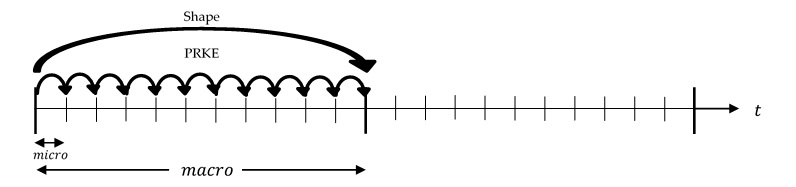
\includegraphics[width=\linewidth]{figures/IQS_visualization.jpg}
%\caption{IQS method visualization}
%\label{fig:iqsviz}
%\end{figure}
%
Note that the PRKE parameters are evaluated at each macro step and interpolated for the PRKE evaluation. In order to preserve 
the error convergence rate of high order temporal discretization schemes for shape, higher order interpolation of the parameters is required. \DIFdelbegin \DIFdel{A }\DIFdelend \DIFaddbegin \DIFadd{In this paper, a }\DIFaddend third-order implicit Runge-Kutta \cite{sdirk33} discretization with time-step adaptation is used for all PRKE \DIFdelbegin \DIFdel{evaluations in this paper }\DIFdelend \DIFaddbegin \DIFadd{solves }\DIFaddend in 
order to ensure a negligibly small error in the amplitude solution.

%---------------------------------------------------------------------------------------%
\subsection{IQS Iterative Schemes}
\label{sect:iter}
%---------------------------------------------------------------------------------------%

As noted in the previous section, shape-PRKE equations form a nonlinear system and must be solved in a iterative manner.  Over each macro time step,  one can 
use the latest end-time shape iterate to compute/interpolate the PRKE coefficients over the micro time step intervals. 
Sissaoui et al. from \cite{Sissaoui_1995}, Koclas et al. from \cite{Koclas_1996}, Devooght et al. from \cite{Devooght_1984}, and Monier from \cite{Monier_diss} all use 
iterative techniques for their IQS implementations.  They all undergo a similar process:
\begin{adjustwidth*}{0cm}{4mm}
 \begin{itemize} 
\item[\textit{Step 1:}] Compute the PRKE parameters at the end of the macro step using the last computed shape
\item[\textit{Step 2:}] \DIFdelbegin \DIFdel{Linearly interpolate }\DIFdelend \DIFaddbegin \DIFadd{Interpolate }\DIFaddend the computed PRKE parameters over the macro step
\item[\textit{Step 3:}] Solve the PRKE on micro steps over the entire macro step
\item[\textit{Step 4:}] Solve the shape equation on the macro step using the computed values of $p$ and $dp/dt$.
\item[\textit{Step 5:}] Check if the shape solution has converged:
	 \begin{itemize} 
	\item \textit{No:} Repeat the same macro time step
	\item \textit{Yes:} Move on to the next macro time step
	 \end{itemize} 
 \end{itemize} 
\end{adjustwidth*}

The major difference between the methods of these authors is the convergence criteria used.  Sissaoui and Koclas \cite{Sissaoui_1995, Koclas_1996} 
use fixed point iteration where the criteria is the simply the normalized difference between the last two computed shapes.  Monier in \cite{Monier_diss} 
also employs fixed point iterations with the same criteria, except that the solution is rescaled by $K_n/K_{n+1}$ after each iteration. Dulla in 
\cite{Dulla2008} does the same fixed-point iteration, but the shape is scaled by $K_0/K_{n+1}$ at the end of each macro time step. Renormalizing 
the shape is essential for preserving the uniqueness condition ($K_{n+1} = K_0$); this condition is not inherently conserved, even when the 
solution has converged from shape iterations.
\DIFaddbegin \DIFadd{It should be noted that Step 2 of the process generally involves a linear interpolation; however, for greater than second order shape discretizations, a higher-order interpolation was found to be necessary. 
}\DIFaddend 

These techniques are by no means an exhaustive list of the possible iteration techniques for IQS. Dulla et al. in \cite{Dulla2008} provide an 
in-depth analysis of the fixed-point iteration technique most similar to Sissaoui and Koclas, involving convergence rates and solution results.  
However, no comprehensive analysis of iteration techniques exists. The following describes 
each iteration convergence criterion investigated in this paper:

 \begin{itemize} 
\item $L^\infty$ norm of shape \cite{Monier_diss}: 
\[
\frac{\text{max}\left|\varphi_{n+1}^{(k+1)} - \varphi_{n+1}^{(k)}\right|}{\text{max}\left|\varphi_{n+1}^{(k+1)}\right|} < \epsilon_{\varphi}
\]
\item $L^2$ norm of shape: 
\[
\frac{\norm{\varphi_{n+1}^{(k+1)} - \varphi_{n+1}^{(k)}}}{\norm{\varphi_{n+1}^{(k+1)}}} < \epsilon_{\varphi}
\]
\item Reactivity convergence \cite{Monier_diss}: 
\[
\DIFaddbegin \left|\DIFaddend \left(\rho/\Lambda\right)^{(k+1)}_{n+1} - \left(\rho/\Lambda\right)^{(k)}_{n+1}\DIFaddbegin \right| \DIFaddend < \epsilon_{\rho}
\]
\item Amplitude convergence \cite{Monier_diss}: 
\[
\DIFaddbegin \left|\DIFaddend p_{n+1}^{(k+1)} - p_{n+1}^{(k)}\DIFaddbegin \right| \DIFaddend < \epsilon_p
\]
%\comm{why is this not a relative error criterion like the others? what's the rationale?}
%\answer{zmp}{I copied all of the above from \cite{Monier_diss}, not sure the rationale though}
\item Uniqueness consistency \cite{Monier_diss}: 
\[
\DIFaddbegin \left|\DIFaddend \frac{K_{n+1}^{(k+1)} - K_0}{K_0}\DIFaddbegin \right| \DIFaddend < \epsilon_K
\]
where $k$ denotes the nonlinear iteration index within a given macro time step interval.
 \end{itemize} 

In order to ensure that uniqueness criteria is preserved, some authors \cite{Monier_diss,Dulla2008} explicitly scale the shape solution, 
either at each nonlinear iteration or upon exiting the nonlinear loop on the macro time time step. This re-scaling is simply
\be 
\varphi^{g}_n \leftarrow \varphi^{g,(\text{last})}_n \frac{K_0}{K^{(\text{last})}_{n}} \,.
\label{eq:shape_scale}
\ee
%\comm{so, how does this jive with situations when the criterion on $K$ is employed?}
%\answer{zmp}{if the criteria is satisfied, it doesn't rescale; if it isn't, the solution is rescaled and another iteration is performed, the resulting solution isn't guaranteed to satisfy the criteria}

%---------------------------------------------------------------------------------------%
\subsection{IQS Predictor-Corrector Scheme}
%---------------------------------------------------------------------------------------%

The Predictor-Corrector version of the IQS method (\iqspc) is a linearized version of IQS, where no nonlinear iterations are required. The method relies on the shape and amplitude factorization of the flux and uniqueness condition. The PRKE derivation is identical to that of the standard (nonlinear) version of the IQS scheme, in the sense that shape solutions at the beginning and end times of the macro time interval are used (with interpolation in between). However, the manner in which the shape function is obtained is different.  In the \iqspc version, the flux equations (not the shape equations) are first solved (represented by \eqts{eq:flux}{eq:precursor}) in order to obtain a {\it predicted} flux solution at the end of the macro time step. This {\it predicted} flux is then converted to a shape by normalizing it as follows:

\be
\varphi^g_{n+1} = \underbrace{\phi^g_{n+1}}_{\text{predicted}} \frac{K_0}{\mathcal{K}_{n+1}} \,,
\label{eq:rescale}
\ee
where the flux scaling factor is given by
\be
\mathcal{K}_{n+1} =\sum_{g=1}^G\left(\phi^{*g},\frac{1}{v^g}\phi^g_{n+1}\right) \,,
\ee
and $K_0$ is the shape normalization constant (see \eqt{eq:normalization}).

The PRKE parameters are then computed with this shape using \eqtss{eq:rmb}{eq:l} and interpolated over the macro step, then the PRKE ODE system is solved on the micro time scale.  With the newly computed amplitude, the shape is rescaled into a flux and the final {\it corrected} flux is given by:

\be
\underbrace{\phi^g_{n+1}}_{\text{corrected}} = p_{n+1} \times \varphi^g_{n+1} \,.
\ee

The advantage to the predictor-corrector method is that no nonlinear iterations are necessary in this method; it is simpler to implement and can be faster than the standard IQS.  Ikeda et al. in \cite{Ikeda_2001} and Goluoglu et al. in \cite{Goluoglu_2001} 
both use \iqspc for complex, three-dimensional problems.  Their results prove \iqspc to be effective.  Dulla et al. in \cite{Dulla2008} also describes an in-depth comparison of \iqspc with traditional IQS\DIFdelbegin \DIFdel{, which originally brought the method to light. }\DIFdelend \DIFaddbegin \DIFadd{. %DIF > , which originally brought the method to light.
}\DIFaddend 

%---------------------------------------------------------------------------------------%
\subsection{Temperature Feedback Treatment}
%---------------------------------------------------------------------------------------%

Here, we consider multiphysics reactor physics simulations.  Fuel temperature feedback mechanisms are included using an adiabatic heat conservation model\DIFaddbegin \DIFadd{. For the purposes of this derivation, the adiabatic model, }\DIFaddend given in \eqt{eq:temp}\DIFaddbegin \DIFadd{, has linear heat capacity. However, a nonlinear heat capacity can easily be implemented with a iterative procedure}\DIFaddend . 
\be
\rho \DIFdelbegin \DIFdel{c}\DIFdelend \DIFaddbegin \DIFadd{C}\DIFaddend _p \frac{\partial T(\vec{r},t)}{\partial t} = \kappa_f \sum^G_{g=1}\Sigma_f^g \phi^g(\vec{r},t)
\label{eq:temp}
\ee
The thermal-range cross section's dependence on temperature is described by \eqt{eq:dopp}.
\be
\Sigma_a^{thermal}(\vec{r},t) = \Sigma_a^{thermal}(\vec{r},0)\left[1+\gamma\left(\sqrt{T}-\sqrt{T_0}\right)\right]
\label{eq:dopp}
\ee

A standard time-implicit solver for the heat equation would simply employ the flux values at the extremities of a time step interval.  However, in an IQS neutronic solve, much more information about space/time distribution of the flux is known: the shape distributions are typically known at the beginning and end of a macro time step interval but the amplitude is known on the micro-step time scale, providing a richer space/time information for the neutron flux over the macro-step interval. Thus, it is possible to solve for temperature in \eqt{eq:temp} using a semi-analytical approach, shown in \eqt{eq:temp_an}.
\be
T_{n+1} = T_n + \DIFdelbegin \DIFdel{\frac{\kappa_f}{\rho c_p} }\DIFdelend \DIFaddbegin \DIFadd{\frac{\kappa_f}{\rho C_p} }\DIFaddend \left(a_2 \varphi_{n+1} + a_1 \varphi_{n}\right)
\label{eq:temp_an}
\ee
where $n$ corresponds to the beginning of the temperature step.  $a_1$ and $a_2$ are integration coefficients 
given by \eqt{eq:a1} and \eqt{eq:a2}.  The shape function was assumed to vary linearly in time:
\be
\varphi(\vec{r},t) = \frac{t_{n+1}-t}{\Delta t}\varphi_{n}(\vec{r}) + \frac{t-t_n}{\Delta t}\varphi_{n+1}(\vec{r})  \,,
\ee
which leads to the coefficients' definitions:
\begin{subequations}
\be
a_1 = \int_{t_n}^{t_{n+1}}\left(\frac{t_{n+1}-t'}{\Delta t}\right)p(t')dt'
\label{eq:a1}
\ee
\be
a_2 = \int_{t_n}^{t_{n+1}}\left(\frac{t'-t_n}{\Delta t}\right)p(t')dt'
\label{eq:a2}
\ee
\end{subequations}
Because the amplitude $p$ is known on a fine time scale, the integrals \eqt{eq:a1} and \eqt{eq:a2}
are carried out along the micro steps, using a linear interpolant for the amplitude.

Temperature feedback affects both the shape equation and the reactivity coefficients of the PRKE; thus, 
it is an additional nonlinear component to the already coupled shape-amplitude equations. In foresight to 
the application of this component, we expect temperature to be more rapidly varying than the shape, but 
less so than the amplitude.  Therefore, the evaluation of temperature will have its own time scale, intermediary
between the amplitude's fine time scale and the shape's coarse time scale. 
\DIFaddbegin \DIFadd{This idea stems from the fact that in an adiabatic temperature model, the temperature's spatial variation follows the neutron flux shape, while the temperature amplitude follows the flux amplitude. Because of the heat capacity of the fuel, the temperature amplitude is often more slowly varying in time than neutron amplitude function itself, while still considerably faster varying than the flux shape. This conjecture is empirically defended in the results of Section 5.
}\DIFaddend Hence, a possible solution process for a problem with temperature feedback will have three time scales, as
portrayed in \fig{fig:time}.  The first time scale is the shape solve, the second is the temperature evaluation 
as well as the computation of PRKE parameters, and the third is the PRKE scale.  It is important to note that the 
number of time steps in each scale is arbitrary and the number chosen in \fig{fig:time} are only meant for 
illustrative purposes.

\begin{figure}[htpb!]
\centering
\resizebox{\linewidth}{!}{
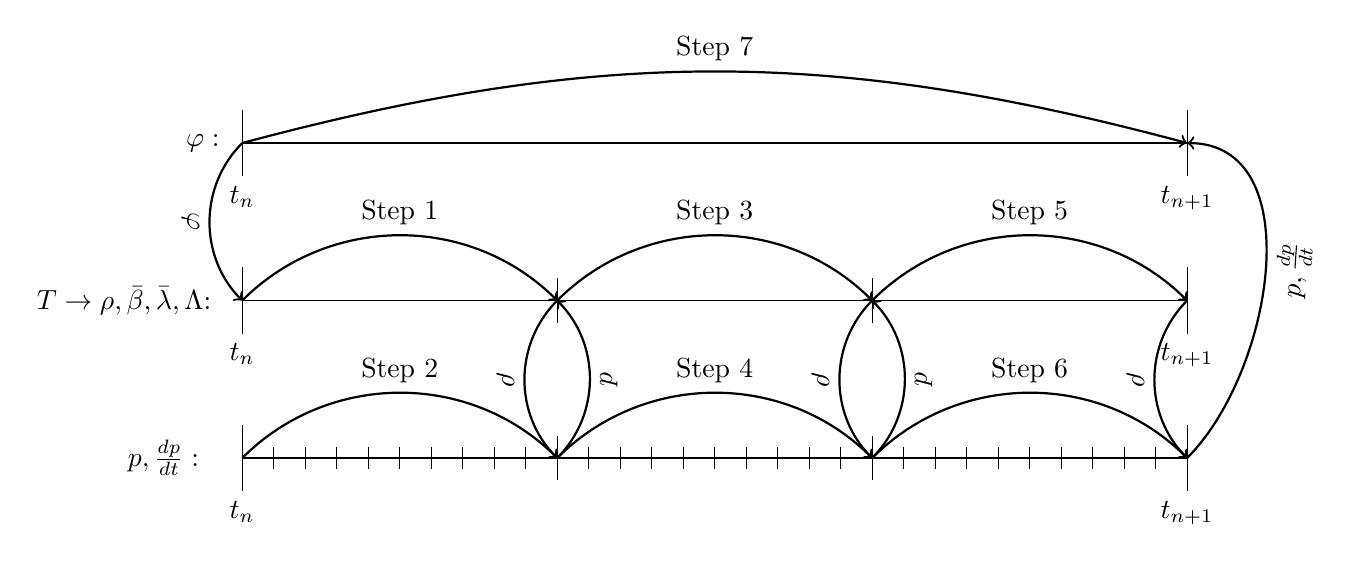
\begin{tikzpicture}[scale=2]
%Shape
\draw[] (0,2) -- (6,2) ;
\foreach \x in  {0,6}
\draw[shift={(\x,2)},color=black] (0pt,6pt) -- (0pt,-6pt);
\draw[shift={(0,2)},color=black] (0pt,0pt) -- (0pt,-6pt) node[below] {$t_n$};
\draw[shift={(6,2)},color=black] (0pt,0pt) -- (0pt,-6pt) node[below] {$t_{n+1}$};
\node(shape) at (-.25,2) {$\varphi:$};

%Temp/Params
\draw[] (0,1) -- (6,1) ;
\foreach \x in  {0,6}
\draw[shift={(\x,1)},color=black] (0pt,6pt) -- (0pt,-6pt);
\foreach \x in  {2,4}
\draw[shift={(\x,1)},color=black] (0pt,4pt) -- (0pt,-4pt);
\draw[shift={(0,1)},color=black] (0pt,0pt) -- (0pt,-6pt) node[below] {$t_n$};
\draw[shift={(6,1)},color=black] (0pt,0pt) -- (0pt,-6pt) node[below] {$t_{n+1}$};
\node(temp) at (-.75,1) {$T \rightarrow \rho, \bar{\beta}, \bar{\lambda}, \Lambda$:};

% PRKE
\draw[] (0,0) -- (6,0) ;
\foreach \x in  {0,6}
\draw[shift={(\x,0)},color=black] (0pt,6pt) -- (0pt,-6pt);
\foreach \x in  {0,2,4,6}
\draw[shift={(\x,0)},color=black] (0pt,4pt) -- (0pt,-4pt);
\foreach \x in  {0,0.2,0.4,0.6,0.8,1,1.2,1.4,1.6,1.8,2,2.2,2.4,2.6,2.8,3,3.2,3.4,3.6,3.8,4,4.2,4.4,4.6,4.8,5,5.2,5.4,5.6,5.8,6}
\draw[shift={(\x,0)},color=black] (0pt,2pt) -- (0pt,-2pt);
\draw[shift={(0,0)},color=black] (0pt,0pt) -- (0pt,-6pt) node[below] {$t_n$};
\draw[shift={(6,0)},color=black] (0pt,0pt) -- (0pt,-6pt) node[below] {$t_{n+1}$};
\node(prke) at (-.5,0) {$p, \frac{dp}{dt}:$};

\draw (0,0) edge[out=45,in=135,->,thick] node[above,sloped] {Step 2} (2,0);
\draw (2,0) edge[out=45,in=135,->,thick] node[above,sloped] {Step 4} (4,0);
\draw (4,0) edge[out=45,in=135,->,thick] node[above,sloped] {Step 6} (6,0);
\draw (0,1) edge[out=45,in=135,->,thick] node[above,sloped] {Step 1} (2,1);
\draw (2,1) edge[out=45,in=135,->,thick] node[above,sloped] {Step 3} (4,1);
\draw (4,1) edge[out=45,in=135,->,thick] node[above,sloped] {Step 5} (6,1);
\draw (0,2) edge[out=15,in=165,->,thick] node[above,sloped] {Step 7} (6,2);

\draw (0,2) edge[out=-135,in=135,->,thick] node[below,sloped] {$\varphi$} (0,1);
\draw (2,1) edge[out=-135,in=135,->,thick] node[below,sloped] {$\rho$} (2,0);
\draw (2,0) edge[out=45,in=-45,->,thick] node[below,sloped] {$p$} (2,1);
\draw (4,1) edge[out=-135,in=135,->,thick] node[below,sloped] {$\rho$} (4,0);
\draw (4,0) edge[out=45,in=-45,->,thick] node[below,sloped] {$p$} (4,1);
\draw (6,1) edge[out=-135,in=135,->,thick] node[below,sloped] {$\rho$} (6,0);
\draw (6,0) edge[out=45,in=0,->,thick] node[below,sloped] {$p, \frac{dp}{dt}$} (6,2);

\end{tikzpicture}
}
\caption{Time scales and process of IQS solve with temperature feedback}
\label{fig:time}
\end{figure}

Iteration processes are needed in between each time scale.  The amplitude and temperature need to be iterated on the middle 
time scale until convergence on each temperature step.  Then another iterative process needs to occur in the shape time scale on 
all three variables. \fig{fig:proc} shows the \DIFdelbegin \DIFdel{programming diagram implement }\DIFdelend \DIFaddbegin \DIFadd{solution workflow implemented }\DIFaddend to execute this process. 
\DIFdelbegin \DIFdel{The time increment of 
$\Delta t/3$ for the temperature solve is arbitrary and is meant only to match \fig{fig:time} where three temperature updates have been used as illustration.
}\DIFdelend \DIFaddbegin \DIFadd{$N_T$ is the number of temperature updates per macro step.
%DIF > The time increment of $\Delta t/3$ for the temperature solve is arbitrary and is meant only to match \fig{fig:time} where three temperature updates have been used as illustration.
}\DIFaddend 

\begin{figure}[!htpb]
\centering
\DIFdelbeginFL %DIFDELCMD < \resizebox{\linewidth}{!}{
%DIFDELCMD < \begin{tikzpicture}[every node/.style = {font=\normalsize}]
%DIFDELCMD < 

%DIFDELCMD < \node[greenblock](p1) at (0,0) {Save Old Solution};
%DIFDELCMD < \node[greenblock](p2) at (0,-2.5) {Save Current Solution};
%DIFDELCMD < \node[greenblock](p3) at (0,-5) {Interpolate Solution};
%DIFDELCMD < \node[blueblock2](p4) at (0,-7.5) {Solve Temperature};
%DIFDELCMD < \node[greenblock] (p5) at (0,-10) {Update PRKE Params};
%DIFDELCMD < \node[greenblock] (p6) at (0,-12.5) {Solve PRKE};
%DIFDELCMD < \node[reddiamond] (check1) at (0,-17.5) {Check for \\ convergence ($p$)};
%DIFDELCMD < \node[reddiamond] (check2) at (7,-12) {If $t=t_{n+1}$};
%DIFDELCMD < \node[greenblock] (p7) at (8,-6) {Shape Solve};
%DIFDELCMD < \node[reddiamond] (check3) at (8,-2.5) {Check for \\ convergence ($\varphi$)};
%DIFDELCMD < %\node [above =0.1mm of p1] {\large{IQS Solve:}};
%DIFDELCMD < %\node [above =0.1mm of p5] {\large{Multi-physics:}};
%DIFDELCMD < 

%DIFDELCMD < %\tikzback{p1}{p1}{p4}{p4}{bk1}
%DIFDELCMD < %\tikzback{p5}{p5}{p5}{p5}{bk2}
%DIFDELCMD < 

%DIFDELCMD < \draw[->,ultra thick](p1.south) -- node[right] {$t=t_{n+1}$}(p2.north);
%DIFDELCMD < \draw[->,ultra thick](p2.south) -- node[right] {$t=t_{n}+\Delta t/3$}(p3.north);
%DIFDELCMD < \draw[->,ultra thick](p3.south) -- (p4.north);
%DIFDELCMD < \draw [->,ultra thick] (p4.south)-- (p5.north);
%DIFDELCMD < \draw[->,ultra thick](p5.south) -- (p6.north);
%DIFDELCMD < \draw[->,ultra thick](p6.south) -- (check1.north);
%DIFDELCMD < \draw[->,ultra thick](check1.west) -- node[above,sloped] {\large{no}} (-5,-17.5) |-  (p4.west);
%DIFDELCMD < \draw[->,ultra thick](check1.east) -| node[right] {\large{yes}} (check2.south);
%DIFDELCMD < \draw[->,ultra thick](check2.west) -- node[above,sloped] {\large{no}\small \qq $t=t+\Delta t/3$} (4,-5) -- (p3.east);
%DIFDELCMD < \draw[->,ultra thick](check2.north) --  (8,-10) -- node[right] {\large{yes}} (p7.south);
%DIFDELCMD < \draw[->,ultra thick](p7.north) -- (check3.south);
%DIFDELCMD < \draw[->,ultra thick](check3.west) -- node[above] {no} (p2.east);
%DIFDELCMD < \draw[->,ultra thick](check3.north) -- node[right] {yes} (8,0) -- node[above] {$t_n=t_{n+1}$} (p1.east);
%DIFDELCMD < 

%DIFDELCMD < \end{tikzpicture}
%DIFDELCMD < }
%DIFDELCMD < %%%
\DIFdelendFL \DIFaddbeginFL \resizebox{\linewidth}{!}{
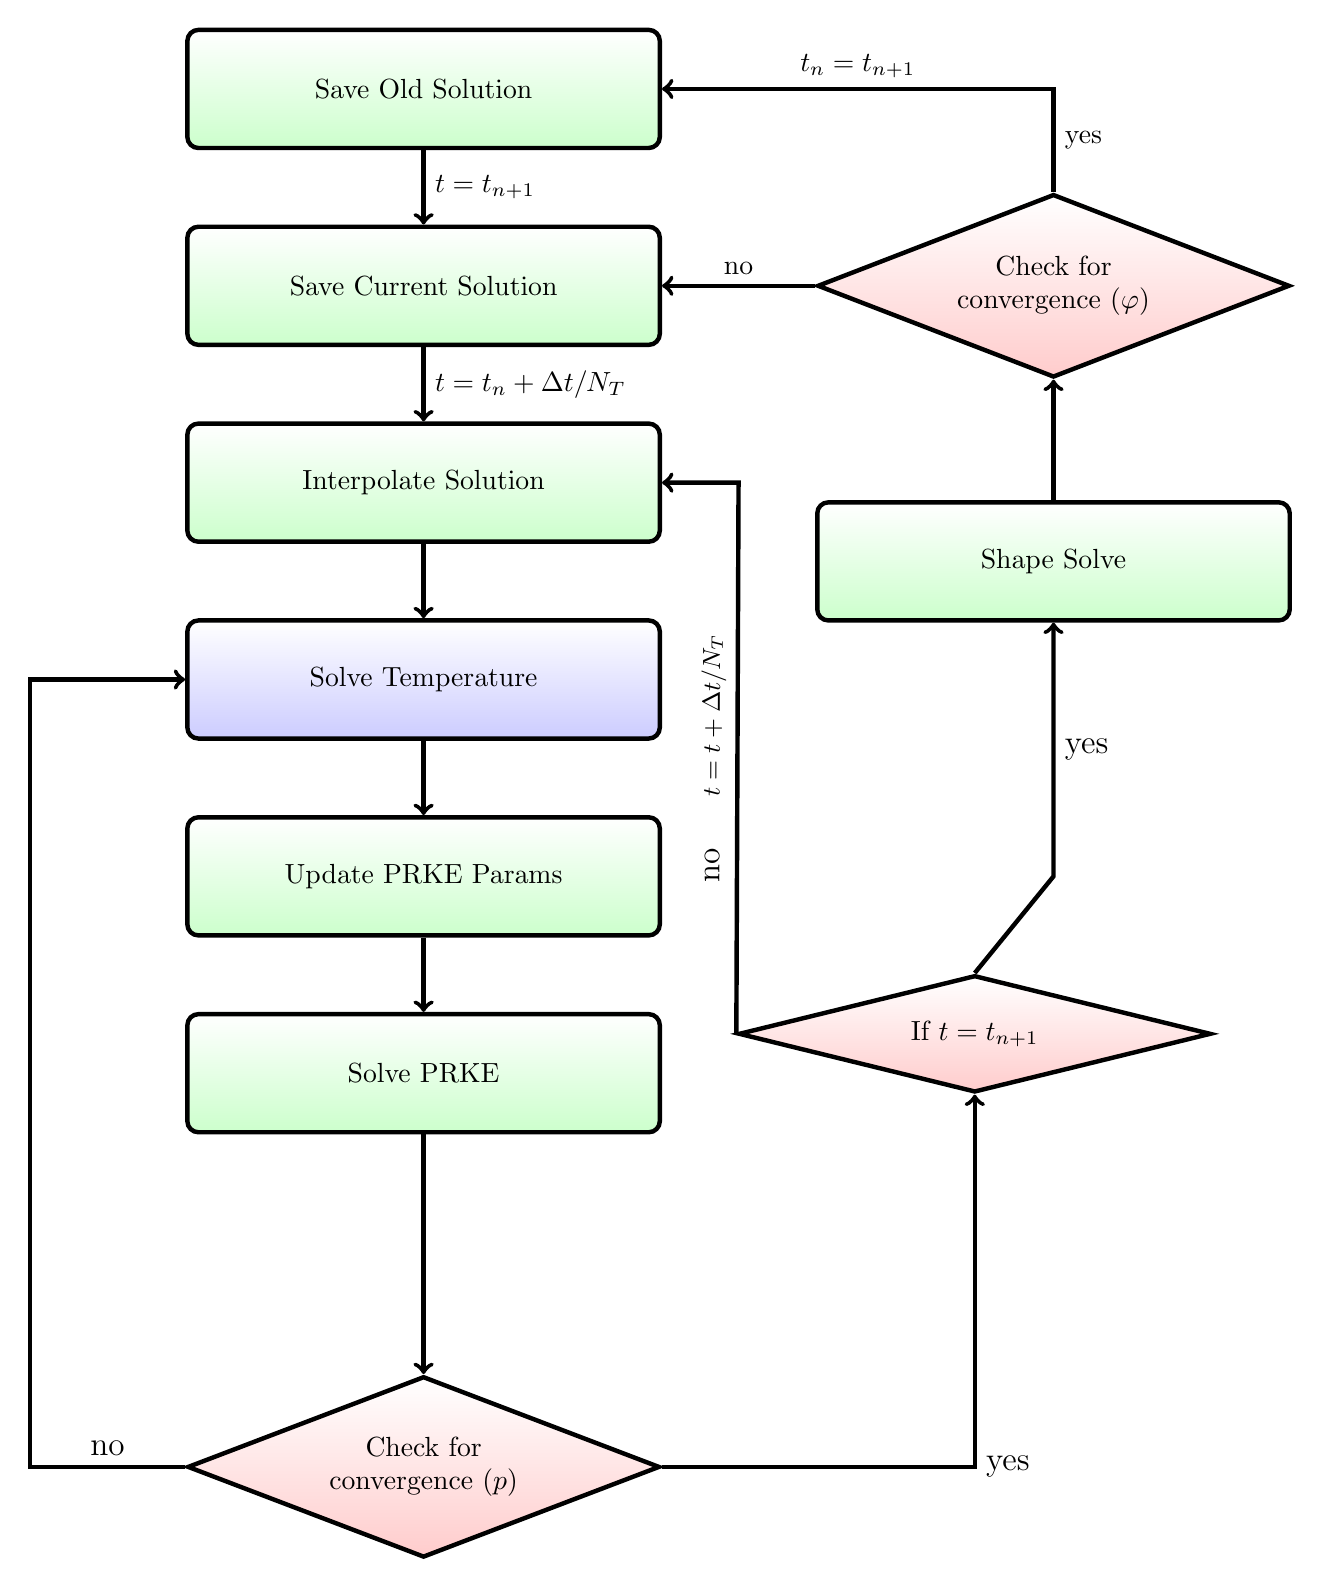
\begin{tikzpicture}[every node/.style = {font=\normalsize}]

\node[greenblock](p1) at (0,0) {Save Old Solution};
\node[greenblock](p2) at (0,-2.5) {Save Current Solution};
\node[greenblock](p3) at (0,-5) {Interpolate Solution};
\node[blueblock2](p4) at (0,-7.5) {Solve Temperature};
\node[greenblock] (p5) at (0,-10) {Update PRKE Params};
\node[greenblock] (p6) at (0,-12.5) {Solve PRKE};
\node[reddiamond] (check1) at (0,-17.5) {Check for \\ convergence ($p$)};
\node[reddiamond] (check2) at (7,-12) {If $t=t_{n+1}$};
\node[greenblock] (p7) at (8,-6) {Shape Solve};
\node[reddiamond] (check3) at (8,-2.5) {Check for \\ convergence ($\varphi$)};
%\node [above =0.1mm of p1] {\large{IQS Solve:}};
%\node [above =0.1mm of p5] {\large{Multi-physics:}};

%\tikzback{p1}{p1}{p4}{p4}{bk1}
%\tikzback{p5}{p5}{p5}{p5}{bk2}

\draw[->,ultra thick](p1.south) -- node[right] {$t=t_{n+1}$}(p2.north);
\draw[->,ultra thick](p2.south) -- node[right] {$t=t_{n}+\Delta t/N_{T}$}(p3.north);
\draw[->,ultra thick](p3.south) -- (p4.north);
\draw [->,ultra thick] (p4.south)-- (p5.north);
\draw[->,ultra thick](p5.south) -- (p6.north);
\draw[->,ultra thick](p6.south) -- (check1.north);
\draw[->,ultra thick](check1.west) -- node[above,sloped] {\large{no}} (-5,-17.5) |-  (p4.west);
\draw[->,ultra thick](check1.east) -| node[right] {\large{yes}} (check2.south);
\draw[->,ultra thick](check2.west) -- node[above,sloped] {\large{no}\small \qq $t=t+\Delta t/N_{T}$} (4,-5) -- (p3.east);
\draw[->,ultra thick](check2.north) --  (8,-10) -- node[right] {\large{yes}} (p7.south);
\draw[->,ultra thick](p7.north) -- (check3.south);
\draw[->,ultra thick](check3.west) -- node[above] {no} (p2.east);
\draw[->,ultra thick](check3.north) -- node[right] {yes} (8,0) -- node[above] {$t_n=t_{n+1}$} (p1.east);

\end{tikzpicture}
}
\DIFaddendFL \caption{Visualization of fixed-point iteration and temperature update process for IQS}
\label{fig:proc}
\end{figure}

%---------------------------------------------------------------------------------------%
\subsection{Delayed Neutron Precursor Treatment}
%---------------------------------------------------------------------------------------%

%This section presents the time-integration method used to solve coupled flux/shape and precursor equations, represented by Equations~\eqref{eq:flux}/\eqref{eq:shape}~and~\eqref{eq:precursor}/\eqref{eq:prec}. First, we note that we could keep this system of two time-dependent equations and solve it as a coupled system. However, this is unnecessary and a memory expensive endeavor because the precursor equation is only an ODE and not a PDE. Instead, one may discretize in time the shape equation, which typically requires the knowledge of the precursor concentrations at the end of the time step. This precursor value is taken from the solution, numerical or analytical, of the precursors ODE.

The precursors' equations, \eqt{eq:prec}, form a system of \DIFdelbegin \DIFdel{ODES}\DIFdelend \DIFaddbegin \DIFadd{ODEs}\DIFaddend . % ordinary differential equations.
A theta-scheme is often employed to evaluate the precursor concentrations:

\be
C_{n+1} = \frac{1-(1-\theta) \lambda\Delta t}{1+\theta \lambda\Delta t}C_n + \frac{(1-\theta) \beta\Delta t}{1+\theta \lambda\Delta t}S_{f,n} p_n +  \frac{\theta \beta\Delta t}{1+\theta \lambda\Delta t}S_{f,n+1} p_{n+1}
\label{eq:dnp_theta}
\ee
where $S_f$ is the fission source computed using the shape solution ($S_{f,n}=(\nu\Sigma_f)_n\varphi_n$). With
$\theta=1$, this yields the implicit Euler method, while with $\theta=\tfrac 1 2$, we obtain the Crank-Nicolson technique. In doing so, however, no micro-scale temporal information for the amplitude is used.
One can also solve the precursors' equations analytically, yielding:
\be
C_{n+1} =  C_n e^{-\lambda (t_{n+1} - t_n) }  + \int_{t_n}^{t_{n+1}} \beta(t') S_f(t') p(t')e^{-\lambda (t_{n+1}-t')}dt'
\label{eq:prec_an}
\ee
The shape function (using in $S_f$) is not known continuously over the time step but one may use the beginning/end times values
to linearly interpolate the fission source over the macro time step,
\be
S_f(t) = \frac{t_{n+1}-t}{\Delta t}S_{f,n}  + \frac{t-t_n}{\Delta t}S_{f,n+1}  \quad t_n \le t \le t_{n+1} \,.
\ee
Furthermore, a \DIFdelbegin \DIFdel{very accurate }\DIFdelend \DIFaddbegin \DIFadd{highly refined }\DIFaddend representation of $p(t)$ over the macro step is available from the PRKE solve (micro time scale). 
Using this fine scale information \DIFdelbegin \DIFdel{, the analytical }\DIFdelend \DIFaddbegin \DIFadd{yields a more precise integration of amplitude than assuming an interpolation of the amplitude between macro step points.
Applying this integration procedure, the semi-analytical }\DIFaddend solve for the precursor values yields
\be
C_{n+1} = C_n e^{-\lambda \Delta t} + \left(\hat{a}_2 S_{f,n+1}+\hat{a}_1 S_{f,n}\right)\beta \,,
\label{eq:dnp_an}
\ee
with integration coefficients defined as:
\begin{subequations}
\be
\hat{a}_1= \int_{t_n}^{t_{n+1}}\frac{t_{n+1}-t'}{\Delta t}p(t')e^{-\lambda(t_{n+1}-t')}dt' \,,
\ee
and
\be
\hat{a}_2 = \int_{t_n}^{t_{n+1}}\frac{t'-t_n}{\Delta t}p(t')e^{-\lambda(t_{n+1}-t')}dt'  \,.
\ee
\end{subequations}


%---------------------------------------------------------------------------------------%
\subsection{Step Doubling Time Adaptation}
%---------------------------------------------------------------------------------------%

Further enhancements to the performance of the IQS methods can be gained by using time adaptation (or time step control) in order to increase or reduce the macro time step size for the shape evaluation, depending on error estimates. A step-doubling technique is chosen as the time adaptation technique \cite{NumC}. The step doubling technique involves estimating the local error for a certain time step by taking the difference between a solution with one full step ($\varphi^g_{\Delta t}$) and a solution with two half steps ($\varphi^g_{\Delta t/2}$). Note: $\varphi$ \DIFaddbegin \DIFadd{(shape) }\DIFaddend is changed to $\phi$ \DIFaddbegin \DIFadd{(flux) }\DIFaddend in the case of the \iqspc technique. The relative error is computed as follows:
\be
e_n = \frac{\norm{\sum_{g=1}^G\varphi^g_{\Delta t/2} - \sum_{g=1}^G\varphi^g_{\Delta t}}}{\text{max}\left(\norm{\sum_{g=1}^G\varphi^g_{\Delta t/2}},\norm{\sum_{g=1}^G\varphi^g_{\Delta t}}\right)} \,.
\label{eq:edt2}
\ee
If the error is smaller than the user-specified tolerance, $e_{tol}$, the time step is accepted. In addition, a new time step size is estimated as follows:
\be
\Delta t_{new} = s \Delta t \left(\frac{e_{tol}}{e_n}\right)^{\frac{1}{1+q}} \,,
\label{eq:dt2}
\ee
where $q$ is the convergence order of the time integration scheme being used and $s\simeq 0.8$ is a safety factor. If the error is larger than the user-specified tolerance, the time step is rejected and new (smaller) macro time step size is estimated using \eqt{eq:edt2} as well. This process can be visualized by \figs{fig:dt2_1}{fig:dt2_2}, where a step involves a full convergence of shape, amplitude, and any multiphysics on the respective time step.

To investigate IQS's performance with step-doubling time adaptation, the adaptation \DIFdelbegin \DIFdel{will be applied to direct temporal }\DIFdelend \DIFaddbegin \DIFadd{is applied to implicit }\DIFaddend discretization of the flux equation (no IQS), the standard IQS method, and the \iqspc version. Each of these methods will be applied to several diffusion problems; the number of time steps taken and the resulting error will be used to compare the methods.

\begin{figure}[htpb!]
\centering
\resizebox{\linewidth}{!}{
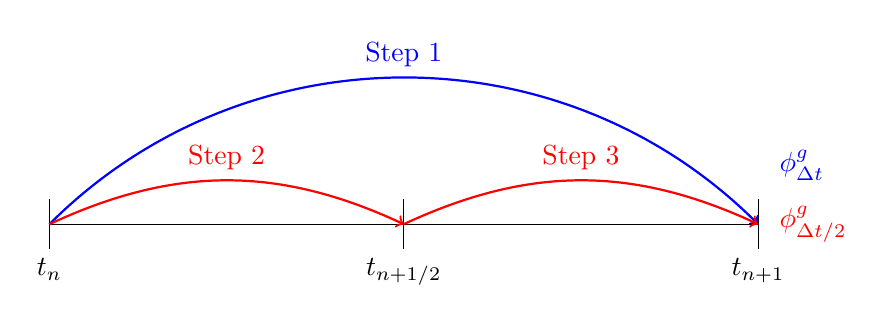
\begin{tikzpicture}[scale=1.5]
\draw[] (0,2) -- (6,2) ;
\foreach \x in  {0,3,6}
\draw[shift={(\x,2)},color=black] (0pt,6pt) -- (0pt,-6pt);
\draw[shift={(0,2)},color=black] (0pt,0pt) -- (0pt,-6pt) node[below] {$t_n$};
\draw[shift={(3,2)},color=black] (0pt,0pt) -- (0pt,-6pt) node[below] {$t_{n+1/2}$};
\draw[shift={(6,2)},color=black] (0pt,0pt) -- (0pt,-6pt) node[below] {$t_{n+1}$};
\draw (0,2) edge[out=45,in=135,->,thick,blue] node[above,sloped] {\tcb{Step 1}} (6,2);
\draw (0,2) edge[out=25,in=155,->,thick,red] node[above,sloped] {\tcr{Step 2}} (3,2);
\draw (3,2) edge[out=25,in=155,->,thick,red] node[above,sloped] {\tcr{Step 3}} (6,2);
\node[anchor=west](shape) at (6.1,2.5) {$\tcb{\phi_{\Delta t}^g}$};
\node[anchor=west](shape) at (6.1,2) {$\tcr{\phi_{\Delta t/2}^g}$};

\end{tikzpicture}
}
\caption{Visualization of step doubling process on time-line}
\label{fig:dt2_1}
\end{figure}

\begin{figure}[!htpb]
\centering
\resizebox{\linewidth}{!}{
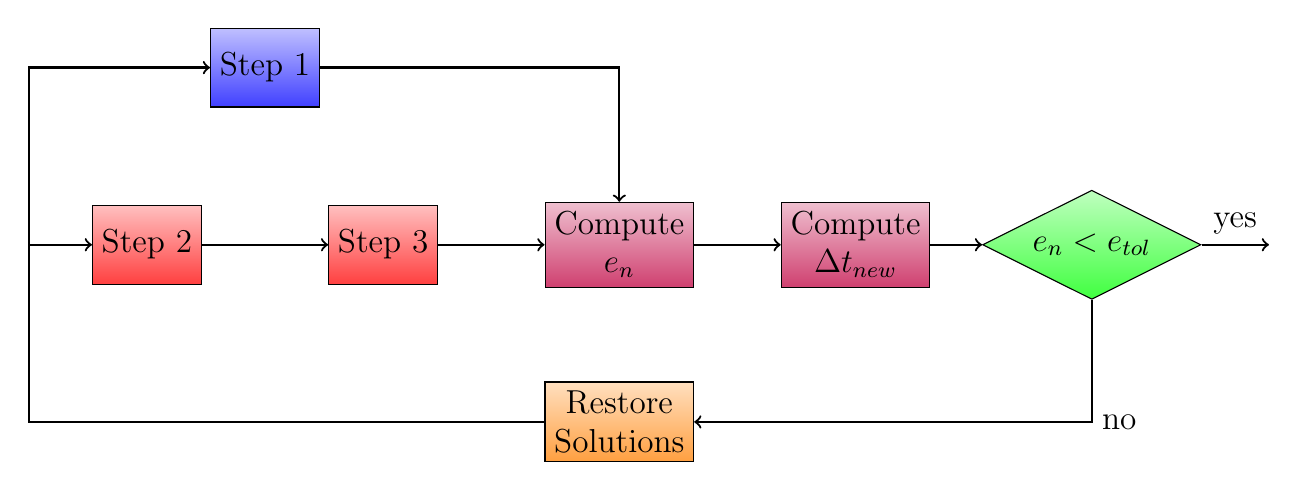
\begin{tikzpicture}[every node/.style = {font=\large},scale=0.75]

\node[blueblock](p1) at (-6,3) {Step 1} ;
\node[redblock](p2) at (-8,0) {Step 2} ;
\node[redblock](p3) at (-4,0) {Step 3} ;
\node[purpleblock](p4) at (0,0) {Compute \\ $e_n$};
\node[purpleblock](p5) at (4,0) {Compute  \\ $\Delta t_{new}$};
\node[greendiamond](p6) at (8,0) {$e_n < e_{tol}$};
\node[orangeblock](p7) at (0,-3) {Restore \\ Solutions};

\draw[->,thick](p1.east) -| (p4.north);
\draw[->,thick](p2.east) -- (p3.west);
\draw[->,thick](p3.east) -- (p4.west);
\draw[->,thick](p4.east) -- (p5.west);
\draw[->,thick](p5.east) -- (p6.west);
\draw[->,thick](p6.south) |- node[right] {no} (p7.east);
\draw[->,thick](p6.east) -- node[above] {yes} (11,0);
\draw[->,thick](p7.west) -| (-10,0) -- (p2.west);
\draw[->,thick](p7.west) -| (-10,0) |- (p1.west);

\end{tikzpicture}
}
\caption{Visualization of step doubling process with coding logic}
\label{fig:dt2_2}
\end{figure}

%%%%%%%%%%%%%%%%%%%%%%%%%%%%%%%%%%%%%%%%%%%%%%%%%%%%%%%%%%%%%%%%%%%%%%%%%%%%%%%%%%%%%%%%%
\section{Implementation in a multiphysics simulation environment}
%%%%%%%%%%%%%%%%%%%%%%%%%%%%%%%%%%%%%%%%%%%%%%%%%%%%%%%%%%%%%%%%%%%%%%%%%%%%%%%%%%%%%%%%%

Both the standard IQS and \iqspc methods have been implemented in the Multiphysics Object-Oriented Simulation Environment, MOOSE \cite{moose}, as part of its radiation transport solver, Rattlesnake \DIFdelbegin \DIFdel{\mbox{%DIFAUXCMD
\cite{wang2013}}%DIFAUXCMD
}\DIFdelend \DIFaddbegin \DIFadd{\mbox{%DIFAUXCMD
\cite{Rattlesnake_theory}}%DIFAUXCMD
}\DIFaddend . All multi-dimensional results presented here have been computed using the diffusion solver of Rattlesnake. The sequence of 
calculations in MOOSE (temporal loops, nonlinear loops, linear solves) with appropriate entry points at any level in the simulation allows for a relatively straightforward implementation of the IQS methodologies. MOOSE's nonlinear solvers (fixed-point iterations and Jacobian-free Newton-Krylov) are well suited to handle the nonlinear solve of the traditional IQS method during a macro time step. \iqspc's implementation in MOOSE is even simpler. We briefly describe the implementation next. 

\DIFaddbegin \DIFadd{A brief explanation of the MOOSE-specific objects for the IQS implementation can be seen below:
} \begin{itemize} 
\item \DIFadd{Kernel - Evaluation of the weak-form residual for a particular piece of physics.
}\item \DIFadd{Executioner - Establishes the type of simulation. The Transient type moves the simulation in time conducting spatial evaluations at each step.
}\item \DIFadd{Auxiliary variable and kernel - "Optional" variables that live on the same mesh as the solution and are computed algebraically using auxiliary kernels. 
}\item \DIFadd{Postprocessor - Computes scalar values over the entire spatial mesh, usually involves integrated quantities.
}\item \DIFadd{User-object - A generic type of postprocessor that allows connectivity of relevant quantities between different MOOSE objects.
} \end{itemize} 
\DIFadd{A more detailed and comprehensive description of MOOSE objects can be found in \mbox{%DIFAUXCMD
\cite{moose_training}}%DIFAUXCMD
.
}

\DIFaddend First, the IQS shape equation was represented by the gathering of appropriate finite element kernels. Most of the shape equation kernels are the same as the flux kernels already implemented in Rattlesnake for its standard diffusion (or transport) solution, and only two kernels had to be modified. \eqt{eq:kernels} shows which kernels needed to be written or amended (denoted by an \DIFdelbegin \DIFdel{$\star$}\DIFdelend \DIFaddbegin \DIFadd{$^\star$}\DIFaddend ) to solve the shape equation in MOOSE. The PRKE ODE was written as a sub-function in the Transient executioner, which advances the simulation in time and determines when to perform a shape (or flux for \iqspc) solve. This executioner has breakpoints that allows specified calls to the PRKE, PRKE parameter evaluation, and other multiphysics. The PRKE parameters are written as user-objects, looping over \DIFaddbegin \DIFadd{spatial mesh }\DIFaddend cells to evaluate them. Similarly, the semi-analytic treatment of fuel temperature and precursors are auxiliary kernels that do a node-by-node evaluation of the variable upon requests of the transient executioner. Additional information pertaining to these MOOSE objects can be found in \cite{PrinceTR2016}.

\begin{align}
\frac{1}{v^g}\frac{\partial\varphi^g}{\partial t}=&\underbrace{\frac{\chi_p^g}{\keff} \sum_{g'=1}^G (1-\beta) \nu^{g'} \Sigma_f^{g'} \varphi^{g'}}_{\textit{Prompt Production Kernel}} + \underbrace{\sum_{g'\neq g}^G\Sigma_s^{g'\to g} \varphi^{g'}}_{\textit{Scattering Kernel}} - \underbrace{\left( -\div D^g \grad \right)\varphi^g}_{\textit{Diffusion Kernel}} - \underbrace{\Sigma_r^g\varphi^g}_{\textit{Reaction Kernel}} \nonumber \\
& - \underbrace{\frac{1}{v^g} \boxed{\overbrace{\frac{1}{p}\frac{dp}{dt}}^{\textit{From PRKE}}}\varphi^g}_{\textit{IQS Reaction Kernel}^\star}+\underbrace{\frac{1}{p}\sum_{i=1}^I\chi_{d,i}^g\lambda_iC_i}_{\textit{Precursor Kernel}^\star}
\label{eq:kernels}
\end{align}


%First, it is important to note that MOOSE provides entry points in its calculation flow at various moments:
%\begin{itemize}
%\item during a time step, with a pre-step and post-step call;
%\item at each nonlinear iteration;
%\item at each linear iteration.
%\end{itemize}
%At each of these instants, an auxiliary calculations may be initiated (e.g., a convergence check, a full PRKE
%solve, a reactivity update, ...).  

%%%%%%%%%%%%%%%%%%%%%%%%%%%%%%%%%%%%%%%%%%%%%%%%%%%%%%%%%%%%%%%%%%%%%%%%%%%%%%%%%%%%%%%%%
\section{Neutronics-only Transient Results}
%%%%%%%%%%%%%%%%%%%%%%%%%%%%%%%%%%%%%%%%%%%%%%%%%%%%%%%%%%%%%%%%%%%%%%%%%%%%%%%%%%%%%%%%%

In this section, we analyze various convergence criteria proposed in the nonlinear solution technique for the IQS method. We also investigate the use of higher-temporal discretization for the shape equations. Both series of tests are carried out using neutronics-only problems.  The first test case uses a one-dimensional problem. The second test is from the ANL Benchmark Problem Book (BPB) \cite{ANL_BPB}. \DIFaddbegin \DIFadd{Note that any instance of $\Delta t$ in the following figures and commentary refers to the size of the macro time step.
}\DIFaddend 

%---------------------------------------------------------------------------------------%
\subsection{A One-Dimensional Problem}
%---------------------------------------------------------------------------------------%

This one-dimensional problem uses a 400-cm slab. This initial configuration is homogeneous and the transient is initiated by a perturbation in absorption cross section. \fig{fig:slab} shows problem layout and \tbl{tab:1Dmat} contains the material properties; one-group values are used for this problem. Regions 2, 3, and 4 have linear ramp perturbations at different moments in time, \tbl{tab:1Dslope} shows the values of the absorption cross-section in each region at the times of interest.  The values of $\Sigma_a$ between these times of interest vary linearly between the given values.

\begin{figure}[!htbp]
\begin{center}
\resizebox{\linewidth}{!}{
\begin{tabular}{| l | l | l | l | l | l | l | l | l | l | l | l | l | l | l | l | l | l | l | l |}
\hline \hline \hline
  &   &   &   &   &   &    &    &   &   &   &   &   &   &   &   &   &   &   &   \\
1 & 1 & 1 & 1 & 2 & 3 & 1 & 1 & 1 & 1 & 1 & 1 & 1 & 1 & 4 & 4 & 1 & 1 & 1 & 1 \\
  &   &   &   &   &   &    &    &   &   &   &   &   &   &   &   &   &   &   &   \\
\hline \hline \hline
\end{tabular}
}
\caption{1-D slab: Region identification number}
\label{fig:slab}
\end{center}
\end{figure}

\begin{table}[!htbp]
\begin{center}
\caption{1-D slab material properties and problem parameters}
\label{tab:1Dmat}
\resizebox{\linewidth}{!}{
\begin{tabular}{llllll}
\hline
$D (cm)$ & $\Sigma_a (cm^{-1})$ & $\nu \Sigma_f (cm^{-1})$ & $v (cm/s)$ & $\beta$ & $\lambda (s^{-1})$ \\
\hline
1.0 & 1.1 & 1.1 & 1,000 & 0.006 & 0.1 \\

\hline
\end{tabular}
}
\end{center}
\end{table}

\begin{table}[!htbp]
\begin{center}
\caption{1-D slab absorption \DIFdelbeginFL \DIFdelFL{cross-section }\DIFdelendFL \DIFaddbeginFL \DIFaddFL{cross sections }\DIFaddendFL at times of interest}
\label{tab:1Dslope}
\resizebox{\linewidth}{!}{
\begin{tabular}{llllllll}
\hline
Region & Material Property & 0.0 s & 0.1 s & 0.6 s & 1.0 s & 1.7 s \\
\hline
2 & $\Sigma_{a} (cm^{-1})$ & 1.1 & 1.1 & 1.095 & 1.095 & 1.095 \\
3 & $\Sigma_{a} (cm^{-1})$ & 1.1 & 1.1 & 1.09 & 1.09 & 1.1 \\
4 & $\Sigma_{a} (cm^{-1})$ & 1.1 & 1.1 & 1.105 & 1.105 & 1.105 \\
\hline
\end{tabular}
}
\end{center}
\end{table}

\fig{fig:1D} shows the reference flux solution at different instants as well as total power as a function of time.  The baseline reference solution was computed by solving the flux equations (not the IQS formulation) using time-step control with a tight relative error tolerance of $10^{-12}$. The problem being relatively large, the various zones are weakly coupled and the flux perturbation is not global. This baseline computation is used to compute the error of the other time discretization methods. \fig{fig:1D_shape} shows the shape profile at the same instants during the transient as in \fig{fig:1D_flux}; that solution was also obtained using time-step control with tight tolerance. Both flux solve and IQS solve yield the same answer, as expected.  
% Even though the magnitude of the shape varies less during the transient, its spatial distribution shows more variation than that 
% It is apparent that the shape is time-dependent, so it is expected that IQS has marginal accuracy gain for a given time step size.

\begin{figure}[!htbp]
\centering
\begin{subfigure}[b]{0.49\textwidth}
\centering
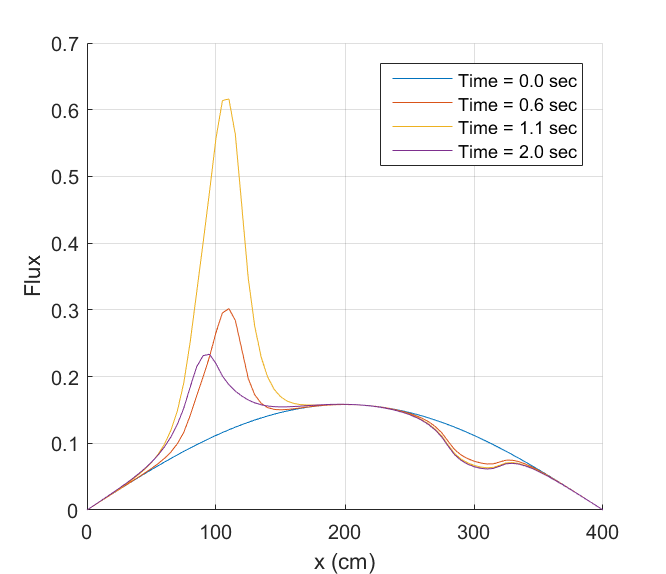
\includegraphics[width=0.99\textwidth]{figures/1D_flux.png}
\caption{Flux profile at various times}
\label{fig:1D_flux}
\end{subfigure}
\begin{subfigure}[b]{0.49\textwidth}
\centering
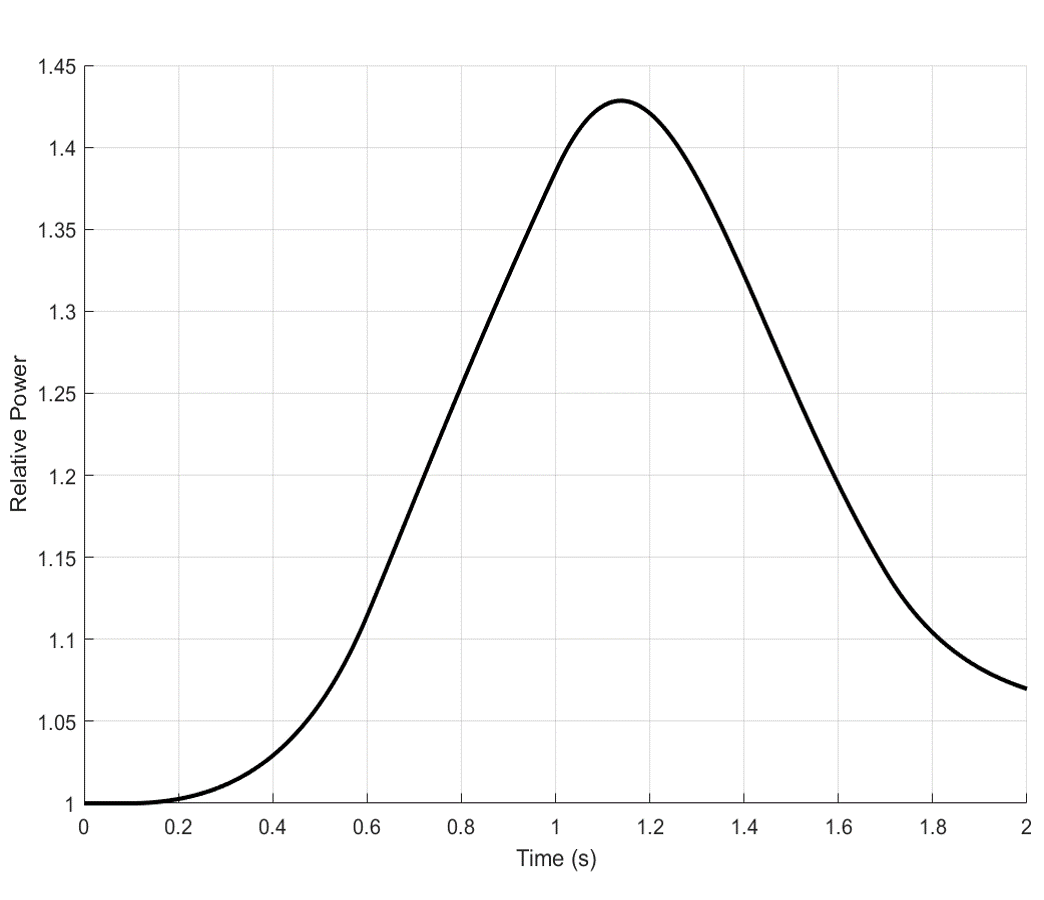
\includegraphics[width=0.99\textwidth]{figures/1D_power_base.png}
\caption{\DIFdelbeginFL \DIFdelFL{Power profile over transient}\DIFdelendFL \DIFaddbeginFL \DIFaddFL{Normalized total power as a function of time}\DIFaddendFL }
\label{fig:1D_tot_power}
\end{subfigure}
\caption{Baseline flux and power distribution}
\label{fig:1D}
\end{figure}

\begin{figure}[!htbp]
%\centering
%\begin{subfigure}[b]{0.49\textwidth}
\centering
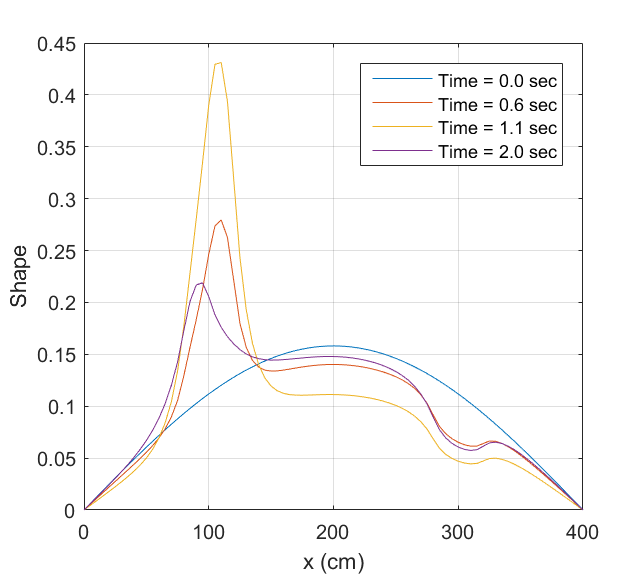
\includegraphics[width=0.49\textwidth]{figures/1D_shape2.png}
\caption{IQS Shape profile at various times}
\label{fig:1D_shape}
%\end{subfigure}
%\begin{subfigure}[b]{0.49\textwidth}
%\centering
%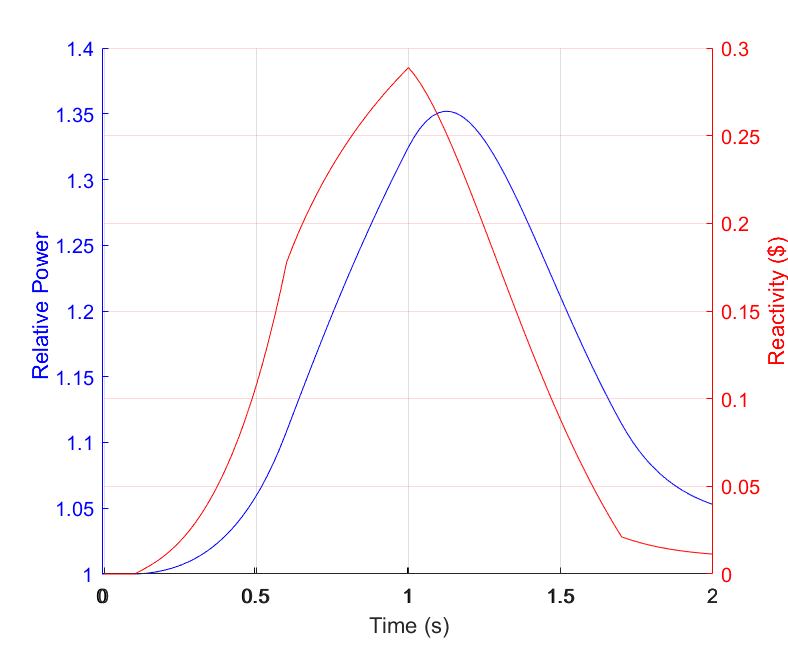
\includegraphics[width=0.99\textwidth]{figures/1D_iqs_power.png}
%\caption{Power and reactivity profile over transient}
%\end{subfigure}
%\caption{IQS flux and power distribution}
%\label{fig:1D_res}
\end{figure}
%\jcr{not sure that the Fig.7b is useful}

In the standard IQS technique, a nonlinear system of equations is to be solved for the shape and the amplitude solutions. \sct{sect:iter} lists various iteration stopping criteria typically employed with IQS. \fig{fig:iter} gives the number of fixed-point iterations required to reach tolerance of $10^{-11}$ as a function of time during the transient. A theta-scheme is employed for the precursors equations (\eqt{eq:dnp_theta}).
%The criteria listed in the legend correspond to the list as such:
%\begin{enumerate}
%\item $L^{\infty} \rightarrow$ 1.
%\item $L^{2} \rightarrow$ 2.
%\item Reactivity $\rightarrow$ 3.
%\item Amplitude $\rightarrow$ 4.
%\item $K$ criteria $\rightarrow$ 5.
%\item The last 3 criteria combined $\rightarrow$ 3.-5.
%\end{enumerate}
This figures shows that criteria based on the  $L^{\infty}$ norm of the shape, the $L^2$ norm of the shape, the reactivity change, and the amplitude have approximately the same convergence behavior, but the criteria based on the uniqueness constant $K$ never reaches the tight tolerance and runs up to the maximum number of iterations allowed (20 in this case). \fig{fig:iter_err} shows \DIFaddbegin \DIFadd{that }\DIFaddend the error in the \DIFaddbegin \DIFadd{uniqueness }\DIFaddend factor $K$ saturates to different levels, whether the shape is rescaled or not.
%Rescaling shape more frequently helps the error.  However, rescaling every iteration is somewhat artificial because it does not consider changes spatially. Regardless, an error of $~10^{-5}$ is quite large and it is expected that the magnitude is due to the explicit treatment of precursors (\eqt{eq:dnp_theta}). 
However, switching the precursors solve to be performed semi-analytically (\eqt{eq:dnp_an}) significantly improves the convergence in the uniqueness factor $K$, see \fig{fig:iter_err_an}. \DIFaddbegin \DIFadd{This result implies that uniqueness of the shape and amplitude can only be maintained with a consistent treatment of precursor term in the shape equation.
}\DIFaddend 

\begin{figure}[!htbp]
\centering
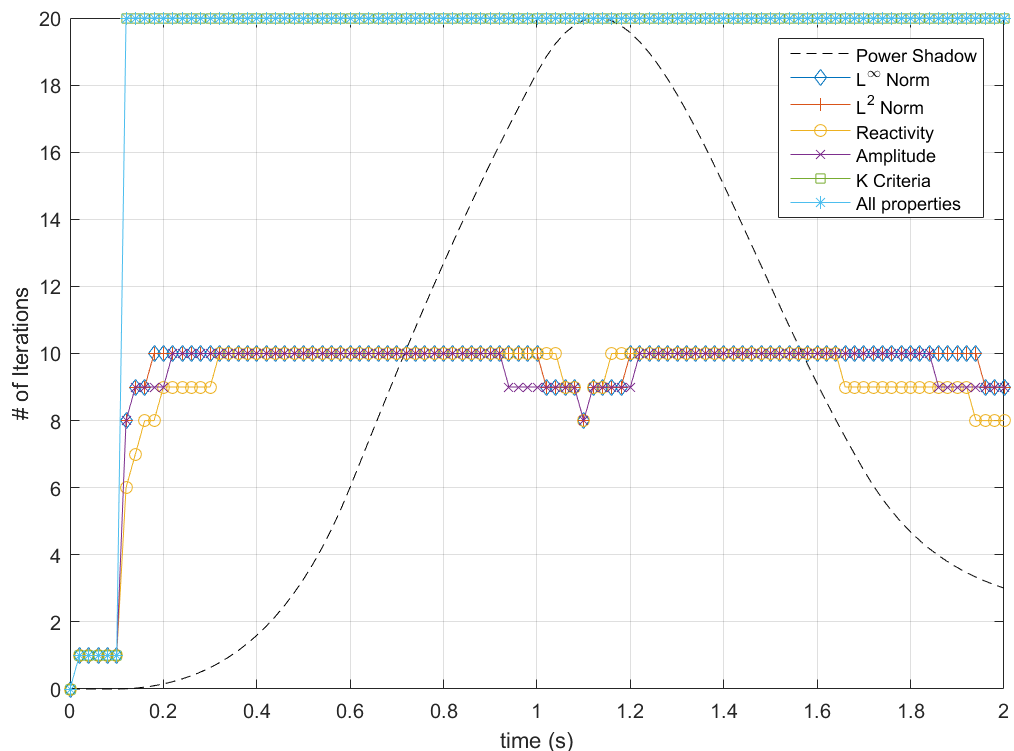
\includegraphics[width=0.49\textwidth]{figures/iter_renorm.png}
\caption{\# of iterations for various convergence criteria, tolerance$=10^{-11}$, max iterations$=20$}
\label{fig:iter}
\end{figure}

\begin{figure}[!htbp]
\centering
\begin{subfigure}[b]{0.49\textwidth}
\centering
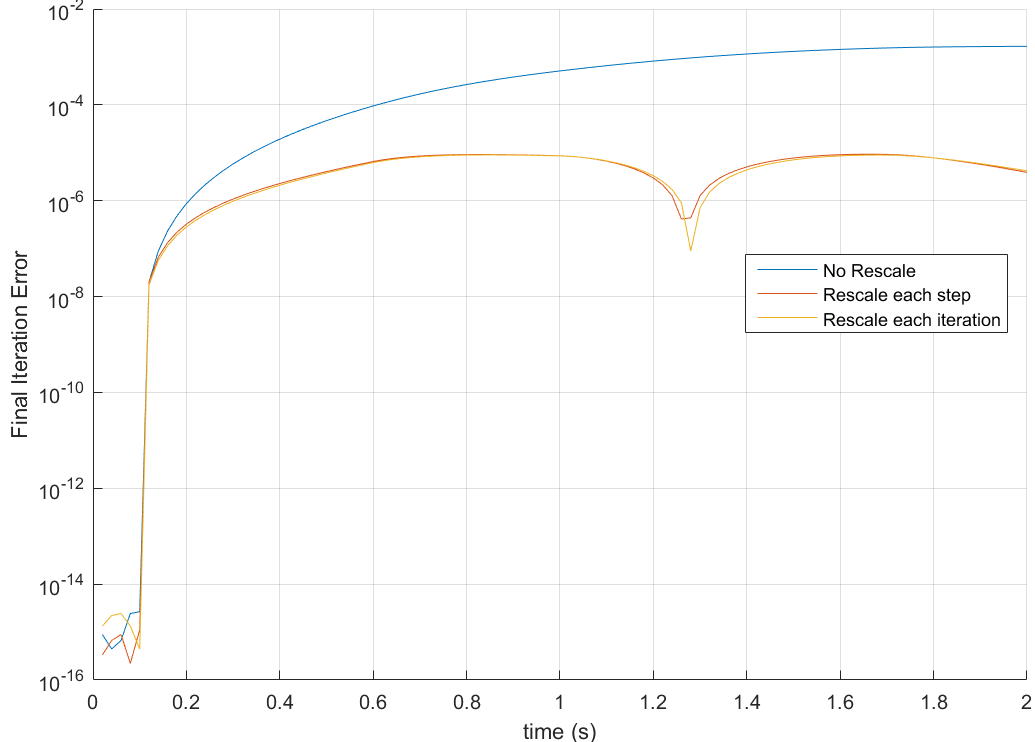
\includegraphics[width=0.99\textwidth]{figures/iter_error.png}
\caption{Precursors solved using a theta-scheme}
\label{fig:iter_err}
\end{subfigure}
\begin{subfigure}[b]{0.49\textwidth}
\centering
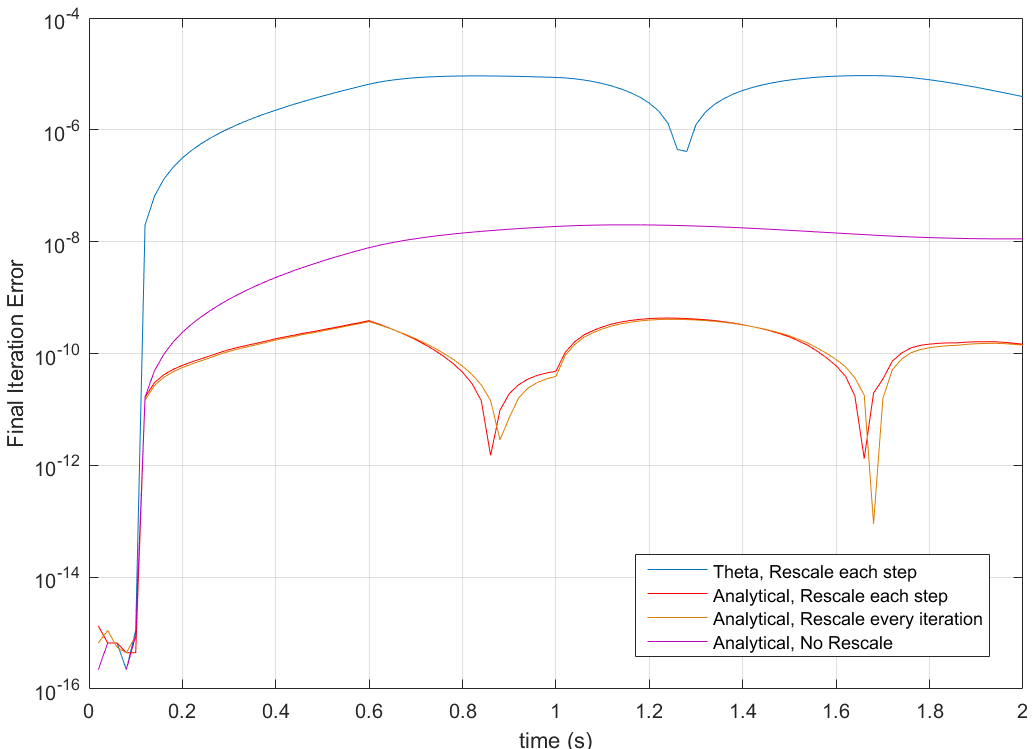
\includegraphics[width=0.99\textwidth]{figures/iter_error_an.png}
\caption{Analytical precursor solve}
\label{fig:iter_err_an}
\end{subfigure}
\caption{Final iteration error \DIFaddbeginFL \DIFaddFL{$\left(K_{n+1}^{(k+1)}/K_0 - 1\right)$ }\DIFaddendFL for $K$ factor convergence criterion}
\end{figure}

\clearpage
\newpage

%----------------------------------------------------------------------------------------
%\subsubsection{One-Dimensional Problem Time Step Convergence Analysis}

Next, we investigate the use of higher-order temporal methods to solve the shape equations (standard IQS and \iqspc methods). We compare these results with the same high-order discretization \DIFdelbegin \DIFdel{for }\DIFdelend \DIFaddbegin \DIFadd{of }\DIFaddend the flux equations. 
%Time step convergence analysis involves evaluating a problem with various refinements in step size and comparing the resulting errors with the time step size. Plotting error versus $\Delta t$ on a log-scale should produce a relatively strait line with a slope equal to the order of the time discretization method. In order to evaluate the performance and error convergence of IQS, the slab was simulated with varying time discretization methods and time step sizes.
\fig{fig:1D_conv} shows the convergence results for four different time-implicit discretization: backward difference formulae, from order 1, which is the same as the implicit Euler, to order 4. For a detailed description on BDF methods, see \cite{Gear:2007}. The plots show that IQS and \iqspc converge with the expected order (1 through 4) using BDF1 through BDF4. Recall that in the amplitude equations, the PRKE parameters are interpolated using the shape solutions. We used higher-order interpolants in time for the shape solution when a higher-order method was used (the convergence rates were degraded for higher-order BDF methods when the PRKE parameters were only linearly interpolated over the macro step). Lagrange and Hermite interpolants yielded the same results. In addition, we used semi-analytical integration of the precursors equations, along with the same higher-order interpolation of the shape values when a higher-order method was used. Without using the same order interpolants as the BDF formula, the error in the PRKE parameters and the precursors led to reduction in the observed convergence rate.

% The Third-order SDIRK method did not show third order convergence, but, through extensive testing, SDIRK shows non-convergent behavior for too stiff of problems.  

The convergence rates for the straightforward discretization of the flux equations are also shown in \fig{fig:1D_conv} and they followed the same expected convergence rates. These flux-solve results are indicated by the legend ``Implicit Dis.''. It is worthy to note that, for lower-order discretizations, the error in the flux equations is always significantly higher than that of the IQS results. However, as the order of the temporal scheme is increased, the gap between the discretization error in the flux equations and the IQS equations vanishes. In previous publications, the shape solves with the IQS method always employed a lower-order temporal discretization (often implicit Euler). Our results seem to indicate that a high-order discretization of the flux equations may reduce the usefulness of the IQS approach (at least for large domains with weakly coupled spatial regions). 
\DIFaddbegin \DIFadd{It should be noted that the baseline for these error computations was performed using an adaptive method for the flux equations with a tight tolerance. The proper convergence rates seen by the methods with coarser time steps show that this baseline is accurate enough for computing the error.
}\DIFaddend %This paper shows an analysis of the first publicized application of IQS with higher than second order discretization, which exposed unforeseen properties of IQS.  When using higher order techniques, the interpolation of PRKE parameters and shape for precursor integration become important to consider.  Every other application that was investigated linearly interpolates parameters for the PRKE evaluation.  Similarly, the shape used for the integration of the ODE for the precursors needs to have higher order interpolation to preserve high order error convergence.  This interpolation was done using Lagragian and Hermite methods, both leading to successful convergence.

\begin{figure*}[!htbp]
\centering
\begin{subfigure}[b]{0.49\textwidth}
\centering
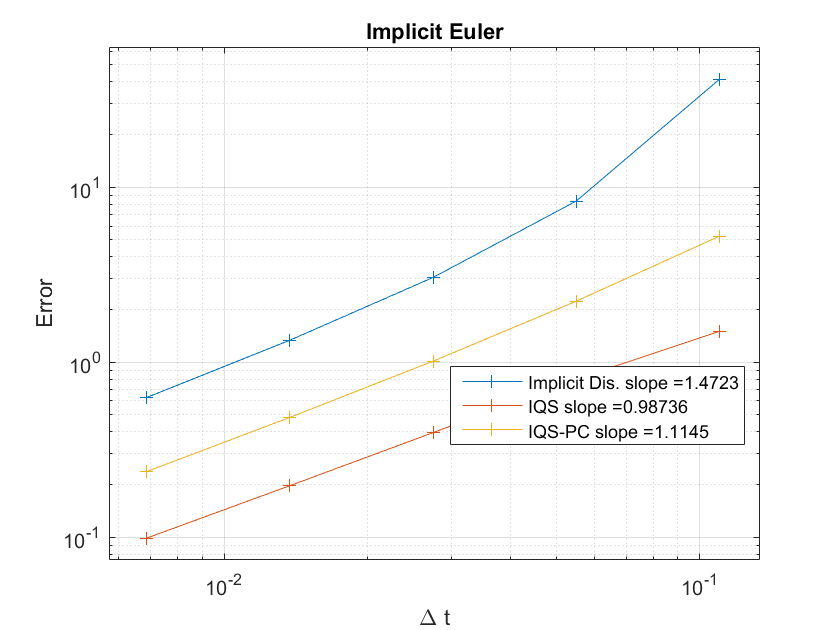
\includegraphics[width=\linewidth]{figures/1D_conv_IE.png}
\caption{Implicit Euler (BDF1)}
\end{subfigure}
\begin{subfigure}[b]{0.49\textwidth}
\centering
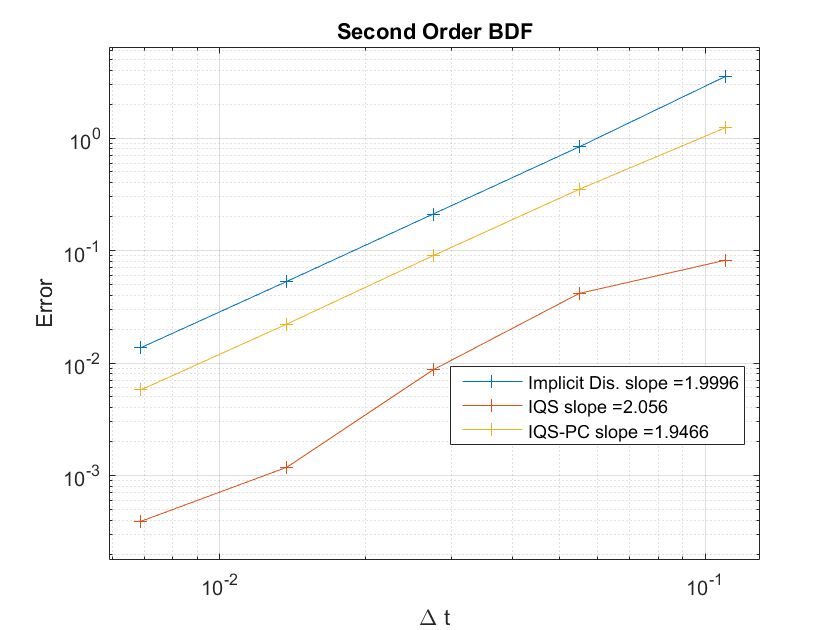
\includegraphics[width=\linewidth]{figures/1D_conv_BDF2.png}
\caption{BDF2}
\end{subfigure}
\begin{subfigure}[b]{0.49\textwidth}
\centering
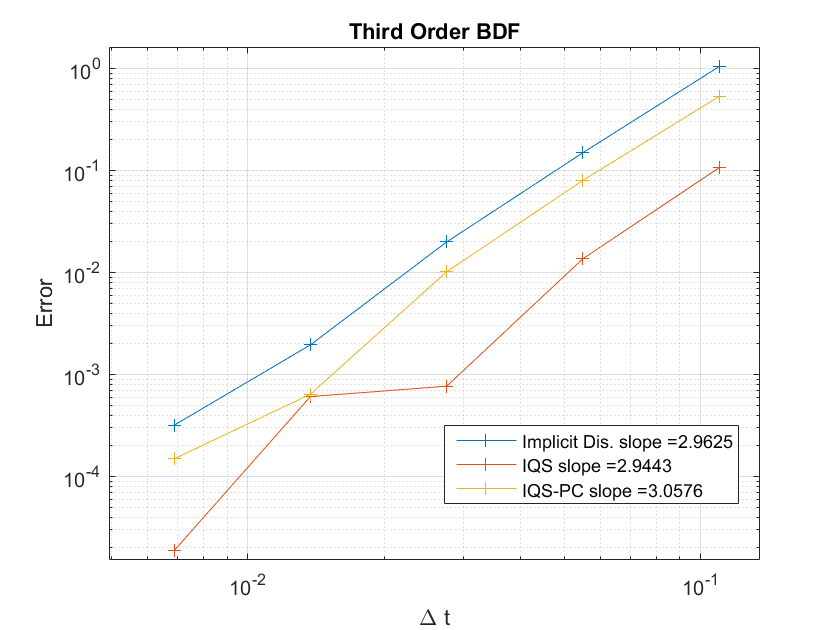
\includegraphics[width=\linewidth]{figures/1D_conv_BDF3.png}
\caption{BDF3}
\end{subfigure}
\begin{subfigure}[b]{0.49\textwidth}
\centering
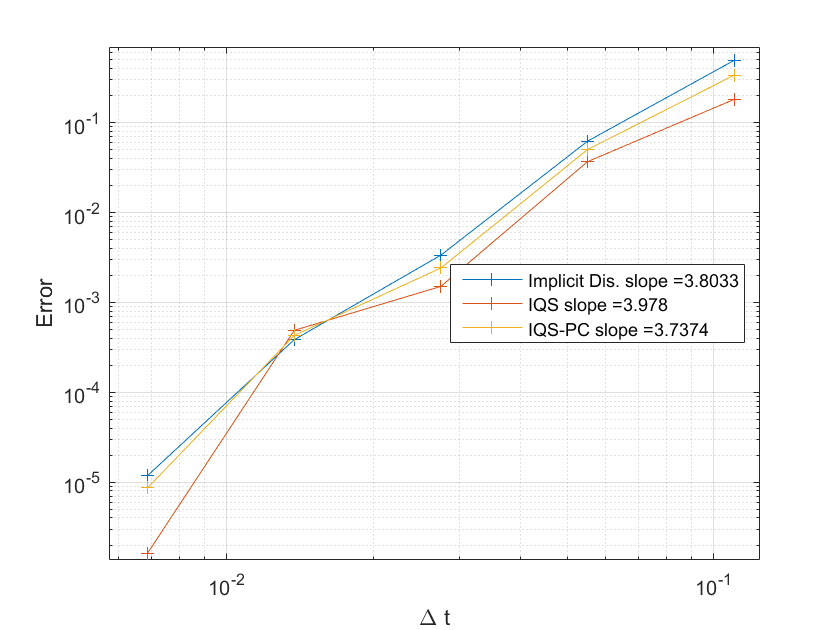
\includegraphics[width=\linewidth]{figures/1D_conv_BDF4.png}
\caption{BDF4}
\end{subfigure}
%\begin{subfigure}[b]{0.49\textwidth}
%\centering
%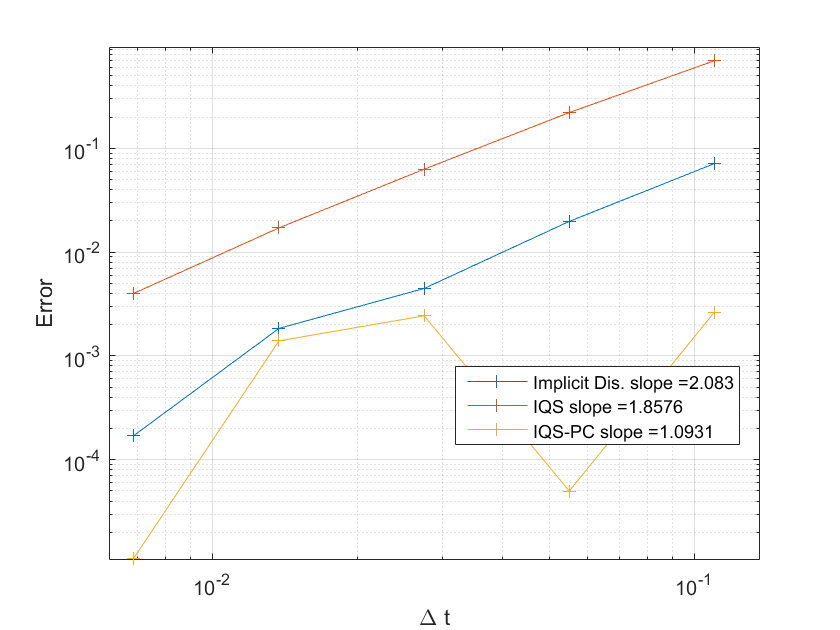
\includegraphics[width=\linewidth]{figures/1D_conv_SDIRK33.png}
%\caption{SDIRK33}
%\end{subfigure}
\caption{Error convergence plots of implicit discretization, IQS, and \iqspc with various time discretization schemes\DIFaddbeginFL \DIFaddFL{. Errors correspond to the relative difference in the peak power from the baseline solution.}\DIFaddendFL }
\label{fig:1D_conv}
\end{figure*}

%%----------------------------------------------------------------------------------------
%\subsubsection{One-Dimensional Mini-Core Problem}
%\jcr{i do not understand the purpose of the entire section. shouldn't the mini core be doen with bdf4 too, not just bdf1? and aren't the twigl results already such a demonstration so why not move on to twigl right away?}
%This problem is exactly the same as the previous one-dimensional problem, except the the core was reduced to 80 cm in length. The purpose of testing this problem is to determine if a more tightly coupled core will yield better performance for IQS. \fig{fig:1Dmini_flux} shows the resulting baseline flux and relative power profile of the one-dimensional mini-core problem. This plot shows that the perturbed regions affect the domain more evidently. \fig{fig:1Dmini_shape} shows the shape profile at various times during the transient. This plot shows that the shape is much less time-dependent than the previous large core. \fig{fig:1Dmini_conv} shows that IQS performs significantly better with this example than the large core.
%
%\begin{figure}[!htbp]
%\centering
%\begin{subfigure}[b]{\linewidth}
%\centering
%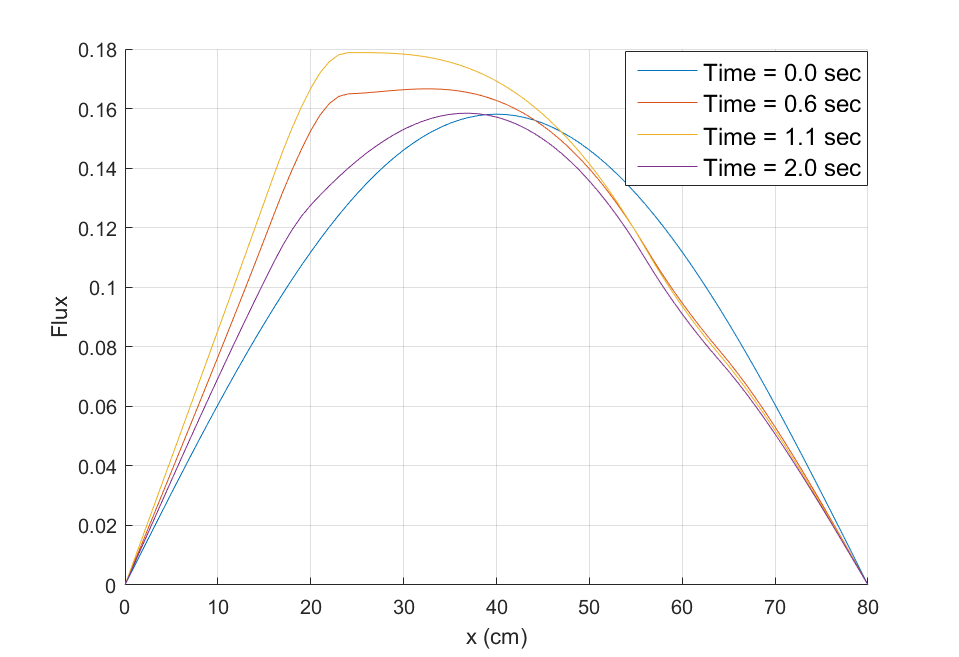
\includegraphics[height=1.5in]{figures/1Dmini_flux.png}
%\caption{Flux profile at various times}
%\end{subfigure}
%\begin{subfigure}[b]{\linewidth}
%\centering
%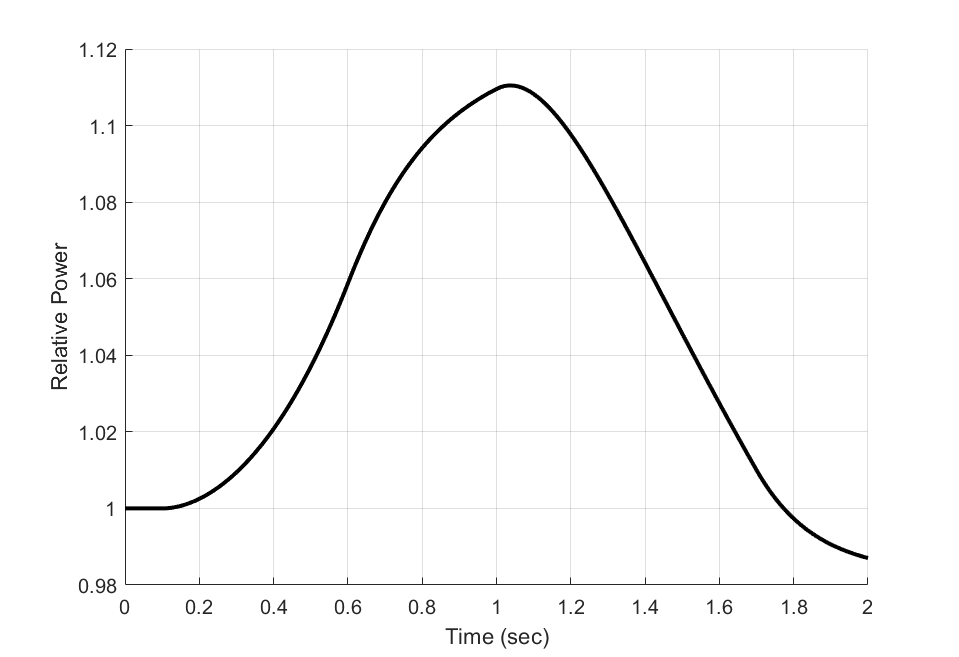
\includegraphics[height=1.5in]{figures/1Dmini_power_base.png}
%\caption{Power profile over transient}
%\end{subfigure}
%\caption{Mini-core baseline flux and power distribution}
%\label{fig:1Dmini_flux}
%\end{figure}
%
%\begin{figure}[!htbp]
%\centering
%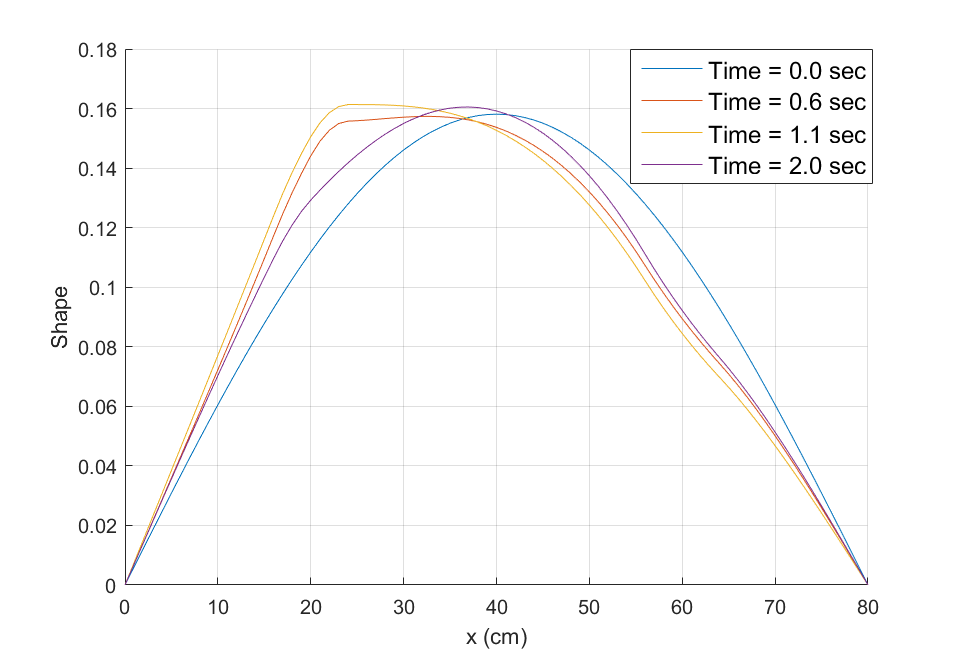
\includegraphics[height=1.5in]{figures/1Dmini_shape.png}
%\caption{Shape profile at various times for one-dimensional mini-core}
%\label{fig:1Dmini_shape}
%\end{figure}
%
%\begin{figure}[!htbp]
%\centering
%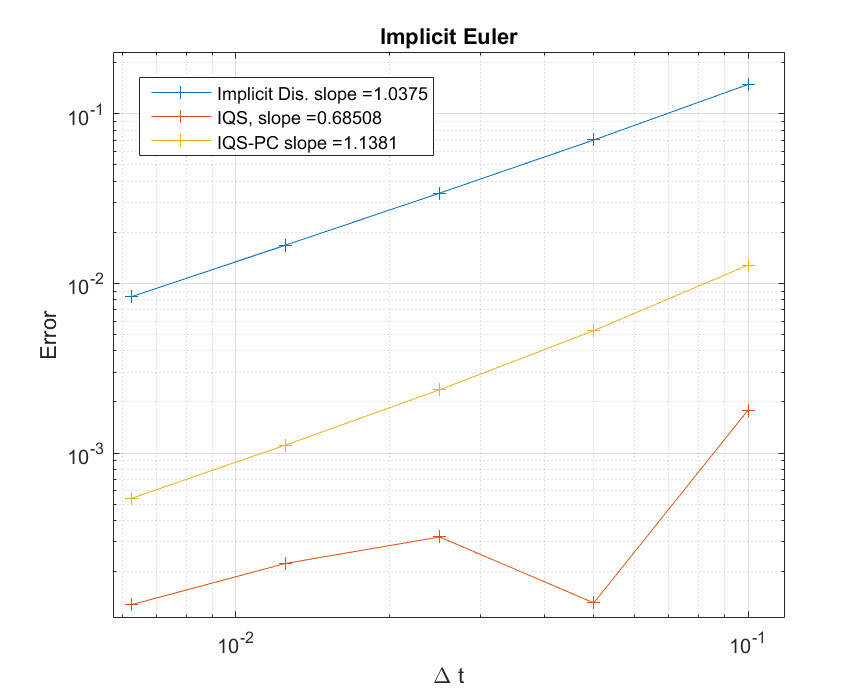
\includegraphics[height=1.5in]{figures/1Dmini_conv_IE.png}
%\caption{Time step convergence for one-dimensional mini-core with implicit Euler discretization}
%\label{fig:1Dmini_conv}
%\end{figure}

%---------------------------------------------------------------------------------------%
\subsection{TWIGL Benchmark}
%---------------------------------------------------------------------------------------%

This benchmark problem originates from the ANL Benchmark Problem Book \cite{ANL_BPB}.  It is a 2D, 2-group reactor core model with no reflector region \cite{TWIGL_benchmark}. The core is smaller (hence the spatial regions are more tightly coupled) and the spatial variation of the flux varies moderately over the transient. Therefore, IQS is expected to perform significantly better than an implicit flux solve. \fig{fig:TWIGL_power} shows the IQS  solution as compared with the implicit flux solution. 
\DIFdelbegin \DIFdel{This illustrates that IQS can yield a much more accurate solution, even at a significantly larger time step than the implicit flux discretization.
}\DIFdelend %DIF > This illustrates that IQS can yield a much more accurate solution, even at a significantly larger time step than the implicit flux discretization.

\begin{figure}[!htbp]
\centering
\begin{subfigure}[!htbp]{0.49\textwidth}
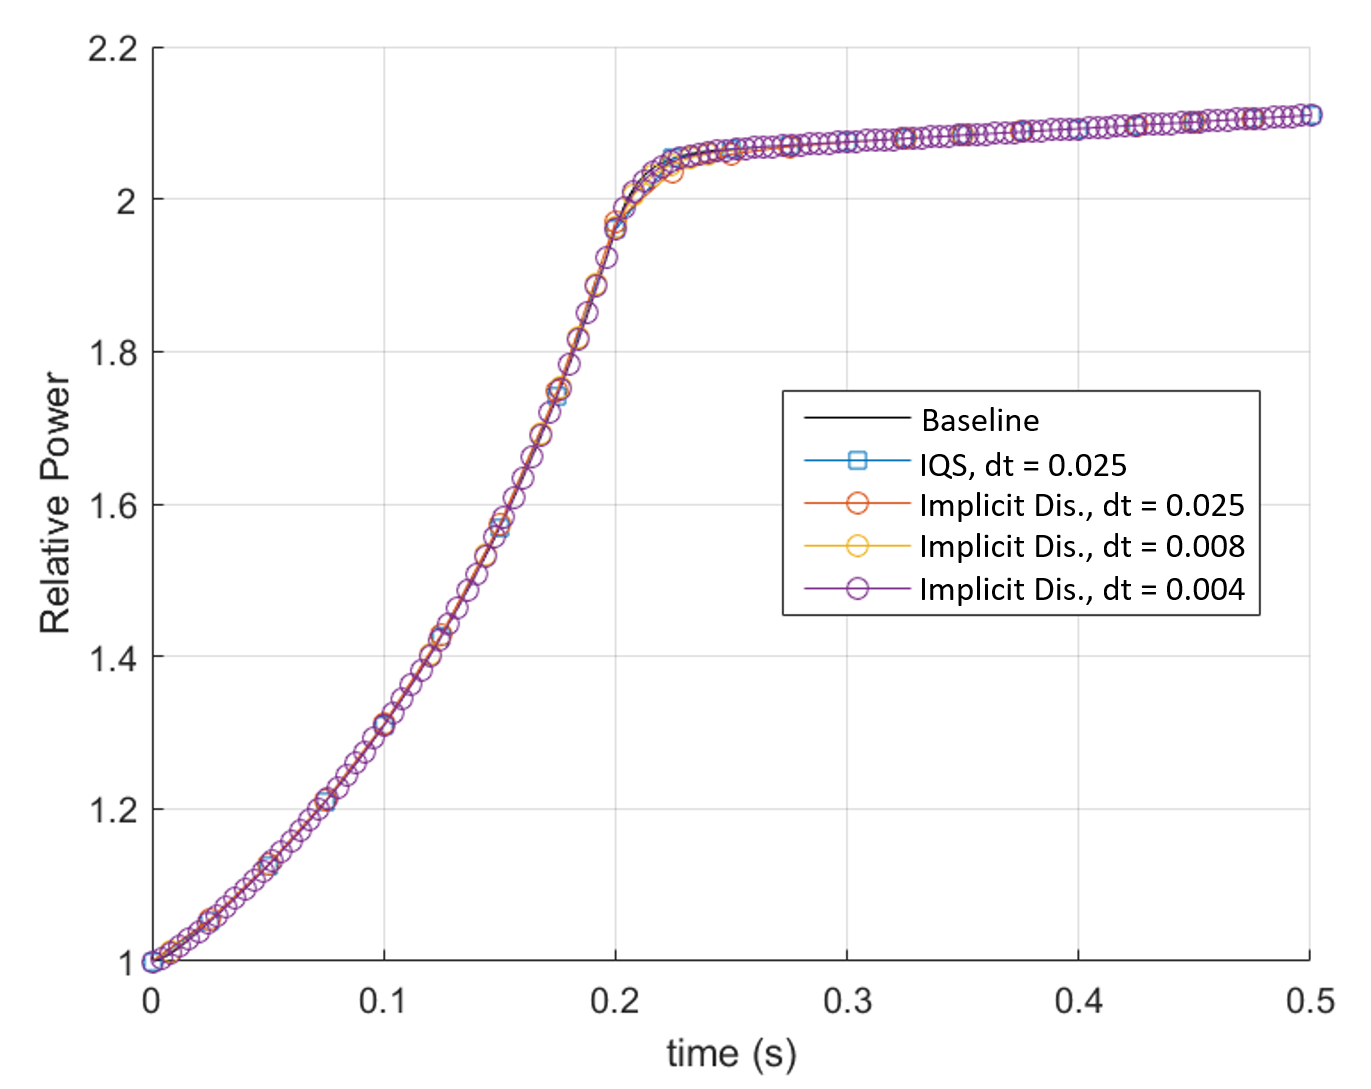
\includegraphics[width=\textwidth]{figures/TWIGL_power_plot.png}
\caption{Power profile for entire transient}
\end{subfigure}
\begin{subfigure}[!htbp]{0.49\textwidth}
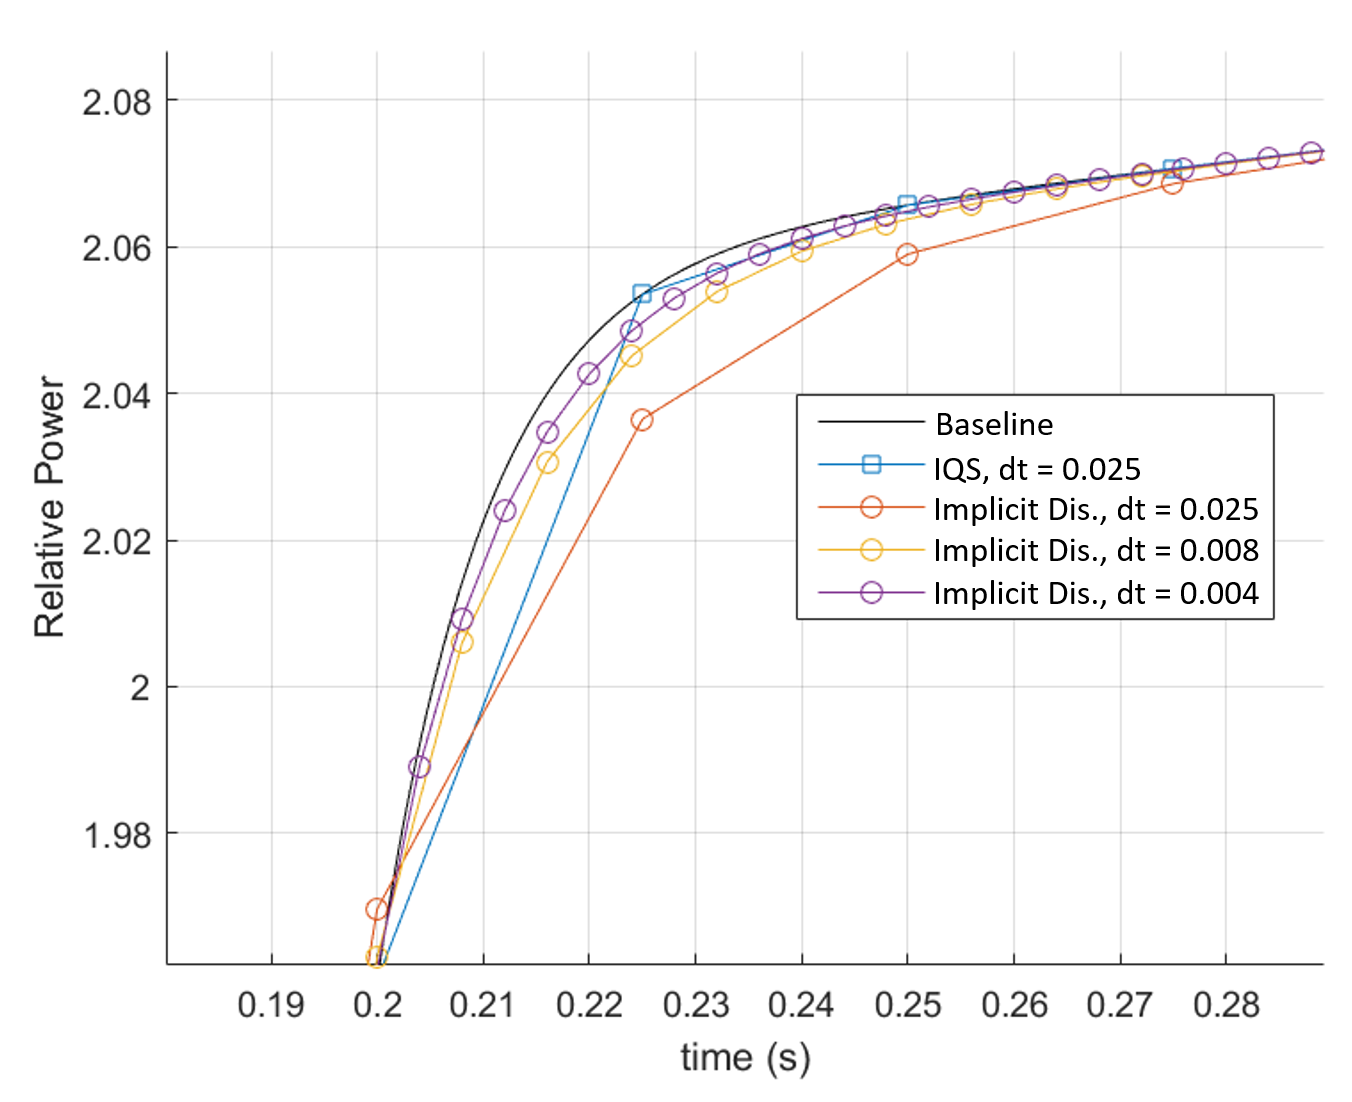
\includegraphics[width=\textwidth]{figures/TWIGL_power_plot2.png}
\caption{Power at cusp of profile}
\end{subfigure}
\caption{Power level comparison of TWIGL Benchmark}
\label{fig:TWIGL_power}
\end{figure}

%----------------------------------------------------------------------------------------
%\subsubsection{TWIGL Time Step Convergence Analysis}

In order to demonstrate asymptotic convergence of IQS, implicit Euler (IE) and second order BDF (BDF2) were applied to solve the TWIGL problem. \fig{fig:TWIGL_conv} plots the error convergence of IQS and the implicit discretization methods.  The curves show the superior convergence of IQS. The observed convergence rates are indicated in the legend. They show orders 1 for IE and 2 for BDF2 for the flux solves. However, the convergence rates for IQS show higher values, order 2 for IE solves for the shape, and above 2.5 for BDF2 solve of the shape. When there is moderate variation in the shape over the transient, the PRKE parameters are accurately estimated, and the fine-scale PRKE solve provides a well resolved amplitude solution.
\DIFaddbegin \DIFadd{The baseline was computed using the BDF2 scheme on the flux equation with a time step of $10^{-5}$. The proper error convergences show that this solution is accurate enough to compare to for error computation for most of the convergence data points. The smallest time step scheme for IQS shows a break in the linearity of the convergence.
These convergence results are consistent with the hypothesis that the performance of IQS is highly dependent on the spatial coupling of the flux.
}\DIFaddend 

\begin{figure}[!htbp]
\centering
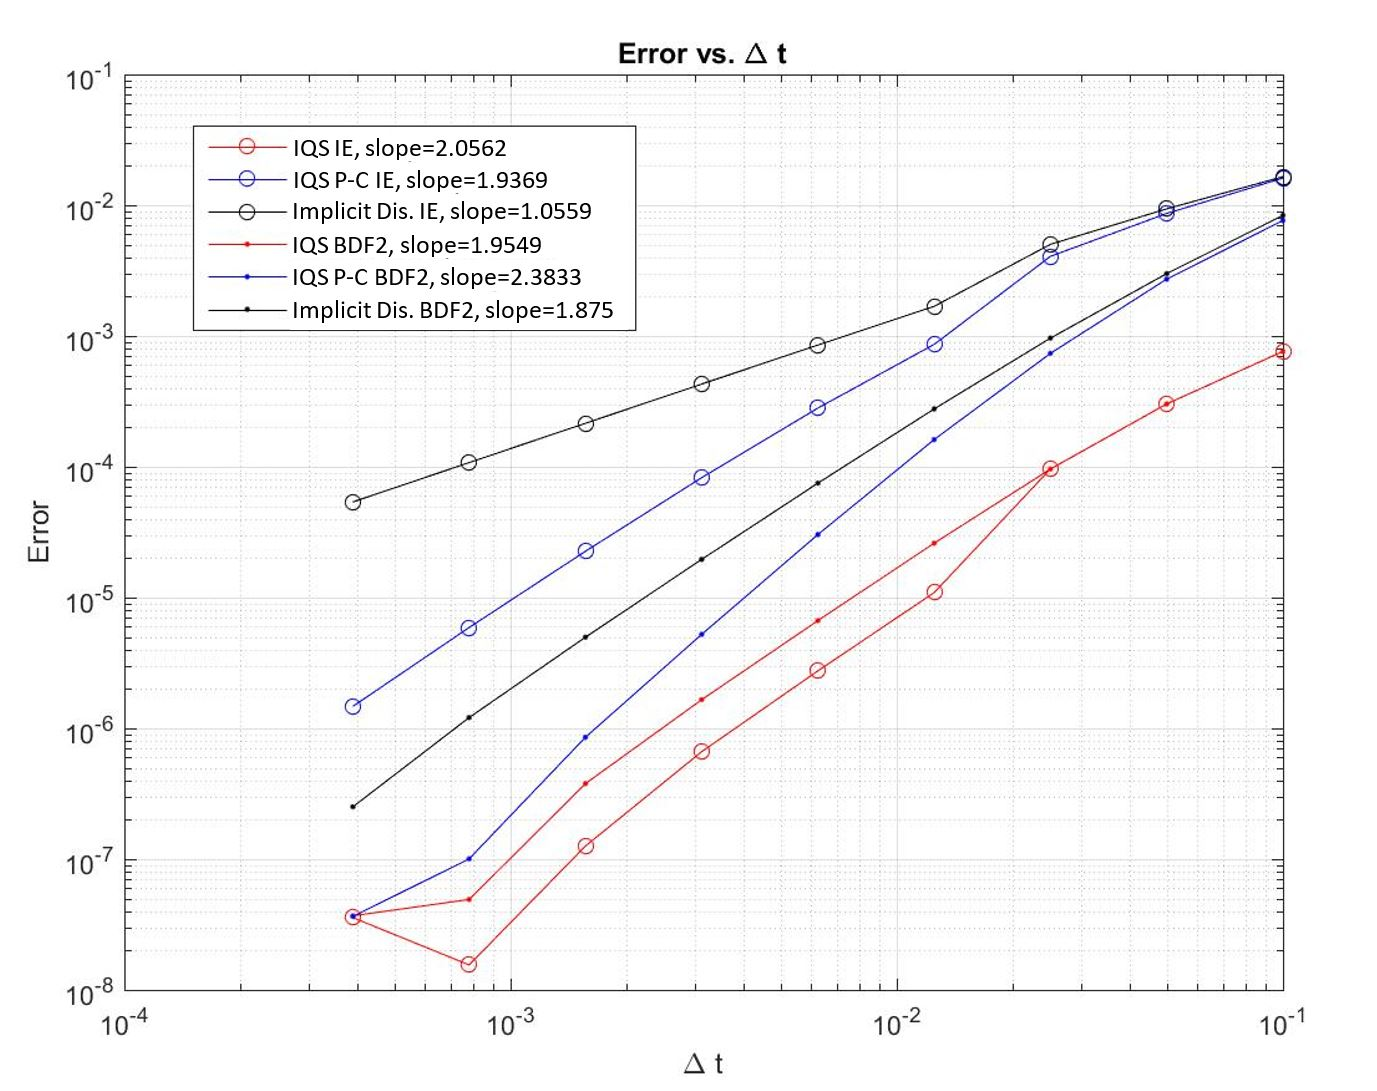
\includegraphics[height=3in]{figures/TWIGL_convergence.jpg}
\caption{Error convergence comparison of TWIGL Benchmark\DIFaddbeginFL \DIFaddFL{. Errors correspond to the relative difference of the power at $t=0.2 s$ from the baseline solution.}\DIFaddendFL }
\label{fig:TWIGL_conv}
\end{figure}

%----------------------------------------------------------------------------------------
%\subsubsection{TWIGL Time Adaptation}

\tbl{tab:TWIGLdt2} and \fig{fig:TWIGL_power_dt2} show the results for the TWIGL benchmark with time adaptation.  The results show that both IQS methods perform exceptionally well compared to implicit flux discretization.  It also shows that traditional IQS performed better with large $e_{tol}$, while \iqspc was better with smaller $e_{tol}$.
\DIFaddbegin \DIFadd{This observation implies that the time adaptive options must be chosen differently when applied to a solver for shape versus a solver for flux.
}\DIFaddend 

\begin{table*}[!htbp]
\begin{center}
\caption{TWIGL step doubling results}
\label{tab:TWIGLdt2}
\DIFdelbeginFL %DIFDELCMD < \resizebox{\linewidth}{!}{
%DIFDELCMD < \begin{tabular}{|l|l|l|l|l|l|l|l|l|l|l|}
%DIFDELCMD < \hline
%DIFDELCMD <   &  & \multicolumn{3}{|c|}{Implicit Discretization} & \multicolumn{3}{|c|}{IQS} & \multicolumn{3}{|c|}{\iqspc} \\
%DIFDELCMD < \hline
%DIFDELCMD < Test & $e_{tol}$ & Error & Steps & Solves & Error & Steps & Solves & Error & Steps & Solves \\
%DIFDELCMD < \hline
%DIFDELCMD < 1 &	0.05    &	0.00012677 &	9   &	29  &	0.03380433 &	4   &	20   &	0.00323100 &	4  &	9   \\
%DIFDELCMD < 2 &	0.01    &	3.5555e-05 &	11  &	35  &	0.00166991 &	5   &	40   &	0.00263068 &	5  &	12  \\
%DIFDELCMD < 3 &	0.005   &	4.0364e-05 &	11  &	31  &	0.00886584 &	5   &	40   &	0.00160486 &	6  &	21  \\
%DIFDELCMD < 4 &	0.001   &	0.00294822 &	33  &	122 &	0.02976305 &	5   &	36   &	1.7527e-05 &	10 &	35  \\
%DIFDELCMD < 5 &	0.0005  &	0.00099778 &	39  &	131 &	0.00143781 &	6   &	55   &	1.4185e-05 &	16 &	74  \\
%DIFDELCMD < 6 &	0.0001  &	0.00019510 &	78  &	236 &	0.00016175 &	8   &	65   &	6.2903e-06 &	19 &	78  \\
%DIFDELCMD < 7 &	5.0e-05 &	0.00018372 &	112 &	342 &	6.0328e-05 &	12  &	163  &	1.5247e-06 &	24 &	92  \\
%DIFDELCMD < % 8 &	1.0e-05 &	8.0564e-05 &	263 &	794 &	7.7103e-05 &	379 &	5729 &	9.8321e-07 &	48 &	210 \\
%DIFDELCMD < \hline
%DIFDELCMD < 

%DIFDELCMD < \end{tabular}}
%DIFDELCMD < %%%
\DIFdelendFL \DIFaddbeginFL \resizebox{\linewidth}{!}{
\begin{tabular}{|l|l|l|l|l|l|l|l|l|l|l|}
\hline
  &  & \multicolumn{3}{|c|}{Implicit Discretization} & \multicolumn{3}{|c|}{IQS} & \multicolumn{3}{|c|}{\iqspc} \\
\hline
Test & $e_{tol}$ & Error$^*$ & Steps & Solves & Error$^*$ & Steps & Solves & Error$^*$ & Steps & Solves \\
\hline
1 &	0.05    &	0.00012677 &	9   &	29  &	0.03380433 &	4   &	20   &	0.00323100 &	4  &	9   \\
2 &	0.01    &	3.5555e-05 &	11  &	35  &	0.00166991 &	5   &	40   &	0.00263068 &	5  &	12  \\
3 &	0.005   &	4.0364e-05 &	11  &	31  &	0.00886584 &	5   &	40   &	0.00160486 &	6  &	21  \\
4 &	0.001   &	0.00294822 &	33  &	122 &	0.02976305 &	5   &	36   &	1.7527e-05 &	10 &	35  \\
5 &	0.0005  &	0.00099778 &	39  &	131 &	0.00143781 &	6   &	55   &	1.4185e-05 &	16 &	74  \\
6 &	0.0001  &	0.00019510 &	78  &	236 &	0.00016175 &	8   &	65   &	6.2903e-06 &	19 &	78  \\
7 &	5.0e-05 &	0.00018372 &	112 &	342 &	6.0328e-05 &	12  &	163  &	1.5247e-06 &	24 &	92  \\
% 8 &	1.0e-05 &	8.0564e-05 &	263 &	794 &	7.7103e-05 &	379 &	5729 &	9.8321e-07 &	48 &	210 \\
\hline
\end{tabular}}\\
\footnotesize{$^*$ relative difference of the power at $t=0.2 s$ from the baseline solution}
\DIFaddendFL \end{center}
\end{table*}

\begin{figure}[!htbp]
\centering
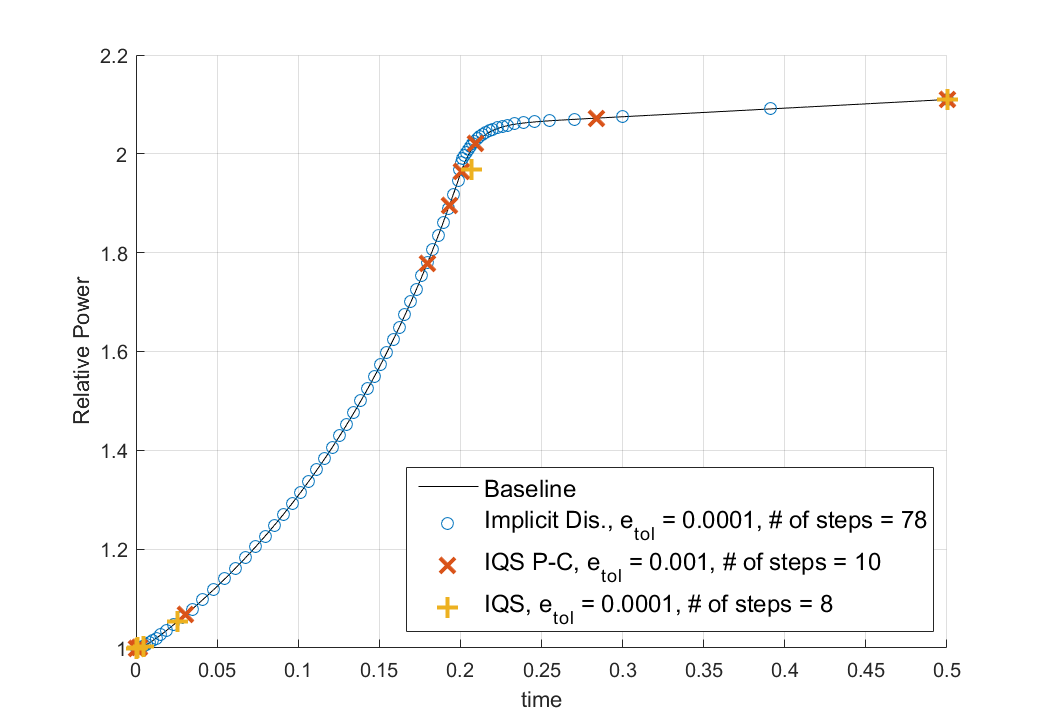
\includegraphics[height=2in]{figures/TWIGL_power_plot_dt2.png}
\caption{Power level comparison of TWIGL Benchmark with time step control}
\label{fig:TWIGL_power_dt2}
\end{figure}

%%%%%%%%%%%%%%%%%%%%%%%%%%%%%%%%%%%%%%%%%%%%%%%%%%%%%%%%%%%%%%%%%%%%%%%%%%%%%%%%%%%%%%%%%
\section{Multiphysics Results}
%%%%%%%%%%%%%%%%%%%%%%%%%%%%%%%%%%%%%%%%%%%%%%%%%%%%%%%%%%%%%%%%%%%%%%%%%%%%%%%%%%%%%%%%%

This section describes two transient multiphysics examples with adiabatic heat-up and Doppler feedback in a thermal reactor: the LRA benchmark from the  ANL Benchmark Problem Book \cite{ANL_BPB} 
and a modelisation of an experiment carried out at the Transient Reactor Test Facility, TREAT \cite{mammoth, Tran15}. 
Both examples were performed using the Rattlesnake/MOOSE framework at INL. The spatial discretization uses continuous finite elements with first-order Lagrangian basis functions.
\DIFaddbegin \DIFadd{Note that any instance of $\Delta t$ in the following figures and commentary signifies the size of the macro time step.
}\DIFaddend 

%---------------------------------------------------------------------------------------%
\subsection{LRA Benchmark}
%---------------------------------------------------------------------------------------%

The LRA benchmark is a two-dimensional, two-group neutron diffusion problem.  
It is a super prompt-critical transient. The \DIFaddbegin \DIFadd{equations being solved are explicitly defined in problem 14-A1 of the ANL Benchmark Problem Book \mbox{%DIFAUXCMD
\cite{ANL_BPB}}%DIFAUXCMD
. The }\DIFaddend execution of the benchmark was performed by the Rattlesnake/MOOSE framework at Idaho National Laboratory (INL) \DIFdelbegin \DIFdel{\mbox{%DIFAUXCMD
\cite{wang2013}}%DIFAUXCMD
}\DIFdelend \DIFaddbegin \DIFadd{\mbox{%DIFAUXCMD
\cite{Rattlesnake_user}}%DIFAUXCMD
}\DIFaddend .  The spatial discretization uses continuous finite elements with first-order Lagrangian basis functions. The mesh consists of blocks $11\times 11$ with five uniform refinements, totaling \DIFdelbegin \DIFdel{$165,165$ }\DIFdelend \DIFaddbegin \DIFadd{$123,904$ }\DIFaddend elements and $124,609$ nodes. Three different temporal solution techniques are used: implicit discretization of the flux equations, IQS formulation, and \iqspc. Crank-Nicolson time discretization scheme is used for the space-time equations. 
\DIFdelbegin \DIFdel{The performance of IQS with temperature feedback is assessed by comparing the solution accuracy at peak power.
}\DIFdelend %DIF > The performance of IQS with temperature feedback is assessed by comparing the solution accuracy at peak power.

\fig{fig:lra_profile} shows the baseline power and temperature transient profile for the LRA benchmark. The baseline results are compared to the results achieved by Sutton and Aviles in \cite{Sutton_1996} and presented in \tbl{tab:base}.  The relative difference in the magnitude of the peak power ($t\approx1.44 s$) from the baseline was used for error comparison.  

\begin{figure}[htbp!]
\centering
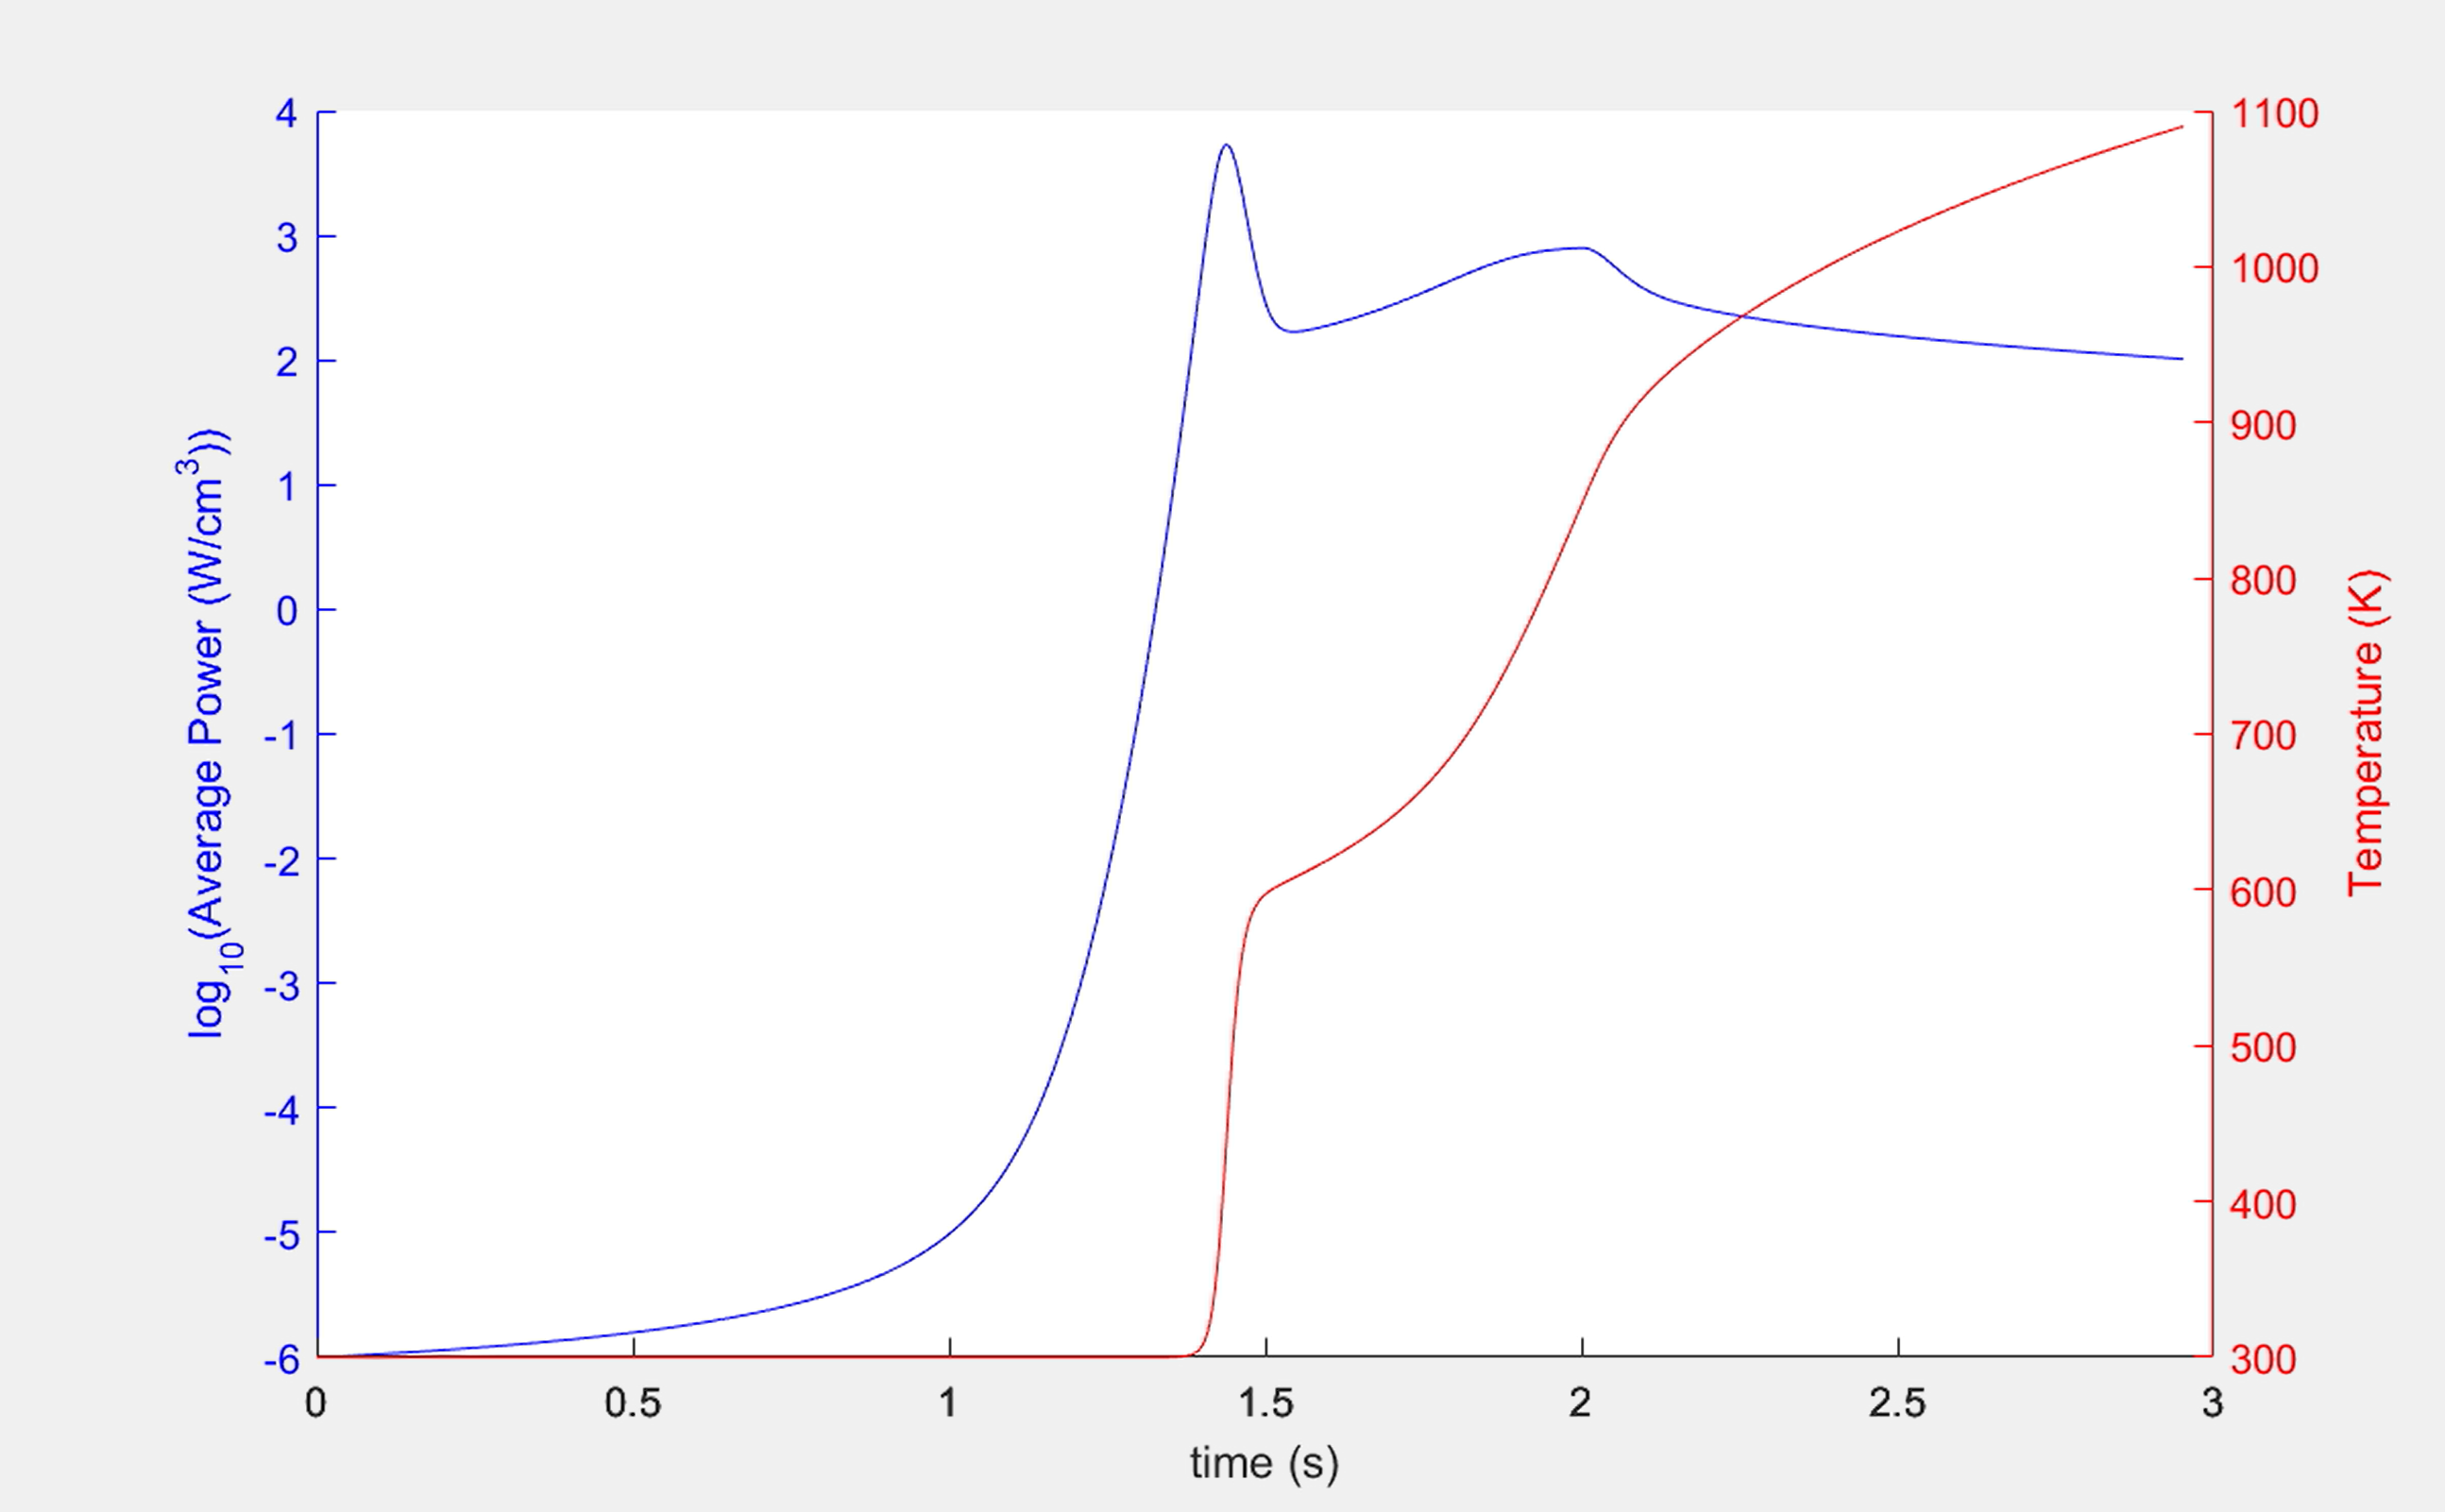
\includegraphics[width=\linewidth]{figures/lra_profile.png}
\caption{LRA baseline temperature and power profile}
\label{fig:lra_profile}
\end{figure}

\begin{table}[!htbp]
\begin{center}
\caption{LRA baseline verification}
\label{tab:base}
%\resizebox{\linewidth}{!}{
\begin{tabular}{|l||c|c|}
\hline
Calculation   &  Baseline Rattlesnake & Sutton (Spandex 1936) \\
\hline\hline
No. of Spatial Nodes	& \DIFdelbeginFL \DIFdelFL{3872 		}\DIFdelendFL \DIFaddbeginFL \DIFaddFL{3,872 		}\DIFaddendFL & \DIFdelbeginFL \DIFdelFL{1936 }\DIFdelendFL \DIFaddbeginFL \DIFaddFL{1,936 }\DIFaddendFL \\
Eigenvalue 				& 0.99637	& 0.99637 \\
No. of Time Steps 		& \DIFdelbeginFL \DIFdelFL{6000 		}\DIFdelendFL \DIFaddbeginFL \DIFaddFL{6,000 		}\DIFaddendFL & 23,890 \\
Time to Peak Power (s) 	& 1.441 	& 1.441 \\
Peak Power (W/cm$^3$) 	& \DIFdelbeginFL \DIFdelFL{5456 		}\DIFdelendFL \DIFaddbeginFL \DIFaddFL{5,456 		}\DIFaddendFL & \DIFdelbeginFL \DIFdelFL{5461 }\DIFdelendFL \DIFaddbeginFL \DIFaddFL{5,461 }\DIFaddendFL \\
\hline
\end{tabular}
%}
\end{center}
\end{table}

%----------------------------------------------------------------------------------------
\subsubsection{IQS Results for the LRA Benchmark without Time Adaptivity}

This section shows the time step error convergence of IQS for the LRA benchmark, as well as the effect of the intermediate temperature time scale. \fig{fig:lra_bad} is an error convergence plot comparing the three \DIFdelbegin \DIFdel{tempoeral }\DIFdelend \DIFaddbegin \DIFadd{temporal }\DIFaddend solution techniques where temperature is evaluated only once per macro step (1 temperature update).  \fig{fig:lra_mpconv} is an error convergence plot comparing the same three techniques when temperature is evaluated 5 times within a macro step (5 temperature updates).  Finally, \fig{fig:mp} shows the effect of various temperature updates. The dashed lines correspond to \DIFaddbegin \DIFadd{the }\DIFaddend implicit flux discretization \DIFdelbegin \DIFdel{at different }\DIFdelend \DIFaddbegin \DIFadd{solutions obtained using different time }\DIFaddend step sizes, while the IQS macro step size is kept constant.

\begin{figure}[!htbp]
\centering
\begin{subfigure}[!htbp]{0.49\textwidth}
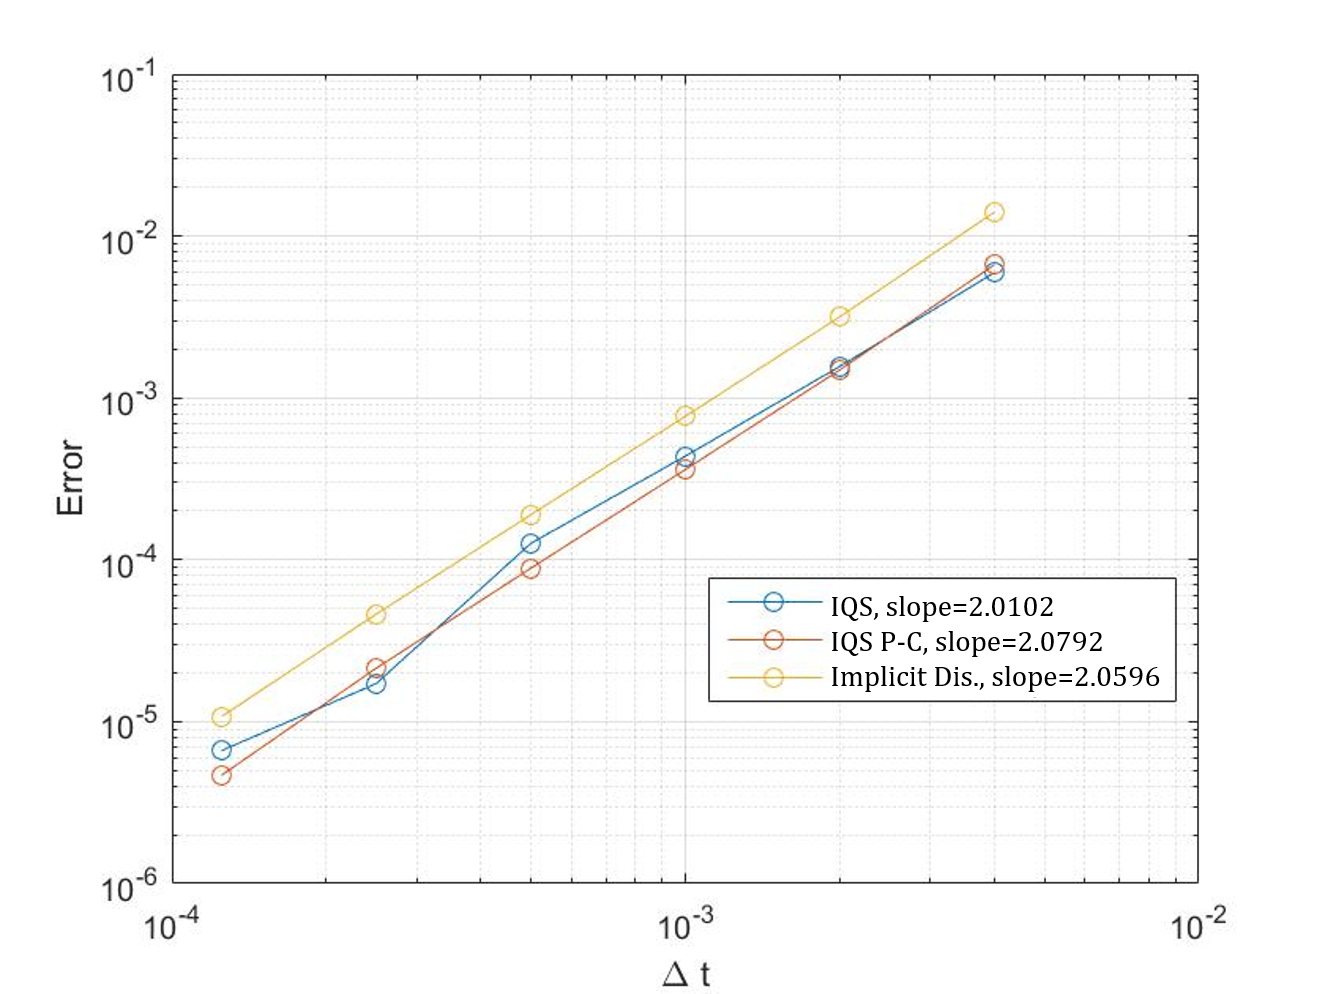
\includegraphics[width=\textwidth]{figures/lra_bad.png}
\caption{Only one temperature update per macro step}
\label{fig:lra_bad}
\end{subfigure}
\begin{subfigure}[!htbp]{0.49\textwidth}
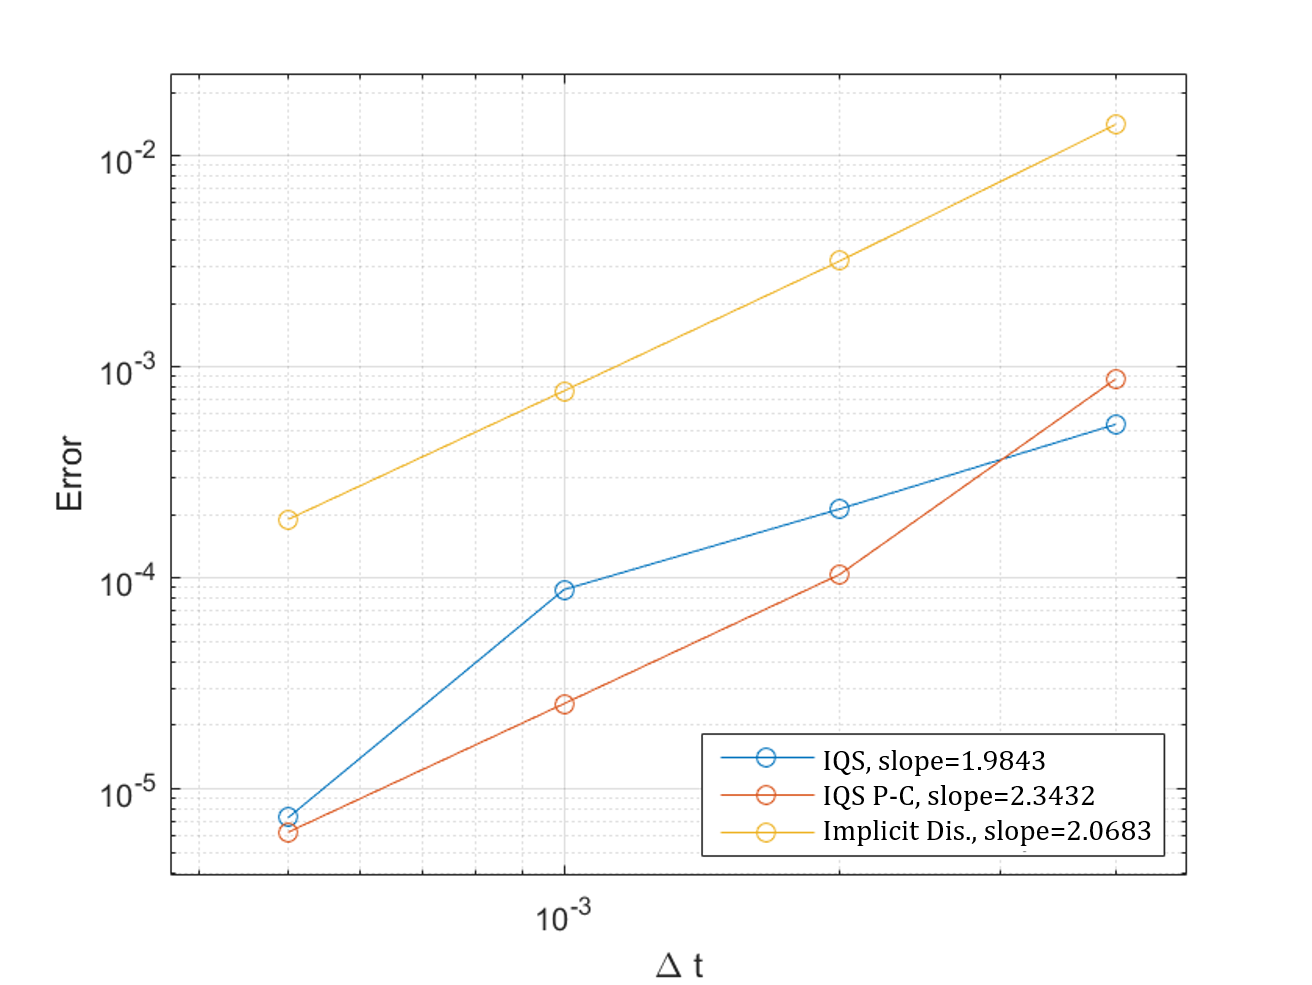
\includegraphics[width=\textwidth]{figures/lra_mp_convergence.png}
\caption{Five temperature updates per macro step}
\label{fig:lra_mpconv}
\end{subfigure}
\caption{LRA error convergence plots}
\end{figure}

\begin{figure}[htbp!]
\centering
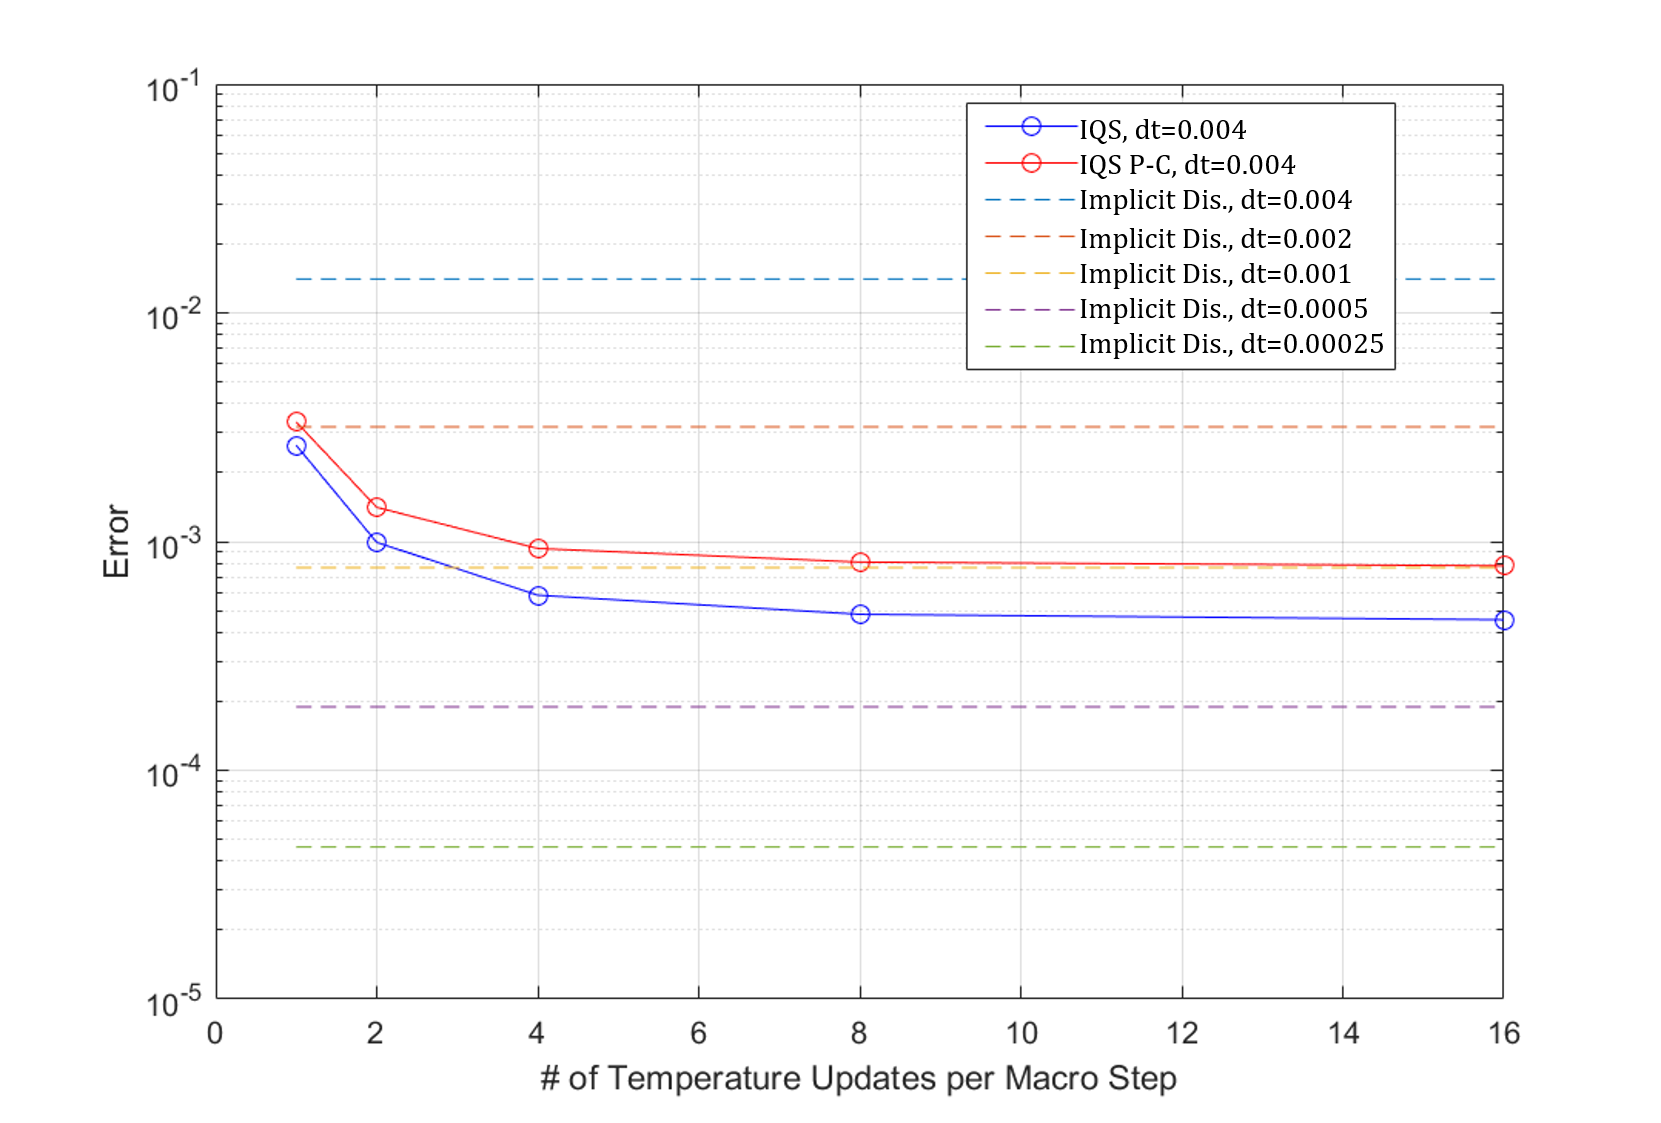
\includegraphics[height=3in]{figures/lra_mp.png}
\caption{Error plot with various temperature updates per macro step}
\label{fig:mp}
\end{figure}

The convergence plots show that updating temperature and the PRKE parameters within a macro step has a significant effect on the performance of IQS.  With only one update, IQS was only slightly better than the implicit flux discretization which required about 50\% more time steps than IQS for the same error.  While 5 temperature updates showed a much improved performance for IQS, with the implicit flux discretization required about 400\% more time steps than IQS for the same error level.  \fig{fig:mp} shows that the solution converges with an increase in the number of temperature updates. 
%
Table \ref{tab:ndiff_lra} shows the run time results for the implicit discretization calculations. The number of GMRES linear iterations is included because it is a proportional measure of the computational effort. Tables \ref{tab:iqs_lra} and \ref{tab:iqspc_lra} present the IQS run-times with various numbers of temperature updates.  These run-times are based on total alive time of the execution where the diffusion evaluation is distributed over 24 processors. These run-times show a marginal performance for IQS and superior performance for \iqspc.  Some of the execution times were able to decrease from implicit discretization with the same number of macro steps because IQS is better equipped to resolve the nonlinearity between temperature and amplitude. Furthermore, there seems to be an optimal number of temperature updates to minimize execution time for a given accuracy.
%: IQS only needs one and \iqspc seems to be ideal at 4 updates. This discrepancy in the number of updates shows that an adaptive type implementation of the updates would be ideal, and could enforce a constant error over the transient. 
It is also important to compare the error of implicit discretization with IQS at one update and \iqspc at 4 updates.  IQS shows an error comparable to implicit discretization at $\Delta t = 0.002$, signifying an actual increase in \DIFdelbegin \DIFdel{runtime }\DIFdelend \DIFaddbegin \DIFadd{run-time }\DIFaddend by -34.1\%.  \iqspc shows an error less than implicit discretization at $\Delta t = 0.002$, signifying an actual increase in \DIFdelbegin \DIFdel{runtime }\DIFdelend \DIFaddbegin \DIFadd{run-time }\DIFaddend by $<-34.9\%$. These specific runs are highlighted in Tables \ref{tab:ndiff_lra} - \ref{tab:iqspc_lra}.
\DIFaddbegin \DIFadd{\fig{fig:lra_rt_vs_err} visualizes the dependence of run-time on error. This figure shows that IQS and }\iqspc \DIFadd{generally have a lower run-time for a certain error than implicit discretization. Furthermore, note that the slopes on the right half of the }\iqspc \DIFadd{runs are shallower than the implicit discretization slope. This shows that by adding more temperature updates, in the 1-4 temperature-updates range, }\iqspc \DIFadd{suffers a lesser increase in run-time for a decrease in error. However, beyond 4 temperature updates, the error in the shape function saturates and no additional benefits can be gained by more frequent temperature updates. 
}\DIFaddend 

\begin{table}[!htbp]
\begin{center}
\caption{Implicit flux discretization run-time results}
\label{tab:ndiff_lra}
\begin{tabular}{|l|l|ccc|}
\hline
Run  &  $\Delta t$ & Error\DIFaddbeginFL \DIFaddFL{$^*$ }\DIFaddendFL & \DIFdelbeginFL \DIFdelFL{Runtime }\DIFdelendFL \DIFaddbeginFL \DIFaddFL{Run-time }\DIFaddendFL (hr) & Linear Iter.\\
\hline
1	& 4.0e-3	& 1.407e-2 	& 4.11	& 7.13e4	\\
\rowcolor{yellow} 2	& 2.0e-3	& 3.174e-3 	& 6.01	& 9.49e4 	\\
3 	& 1.0e-3 	& 7.690e-4 	& 10.38	& 1.45e5	\\
4 	& 5.0e-4 	& 1.892e-4 	& 21.91	& 2.08e5	\\
5 	& 2.5e-4	& 4.590e-5 	& 25.23	& 3.16e5	\\
\hline
\end{tabular} \DIFaddbeginFL \\
\DIFadd{\footnotesize{$^*$ relative difference of the peak power from the baseline solution}}
\DIFaddendFL \end{center}
\end{table}

\begin{table}[!htbp]
\begin{center}
\caption{IQS run-time results with $\Delta t = 0.004$}
\label{tab:iqs_lra}
\begin{tabular}{|l|l|ccc|}
\hline
	&  Temperature 	&  		& \DIFdelbeginFL \DIFdelFL{Runtime 	}\DIFdelendFL \DIFaddbeginFL \DIFaddFL{Run-time 	}\DIFaddendFL & \% Increase	\\
Run	&  Updates 	& Error\DIFaddbeginFL \DIFaddFL{$^*$ }\DIFaddendFL & (hr)		& in \DIFdelbeginFL \DIFdelFL{Runtime$^*$}\DIFdelendFL \DIFaddbeginFL \DIFaddFL{Run-time$^{\dagger}$}\DIFaddendFL \\
\hline
\rowcolor{yellow} 1	& 1		& 2.612e-3 	& 3.96 	& -3.18\%	\\
2	& 2		& 9.893e-4 	& 6.02	&  47.1\%	\\
3 	& 4 	& 5.796e-4 	& 7.87	&  92.3\%	\\
4 	& 8 	& 4.772e-4 	& 12.61	& 207.9\% 	\\
5 	& 16	& 4.516e-4 	& 22.14	& 440.7\%	\\
\hline
\end{tabular}
\\
\DIFadd{\footnotesize{$^*$ relative difference of the peak power from the baseline solution}}\\
\footnotesize{\DIFdel{$^*$}\DIFadd{$^{\dagger}$} difference in run-time from $\Delta t = 0.004$ implicit discretization} 
\end{center}
\end{table}

\begin{table}[!htbp]
\begin{center}
\caption{\iqspc run time results with $\Delta t = 0.004$}
\label{tab:iqspc_lra}
\begin{tabular}{|l|l|ccc|}
\hline
	&  Temperature 	&  		& \DIFdelbeginFL \DIFdelFL{Runtime 	}\DIFdelendFL \DIFaddbeginFL \DIFaddFL{Run-time 	}\DIFaddendFL & \% Increase	\\
Run	&  Updates 	& Error\DIFaddbeginFL \DIFaddFL{$^*$ }\DIFaddendFL & (hr)		& in \DIFdelbeginFL \DIFdelFL{Runtime$^*$}\DIFdelendFL \DIFaddbeginFL \DIFaddFL{Run-time$^{\dagger}$}\DIFaddendFL \\
\hline
1	& 1		& 3.488e-3 	& 2.91 	& -28.9\%	\\
2	& 2		& 1.349e-3 	& 3.73	& -9.00\%	\\
\rowcolor{yellow} 3 	& 4 	& 9.161e-4 	& 3.97	& -3.04\%	\\
4 	& 8 	& 8.052e-4 	& 5.39	&  31.7\%	\\
5 	& 16	& 7.905e-4 	& 8.19	&  100\%	\\
\hline
\end{tabular}
\\
\DIFadd{\footnotesize{$^*$ relative difference of the peak power from the baseline solution}}\\
\footnotesize{\DIFdel{$^*$}\DIFadd{$^{\dagger}$} difference in run-time from $\Delta t = 0.004$ implicit discretization} 
\end{center}
\end{table}

\DIFaddbegin \begin{figure}[htbp!]
\centering
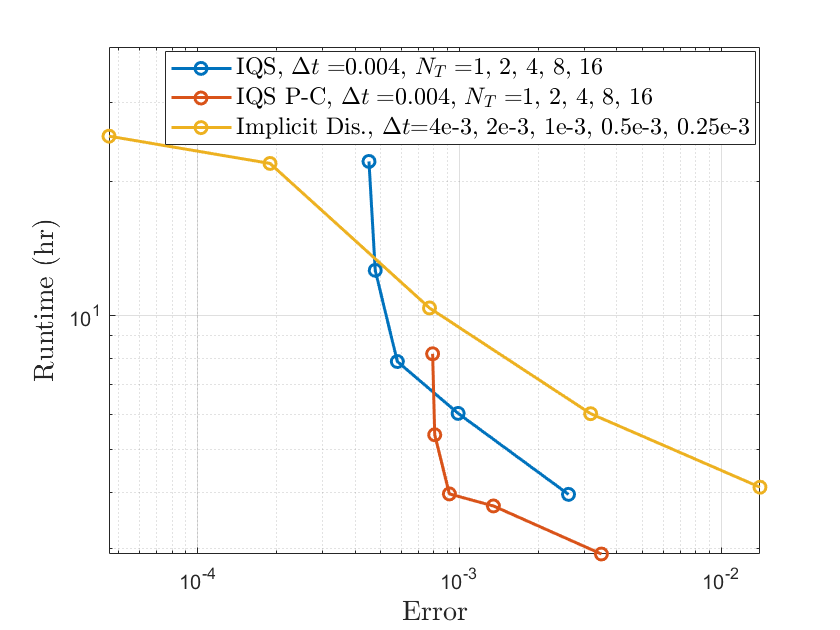
\includegraphics[height=3in]{figures/lra_rt_vs_err.png}
\caption{\DIFaddFL{Run-time vs. error for various number of temperature updates of IQS and }\iqspc\DIFaddFL{, and various time step sizes of Implicit Dis. (lower is better)}}
\label{fig:lra_rt_vs_err}
\end{figure}

\DIFadd{Up to now, errors presented in this section were norms (i.e., space-integrated flux errors). However, for reactor physics problems, it is also noteworthy to compare the spatial dependence of error, for example, error in the power distribution. \fig{fig:lra_block} shows the difference in power for each assembly of the LRA geometry for each method. The resulting spatially dependent error is in general an order of magnitude lower for IQS and }\iqspc \DIFadd{than for the implicit flux discretization. This observation agrees well with the integrated flux errors shown in Tables \ref{tab:ndiff_lra}-\ref{tab:iqspc_lra}. 
}

\begin{figure}[htbp!]
\centering
\resizebox{\textwidth}{!}{%
\begin{tikzpicture}[every node/.style = {font=\normalsize}]

\node[inner sep=0pt, anchor=south](fig) at (0,0) {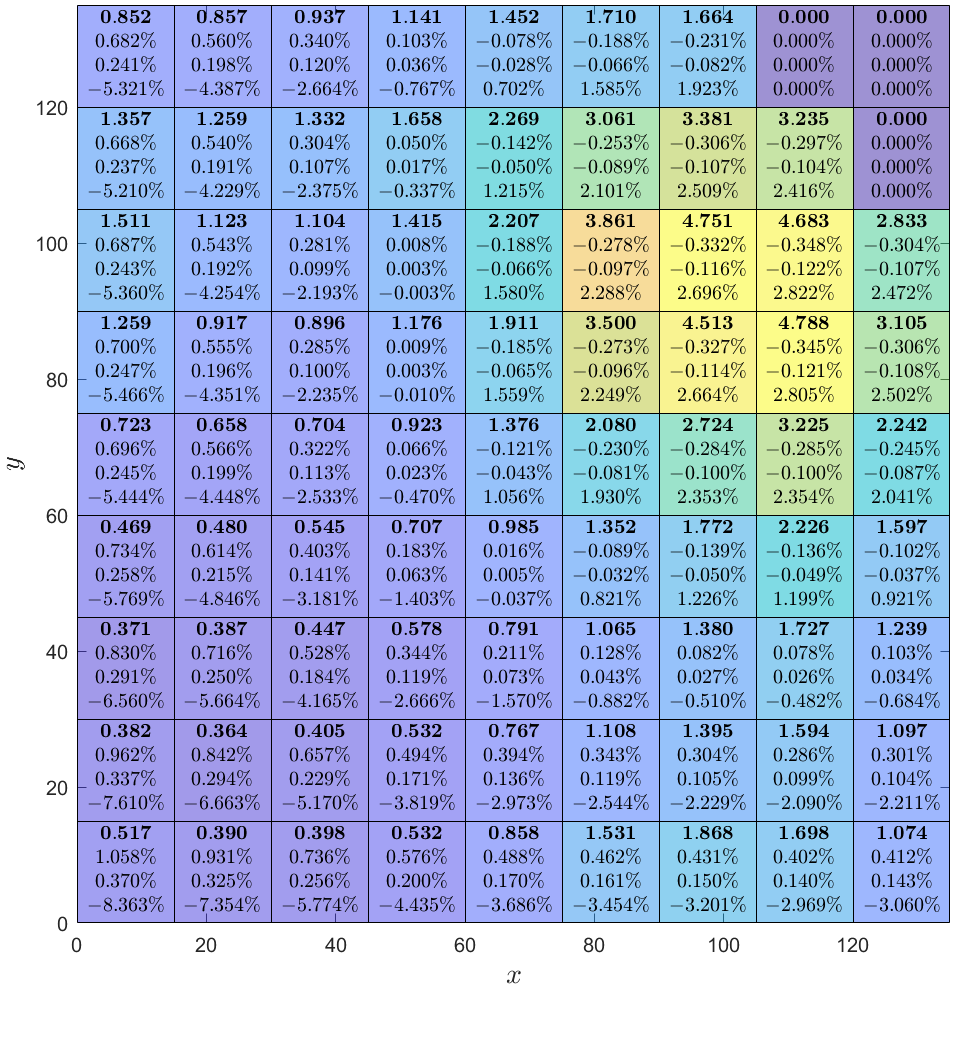
\includegraphics[height=5in]{figures/lra_block.png}};
\node[rectangle, draw, align=center,anchor=north east, style={font=\footnotesize}] (des) at (1,0) {\textbf{Normalized Power (Ref.)} \\ Difference (IQS) - $\Delta t = 0.004, \ N_T = 4$ \\ Difference (\iqspc) - $\Delta t = 0.004, \ N_T = 4$ \\ Difference (Implicit Dis.) - $\Delta t = 0.004$};
\node[anchor= north west] (dif) at (1,0) {Difference $= \frac{\text{Power}^\text{ref} - \text{Power}}{\text{Power}^\text{ref}}$};

\end{tikzpicture}%
}
\caption{\DIFaddFL{Difference in normalized power from reference solution for each fissile block of the LRA geometry}}
\label{fig:lra_block}
\end{figure}


\DIFaddend %----------------------------------------------------------------------------------------
\subsubsection{IQS Results for the LRA Benchmark with Time Adaptivity}

\fig{fig:lra_dt2} shows the power profile of the LRA \DIFdelbegin \DIFdel{with time a of }\DIFdelend \DIFaddbegin \DIFadd{while using time adaptivity for }\DIFaddend implicit discretization and \iqspc\DIFdelbegin \DIFdel{, and \tbl{tab:lra_dt2} compiles the }\DIFdelend \DIFaddbegin \DIFadd{; \tbl{tab:lra_dt2} compiles these }\DIFaddend results. These adaptivity results show the significant decrease in the number of macro time steps required for \iqspc. The power profiles were obtaining with only one temperature update per macro step.

\begin{figure}[!htbp]
\centering
\begin{subfigure}[!htbp]{0.49\textwidth}
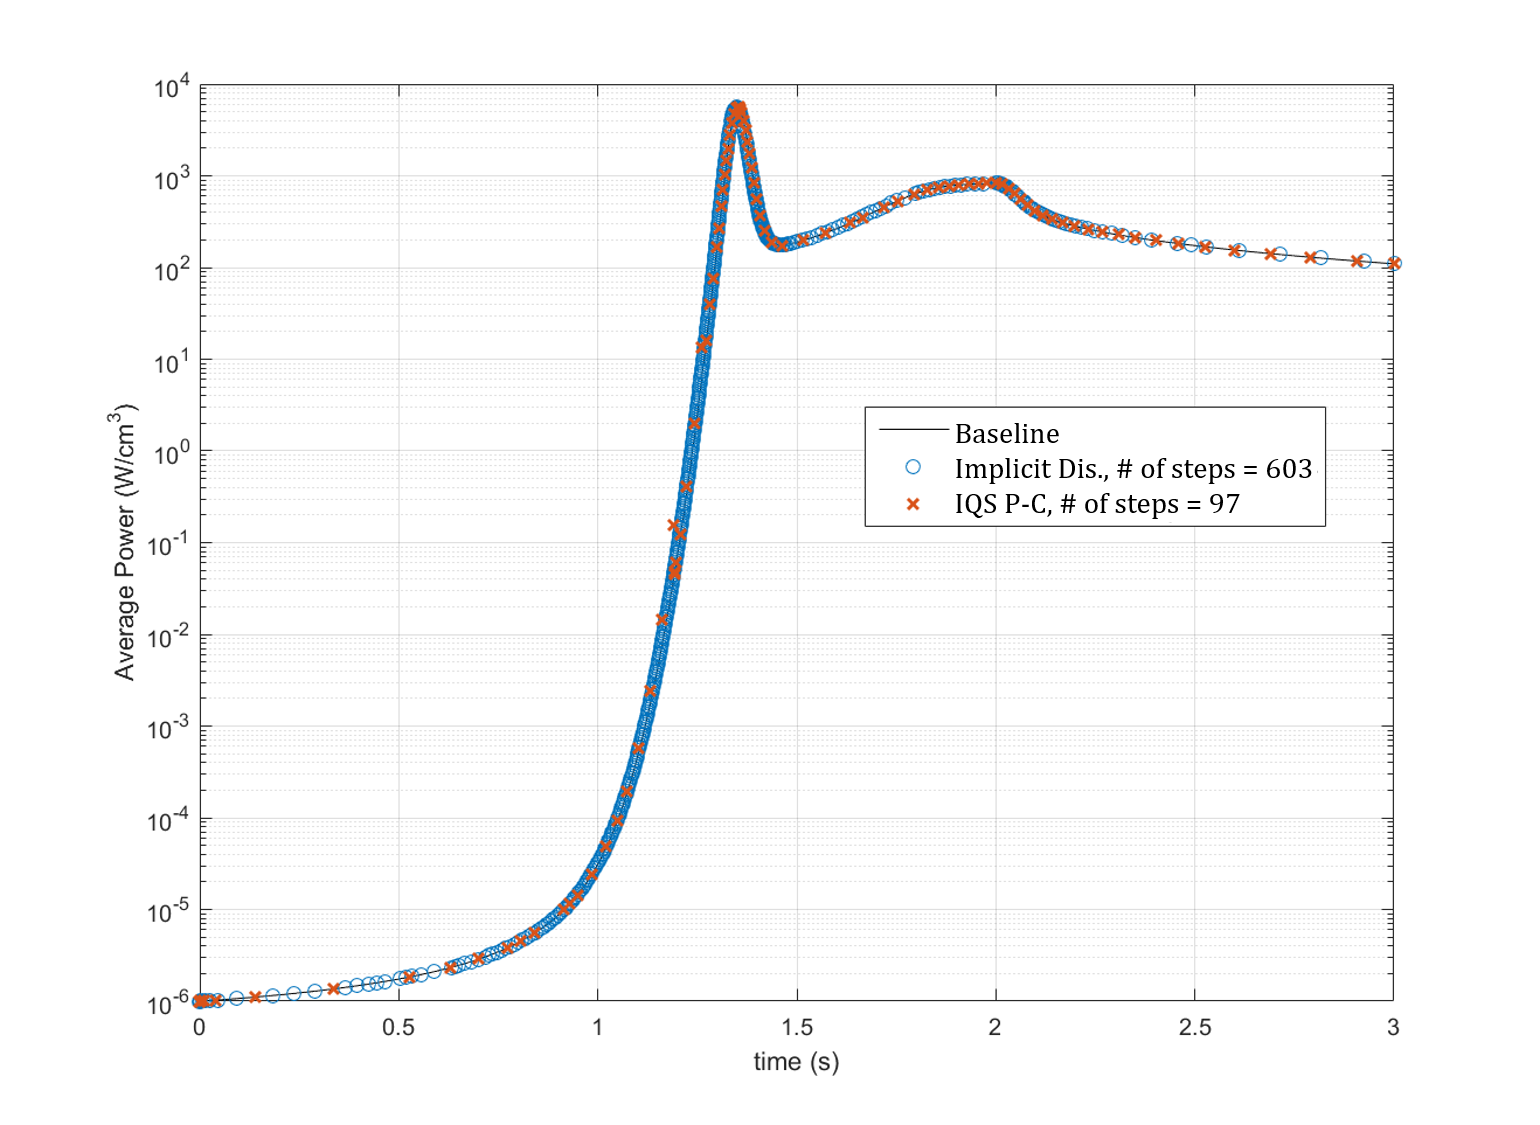
\includegraphics[width=\textwidth]{figures/LRA_DT2.png}
\caption{Full power profile}
\end{subfigure}
\begin{subfigure}[!htbp]{0.49\textwidth}
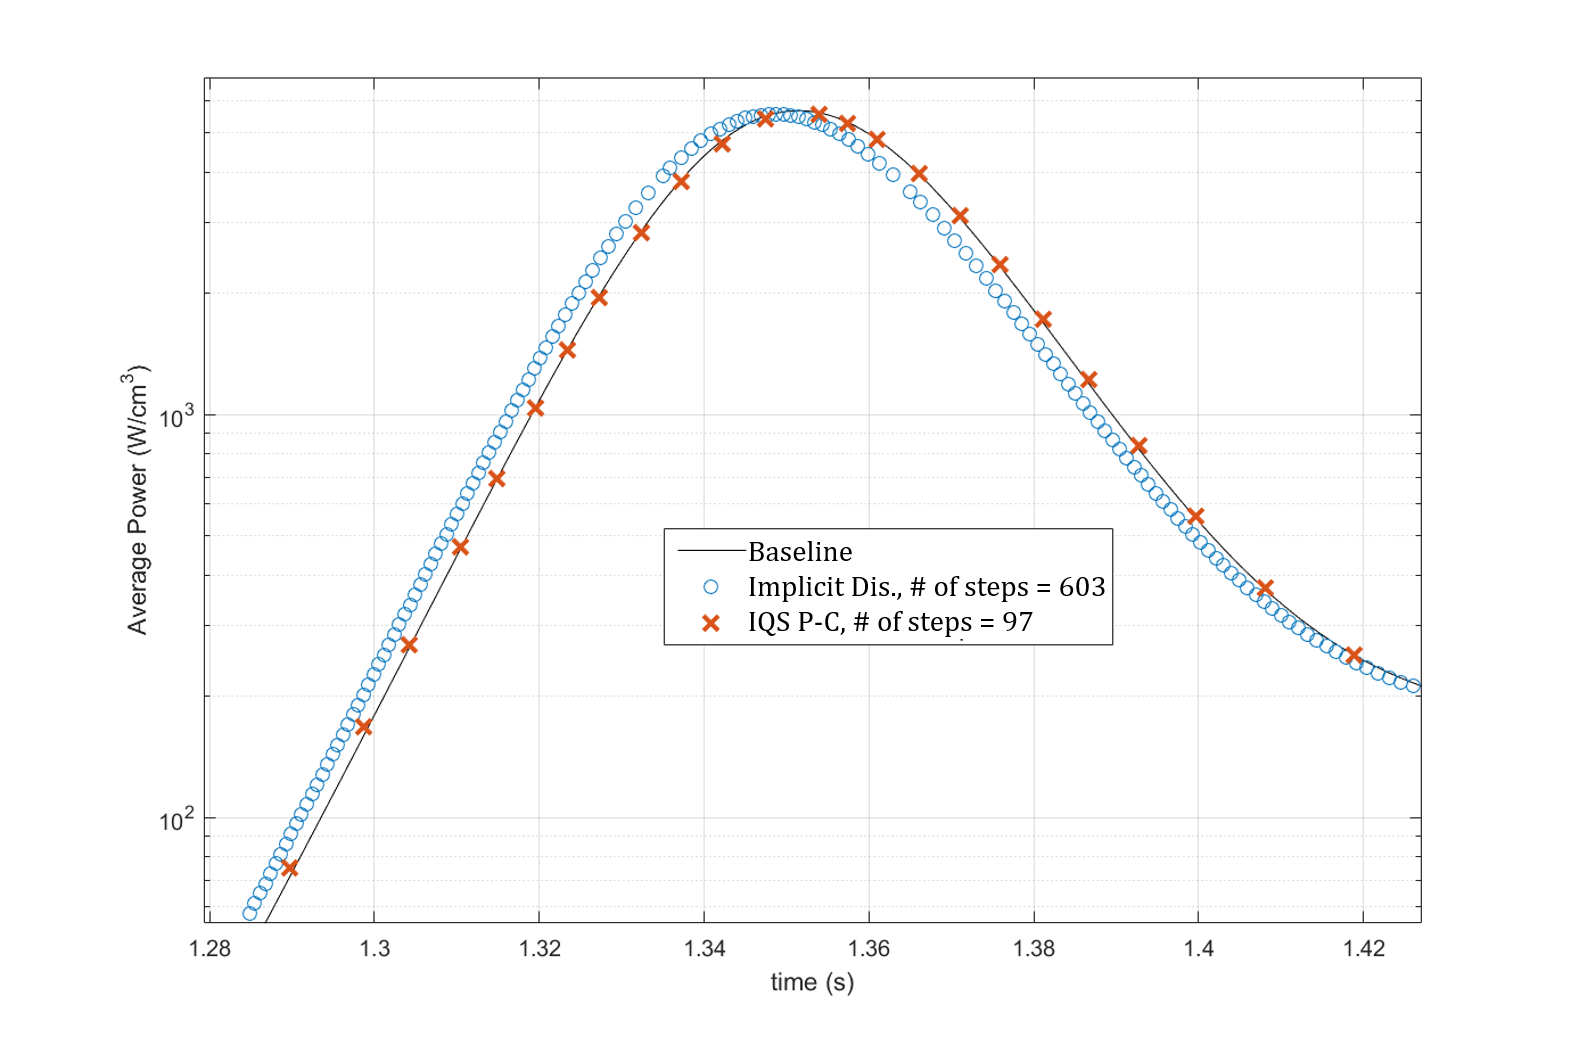
\includegraphics[width=\textwidth]{figures/LRA_DT2_peak.png}
\caption{Peak power profile at peak}
\end{subfigure}
\caption{LRA power profile with time adaptation of implicit discretization and \iqspc}
\label{fig:lra_dt2}
\end{figure}

\begin{table}
\begin{center}
\caption{LRA step doubling adaptation results with implicit discretization and \iqspc}
\label{tab:lra_dt2}
\resizebox{\linewidth}{!}{
\begin{tabular}{|l|l|l|l|l|l|l|}
\hline
 & \multicolumn{3}{|c|}{Implicit Dis.} & \multicolumn{3}{|c|}{\iqspc} \\
\hline
Event & Power & Error & Steps & Power  & Error & Steps \\
 & (W/cm$^3$) &  &  &  (W/cm$^3$) &  &  \\
\hline
Max Power & 5567.3 & 0.019454 & 423 & 5568.3 & 0.019274 & 47 \\
End (3 s) & 109.66 & 2.3650e-4 & 603 & 109.65 & 3.0622e-4 & 97 \\
\hline
\end{tabular}}
\end{center}
\end{table}

%---------------------------------------------------------------------------------------%
\subsection{TREAT Transient-15 Problem}
%---------------------------------------------------------------------------------------%

Transient-15 is a test case based on the TREAT core at the INL \cite{mammoth, Tran15}. 
This test case is not meant to model an actual TREAT experiment but was created to evaluate Rattlesnake’s physics 
models for TREAT transient with feedback.  However, the model was complex enough and representative enough to test 
the performance of IQS and its time scale based treatment of temperature. Transient-15 involves an 11-energy group diffusion approximation and the geometry is discretized into $355,712$ hexahedral continuous finite elements totaling $4,109,523$ degrees of freedom.  The three-second transient involves a linear ramp decrease in the absorption cross section throughout the control rod region (to simulate a rod movement out of the core). \fig{fig:Tran15} shows a visualization of the flux profile within the core (the graphite reflector has been removed in the picture to show only the active core).   

\begin{figure}[htbp!]
\centering
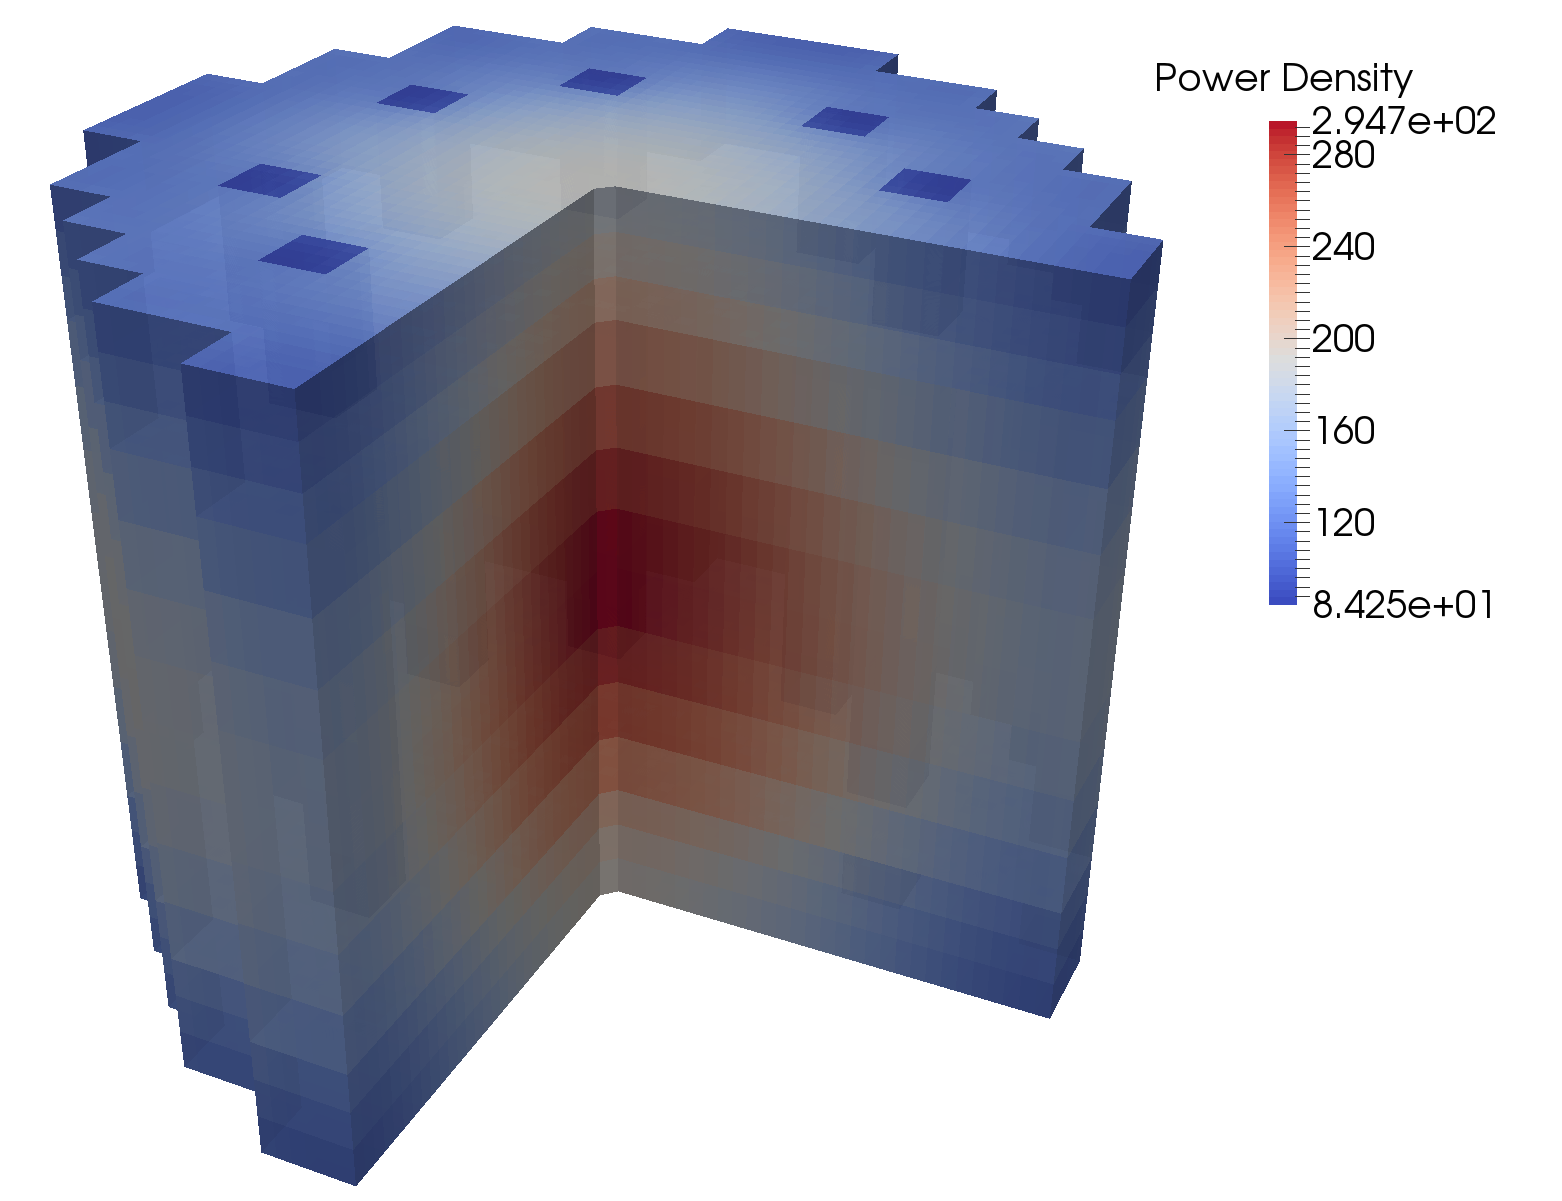
\includegraphics[height=2.5in]{figures/Tran15_core2.png}
\caption{Transient-15 core power profile at peak power ($t=1.90 s$)}
\label{fig:Tran15}
\end{figure}

The Transient-15 model uses an adiabatic temperature feedback mechanism, similar to the one used in the LRA benchmark \DIFdelbegin \DIFdel{.
\eqt{eq:temp2} describes the heat up of the fuel, where, }\DIFdelend \DIFaddbegin \DIFadd{(see, Eq.~}\eqref{eq:temp}\DIFadd{, except }\DIFaddend this time, the fuel specific heat capacity is itself also temperature-dependent\DIFaddbegin \DIFadd{)}\DIFaddend . Hence, the temperature evaluation is identical to the one described in LRA section, except a Newton iteration process is employed to resolve the nonlinearity from the specific heat \DIFaddbegin \DIFadd{capacity }\DIFaddend term.  The 11-g neutron cross sections are linearly interpolated at tabulated temperatures.
\DIFdelbegin %DIFDELCMD < 

%DIFDELCMD < \be
%DIFDELCMD < %%%
\tcr{
\be
\DIFdel{\rho c_p(T) \frac{\partial T(\vec{r},t)}{\partial t} = \kappa_f \sum^G_{g=1}\Sigma_f^g \phi^g(\vec{r},t)}
\label{eq:temp2}
\ee
}
\addtocounter{equation}{-1}
\DIFdelend %DIF > 
%\be
%c_p = -5.8219e-10T^3 - 4.3694e-7T^2 + 2.8369e-3T -1.009e-2
%\label{eq:cp}
%\ee

%----------------------------------------------------------------------------------------
%\subsubsection{Transient-15 Multiphysics Time Scale Results}

In order to test the temperature feedback treatment, six different scenarios were run: a baseline with a very small time-step, implicit flux discretization, IQS with one and 5 temperature updates per macro step, and \iqspc with one and 5 temperature updates.  \fig{fig:Tran15_profile} shows the baseline power and temperature profile for the Transient-15 example.  \tbl{tab:tran15} shows the error and run-time results.

\begin{figure}[htbp!]
\centering
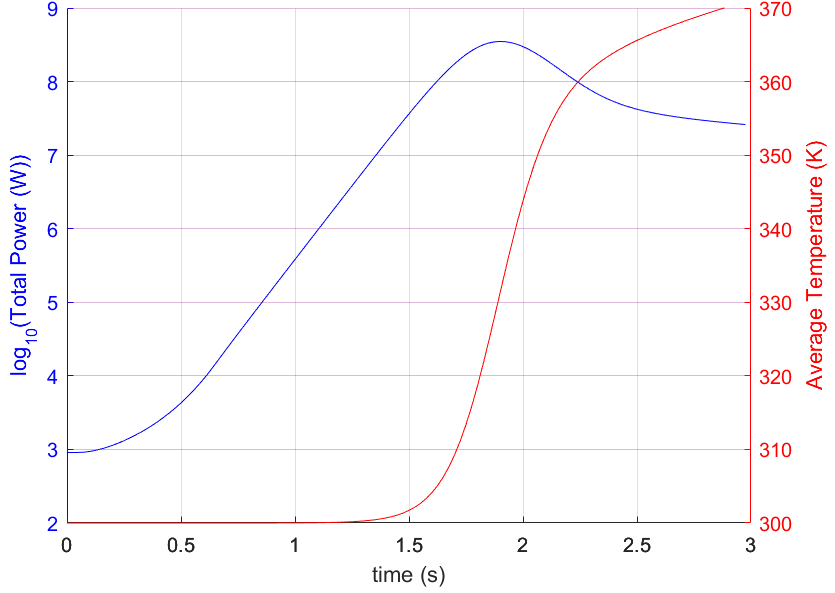
\includegraphics[height=3in]{figures/Tran15_profile.png}
\caption{Transient-15 total power and average temperature profile during transient}
\label{fig:Tran15_profile}
\end{figure}

\begin{table}[htb]
\begin{center}
\DIFdelbeginFL %DIFDELCMD < \resizebox{\linewidth}{!}{
%DIFDELCMD < \begin{tabular}{|l|ccccccc|}
%DIFDELCMD < \hline
%DIFDELCMD <  & No.	& Max &	Time at Max &	Max Average &	\% Increase &	Max Power & Linear	\\
%DIFDELCMD < Method & of Steps &	Power (W) &	Power (s) &	Temperature (K) & Runtime$^*$ & Error & Iterations \\
%DIFDELCMD < \hline
%DIFDELCMD < Baseline 			& 3000 	& 3.5039e+08 & 1.901 & 371 &	---		&	---		 & ---		\\
%DIFDELCMD < Implicit Disc. 		& 300 	& 3.5011e+08 & 1.90  & 371 &	---		&	7.875e-4 & 41020	\\
%DIFDELCMD < IQS 				& 300	& 3.5036e+08 & 1.90  & 371 & -11.9\%	&	8.385e-5 & 23949	\\
%DIFDELCMD < IQS (5 updates) 	& 300 	& 3.5040e+08 & 1.90  & 371 &  49.7\%	&	3.687e-5 & 24035	\\
%DIFDELCMD < \iqspc 			& 300 	& 3.5065e+08 & 1.90  & 371 &  -2.1\%	&	7.527e-4 & 39020	\\
%DIFDELCMD < \iqspc (5 updates) & 300 	& 3.5043e+08 & 1.90  & 371 &  26.5\%	&	1.227e-4 & 37866	\\
%DIFDELCMD < \hline
%DIFDELCMD < \end{tabular}
%DIFDELCMD < }
%DIFDELCMD < %%%
\DIFdelendFL \DIFaddbeginFL \resizebox{\linewidth}{!}{
\begin{tabular}{|l|ccccccc|}
\hline
 & No.	& Max &	Time at Max &	Max Average &	\% Increase &	Max Power & Linear	\\
Method & of Steps &	Power (W) &	Power (s) &	Temperature (K) & Run-time$^*$ & Error & Iterations \\
\hline
Baseline 			& 3000 	& 3.5039e+08 & 1.901 & 371 &	---		&	---		 & ---		\\
Implicit Disc. 		& 300 	& 3.5011e+08 & 1.90  & 371 &	---		&	7.875e-4 & 41020	\\
IQS 				& 300	& 3.5036e+08 & 1.90  & 371 & -11.9\%	&	8.385e-5 & 23949	\\
IQS (5 updates) 	& 300 	& 3.5040e+08 & 1.90  & 371 &  49.7\%	&	3.687e-5 & 24035	\\
\iqspc 			& 300 	& 3.5065e+08 & 1.90  & 371 &  -2.1\%	&	7.527e-4 & 39020	\\
\iqspc (5 updates) & 300 	& 3.5043e+08 & 1.90  & 371 &  26.5\%	&	1.227e-4 & 37866	\\
\hline
\end{tabular}
}
\DIFaddendFL \end{center}
\vspace{-3mm}
$^*$ difference in run-time from implicit discretization 
\caption{Transient-15 Error and \DIFdelbeginFL \DIFdelFL{Runtime }\DIFdelendFL \DIFaddbeginFL \DIFaddFL{Run-time }\DIFaddendFL Results}
\label{tab:tran15}
\end{table}

The results from \tbl{tab:tran15} show similar performance of IQS with the temperature updates as in the LRA
test case. Again, the number of linear GMRES iterations is shown as a measure of computational cost. However, these iterations do not consider the temperature updates (auxiliary kernels solved outside of the GMRES solver for temperature updates). IQS with 1 temperature update shows a performance that reduces the error to approximately a tenth of the implicit flux discretization error, and reduces the execution time by about 12\%.  This shows that IQS was able to resolve the nonlinearity between flux and temperature with significantly fewer diffusion evaluations.  Having IQS with 5 updates increased the execution time for the same time step, but the error was further reduced.  Comparing this error to a similar implicit flux discretization error at a smaller time step could show that the run-time was reduced. \iqspc performed not nearly as well as it did with the LRA benchmark, but still proved to be effective.  Having 5 updates for \iqspc increased the run-time marginally, but decreased the error significantly.


%%%%%%%%%%%%%%%%%%%%%%%%%%%%%%%%%%%%%%%%%%%%%%%%%%%%%%%%%%%%%%%%%%%%%%%%%%%%%%%%%%%%%%%%%
\section{Conclusions}
%%%%%%%%%%%%%%%%%%%%%%%%%%%%%%%%%%%%%%%%%%%%%%%%%%%%%%%%%%%%%%%%%%%%%%%%%%%%%%%%%%%%%%%%%

The goal of this paper was to investigate the convergence property of IQS schemes and to evaluate
additional time-scales (updates) for temperature feedback in the IQS schemes.  Specifically, this paper (i) discussed the different nonlinear iteration techniques for IQS and tests the rigor of their implementation (convergence criterion), (ii) investigates high-order temporal discretization of the shape equation, and (iii) analyzes IQS coupled with adiabatic heat-up and cross-section feedback.

IQS is a nonlinear system of equations; therefore, a fixed-point iteration technique was used to evaluate shape and amplitude. Investigating these iterative techniques is important for understanding the behavior of IQS, as well as determining the most appropriate technique for optimal performance. The iteration techniques were applied to a one-dimensional prototype problem for testing. For fixed-point iteration, five different criteria were tested: 
 \begin{enumerate} 
\item $L^\infty$ norm of the change in shape between iterations
\item $L^2$ norm of the change in shape between iterations
\item Difference in reactivity between iterations
\item Difference in amplitude between iterations
\item IQS uniqueness consistency criteria
 \end{enumerate} 
The results showed that criteria 1-4 had relatively equivalent convergence behavior. However, iteration with the criteria 5 could not converge without a highly-accurate analytical treatment of the precursor equation. This criteria proved to be the most rigorous and thorough convergence criteria and is recommended for any application of IQS.

IQS effectiveness with high-order temporal discretization schemes was also investigated. BDF schemes up to order 4 were applied to the one-dimensional prototype problem. IQS showed expected error convergence up \DIFaddbegin \DIFadd{through fourth-order time discretization of the shape}\DIFaddend . However,
a reduction in effectiveness was noted when comparing IQS (and \iqspc) with a straight implicit discretization of the flux equations: for high-order schemes, it appeared that the solving the flux equations over any IQS technique yielded 
almost the same performance.

Several multi-dimensional test cases were investigated. IQS showed the expected error convergence on all cases. Step adaptation was also applied to the TWIGL benchmark, where IQS's performance is significant, reducing the number of diffusion evaluations considerably. 
Multi-dimensional test cases with temperature feedback were performed as well (the LRA benchmark and a representative case of the TREAT core). 
These examples involve a adiabatic heat up of the fuel with Doppler broadening feedback of the cross sections. The evaluation of temperature was integrated in the quasi-static process by introducing an intermediate time scale for temperature and PRKE parameter evaluation. The results of the LRA benchmark showed that quasi-static approach to temperature greatly improved the accuracy for a given time step size. However, the increase in computation time due to the extra temperature evaluations was significant. The results of the TREAT example showed similar behavior, except the temperature updates only produced a smaller increase in accuracy. These examples show that performing a variant number of updates during the transient could further improve the performance of this quasi-static process. 

This work investigated the effectiveness of for several time discretizations. Extension to this work could include a further optimization of the IQS algorithm for multi-physics problems by extending, for instance,  the use of adaptivity in the evaluation of the other physic components. For example, instead of a fixed number of temperature evaluations per macro time-step, adapting the number of these evaluations during the transient could further reduce simulation times. This adaption could be applied to coupled physics such as thermal-hydraulic and structural feedback.


%%%%%%%%%%%%%%%%%%%%%%%%%%%%%%%%%%%%%%%%%%%%%%%%%%%%%%%%%%%%%%%%%%%%%%%%%%%%%%%%%%%%%%%%%
\section{Acknowledgments}
%%%%%%%%%%%%%%%%%%%%%%%%%%%%%%%%%%%%%%%%%%%%%%%%%%%%%%%%%%%%%%%%%%%%%%%%%%%%%%%%%%%%%%%%%
This work was supported by the Department of Energy through grant DE-AC07-05ID14517 (Idaho National Laboratory) and the Integrated University Program Fellowship (Cooperative Agreement DE-NE0000112).  We thank Mark D. Dehart, Yaqi Wang, and INL's MOOSE/Rattlesnake team for their support. 

%%%%%%%%%%%%%%%%%%%%%%%%%%%%%%%%%%%%%%%%%%%%%%%%%%%%%%%%%%%%%%%%%%%%%%%%%%%%%%%%%%%%%%%%%
\bibliographystyle{elsarticle-num}
\bibliography{references_IQS}
%%%%%%%%%%%%%%%%%%%%%%%%%%%%%%%%%%%%%%%%%%%%%%%%%%%%%%%%%%%%%%%%%%%%%%%%%%%%%%%%%%%%%%%%%


%----------------------------------------------------------------------------------------

\end{document}
